% Tipe dokumen adalah report dengan satu kolom kertas A4 satu sisi.
% Ukuran font 12pt
\documentclass[12pt, a4paper, bahasa, onecolumn, oneside, final]{report}
% Load konfigurasi LaTeX untuk tipe laporan thesis
\usepackage{ta}


\usepackage{subfigure}
%\usepackage{amsmath,amssymb}

\usepackage{amsmath,mathtools,amssymb}
\usepackage{mathtools}


\usepackage{multirow}
\usepackage{amstext}
\usepackage{eso-pic}

\usepackage{cite}
\usepackage{xfrac}
\usepackage{graphicx}
\usepackage{eqparbox}
\usepackage{array}
\usepackage{color}
\usepackage{xparse}
\usepackage{tikz}
\usetikzlibrary{arrows, fit, matrix, positioning, shapes, backgrounds,tikzmark}

\pgfdeclarelayer{myback}
\pgfsetlayers{myback,background,main}

\tikzset{mycolor/.style = {line width=1bp,color=#1}}%
\tikzset{myfillcolor/.style = {draw,fill=#1}}%

\NewDocumentCommand{\highlight}{O{blue!40} m m}{%
	\draw[mycolor=#1] (#2.north west)rectangle (#3.south east);
}

\NewDocumentCommand{\fhighlight}{O{blue!40} m m}{%
	\draw[myfillcolor=#1] (#2.north west)rectangle (#3.south east);
}


\usepackage{makecell}
\usepackage[thinlines]{easytable}
\usepackage{stackengine}
\newcommand\xrowht[2][0]{\addstackgap[.5\dimexpr#2\relax]{\vphantom{#1}}}
\usepackage{adjustbox}


\renewcommand\theadfont{\bfseries}
% Load konfigurasi khusus untuk laporan yang sedang dibuat

\newcolumntype{L}[1]{>{\raggedright\let\newline\\\arraybackslash\hspace{0pt}}m{#1}}
\newcommand\myeq{\mathrel{\stackrel{\makebox[0pt]{\mbox{\normalfont\tiny def}}}{=}}}


\hyphenation{dengan di-ha-rap-kan pe-ran-cang-an pa-ra-me-ter pa-ri-ty accu-mu-lator ki-ner-ja pe-ngi-rim de-mo-du-la-tor peng-ukur-an me-mung-kin-kan e-va-lu-asi pe-ngem-bang-an o-ri-gi-nal me-ngi-rim-kan pe-ngu-ji-an di-va-li-da-si men-un-juk-kan di-nya-ta-kan di-bang-kit-kan}


\newcommand{\DoTikzmark}[1]{%
	\tikz[remember picture] \coordinate[shift={(0,.7ex)}](#1);%
}
\newcommand{\colrow}[3][]{%
	\tikz[overlay,remember picture, line width=10pt]
	\draw[shorten >=-.1em, shorten <=-.1em, #1] (#2)--(#3);
}


%-----------------------------------------------------------------------------%
% Informasi Mengenai Dokumen
%-----------------------------------------------------------------------------%
% 
% Judul laporan. 
%\var{\judul}{Judul ini coba-coba apakah bisa? \textit{hehehehe}} \latex~untuk Tugas Akhir Universitas Telkom --- versi 1.1}
%
\var{\judul}{Studi Pada \textit{Low Density Parity Check} (LDPC) \textit{Codes} untuk Televisi Digital DVB-T2 Indonesia} 
% Tulis kembali judul laporan, kali ini akan diubah menjadi huruf kapital
\Var{\Judul}{Studi Pada \textit{Low Density Parity Check} (LDPC) \textit{Codes} untuk Televisi Digital DVB-T2 Indonesia}
% 
% Tulis kembali judul laporan namun dengan bahasa Inggris
\var{\judulInggris}{Study on Low Density Parity Check (LDPC) Codes for Indonesia Digital Television DVB-T2}

\Var{\JudulInggris}{Study on Low Density Parity Check (LDPC) Codes for Indonesia Digital Television DVB-T2}

% 
% Tipe laporan, dapat berisi Skripsi, Tugas Akhir, Thesis, atau Disertasi
\var{\type}{Tugas Akhir}
% 
% Tulis kembali tipe laporan, kali ini akan diubah menjadi huruf kapital
\Var{\Type}{Tugas Akhir}
% 
% Tulis nama penulis 
\var{\penulis}{Citra Yasin Akbar Fadhlika}
\var{\alamat}{Jl. Mangga Dua No.19, Sukapura, Dayeuhkolot, Kab. Bandung.}
\var{\tlp}{085799771159}
\var{\email}{citrayaf@gmail.co.id}
% 
% Tulis kembali nama penulis, kali ini akan diubah menjadi huruf kapital
\Var{\Penulis}{Citra Yasin Akbar Fadhlika}
% 
% Tulis NPM penulis
\var{\nim}{1101164109}
% 
% Tuliskan Fakultas dimana penulis berada
\Var{\Fakultas}{Fakultas Teknik Elektro}
\var{\fakultas}{Fakultas Teknik Elektro}
% 
% Tuliskan Program Studi yang diambil penulis
\Var{\Program}{Program Studi S1 Teknik Telekomunikasi}
\var{\program}{Program Studi S1 Teknik Telekomunikasi}
% 
% Tuliskan tahun publikasi laporan
\Var{\Tahun}{2020}
% 
% Tuliskan gelar yang akan diperoleh dengan menyerahkan laporan ini
\var{\gelar}{Sarjana Teknik}
% 
% Tuliskan tanggal pengesahan laporan, waktu dimana laporan diserahkan ke 
% penguji/sekretariat
\var{\tanggalPengesahan}{13 Januari 2020} 
% 
% Tuliskan tanggal keputusan sidang dikeluarkan dan penulis dinyatakan 
% lulus/tidak lulus
%\var{\tanggalLulus}{25 April 2015}
% 
% Tuliskan pembimbing 
\var{\pembimbingSatu}{Dr. Eng. Khoirul Anwar, S.T., M.Eng.}
\var{\nikSatu}{16780069}
\var{\pembimbingDua}{Budi Prasetya, S.T., M.T.}
\var{\nikDua}{01750049}
% 
% Alias untuk memudahkan alur penulisan paa saat menulis laporan
\var{\saya}{Penulis}

%-----------------------------------------------------------------------------%
% Judul Setiap Bab
%-----------------------------------------------------------------------------%
% 
% Berikut ada judul-judul setiap bab. 
% Silahkan diubah sesuai dengan kebutuhan. 
% 
\Var{\kataPengantar}{Kata Pengantar}
\Var{\babSatu}{Pendahuluan}
\Var{\babDua}{Konsep Dasar}
\Var{\babTiga}{Model Sistem dan Usulan LDPC \textit{codes} DVB-T2}
\Var{\babEmpat}{Analisis dan Evaluasi Kinerja LDPC \textit{Codes} DVB-T2}
\Var{\babLima}{Kesimpulan dan Saran}
\Var{\LampiranA}{LAMPIRAN A\\ TABEL \textit{ADDRESSES PARITY BIT ACCUMULATORS} LDPC CODES DVB-T2}

% Awal bagian penulisan laporan
\begin{document}
	


% Sampul Laporan

\begin{titlepage}
    \begin{center}      
        % judul thesis harus dalam 14pt Times New Roman
        \bo{\Judul} \\[0.75cm]
        
        \textit{\bo{\JudulInggris}} \\[1.0cm]

        \vspace*{1 cm}    
        % harus dalam 14pt Times New Roman
        %\bo{\Type}
        \textbf{\Type}
        
        \vspace*{1 cm}
        
		Disusun dalam rangka memenuhi salah satu persyaratan untuk menyelesaikan  \program

        \vspace*{1 cm}       
        % penulis dan npm
        Oleh\\
        \bo{\penulis} \\
        \bo{\nim} \\
        \vspace*{1.0cm}        
        \begin{figure}
            \begin{center}
                
\includegraphics[scale=0.17]{pics/tel-u.png}
            \end{center}
        \end{figure}
        \vspace*{1.0cm}
        % informasi mengenai fakultas dan program studi
        \bo{
        	\Fakultas\\
        	UNIVERSITAS TELKOM\\
        	BANDUNG \\
        	\Tahun
        }
    \end{center}
\end{titlepage}


\pagenumbering{gobble}
%% Halaman pengesahan
%\addChapter{LEMBAR PENGESAHAN}
%\include{pengesahan}

% Halaman pernyataan orisinalitas


% Gunakan penomoran halaman romawi
\pagenumbering{roman}

% setelah bagian ini, halaman dihitung sebagai halaman ke 2
\setcounter{page}{2}

\addChapter{LEMBAR PENGESAHAN}
\chapter*{}
    \begin{center}
    \textbf{LEMBAR PENGESAHAN}\\
    \textbf{TUGAS AKHIR}\\

	\vspace*{1 cm}

    \textbf{\Judul}\\
    \textit{\textbf{\JudulInggris}}\\
    
	\vspace*{1 cm}
    
    \bo{
    Telah disetujui dan disahkan sebagai Tugas Akhir\\
    		\program\\
        	\fakultas\\
        	Telkom University\\
        	Bandung \\
    }
    
	\vspace*{1.0cm}    
    
    Disusun oleh\\
    	\vspace*{0.5 cm} 
    \bo{\penulis} \\
    \bo{\nim} \\

    \vspace*{1.0cm}
    \textbf{Bandung, \tanggalPengesahan\\
    Menyetujui,}
    \end{center}
    
    \begin{tabular}{>{\centering\arraybackslash} p{0.3\paperwidth} >{\centering\arraybackslash} p{0.3\paperwidth}}\\
    Pembimbing I & Pembimbing II \\ [3 cm]
    \uline{\pembimbingSatu} & \uline{\pembimbingDua} \\
    \nikSatu & \nikDua
    \end{tabular}
 
%    
%\hspace*{5in}
%\vspace*{-5in}
%\begin{figure}[t!]
%\centering
%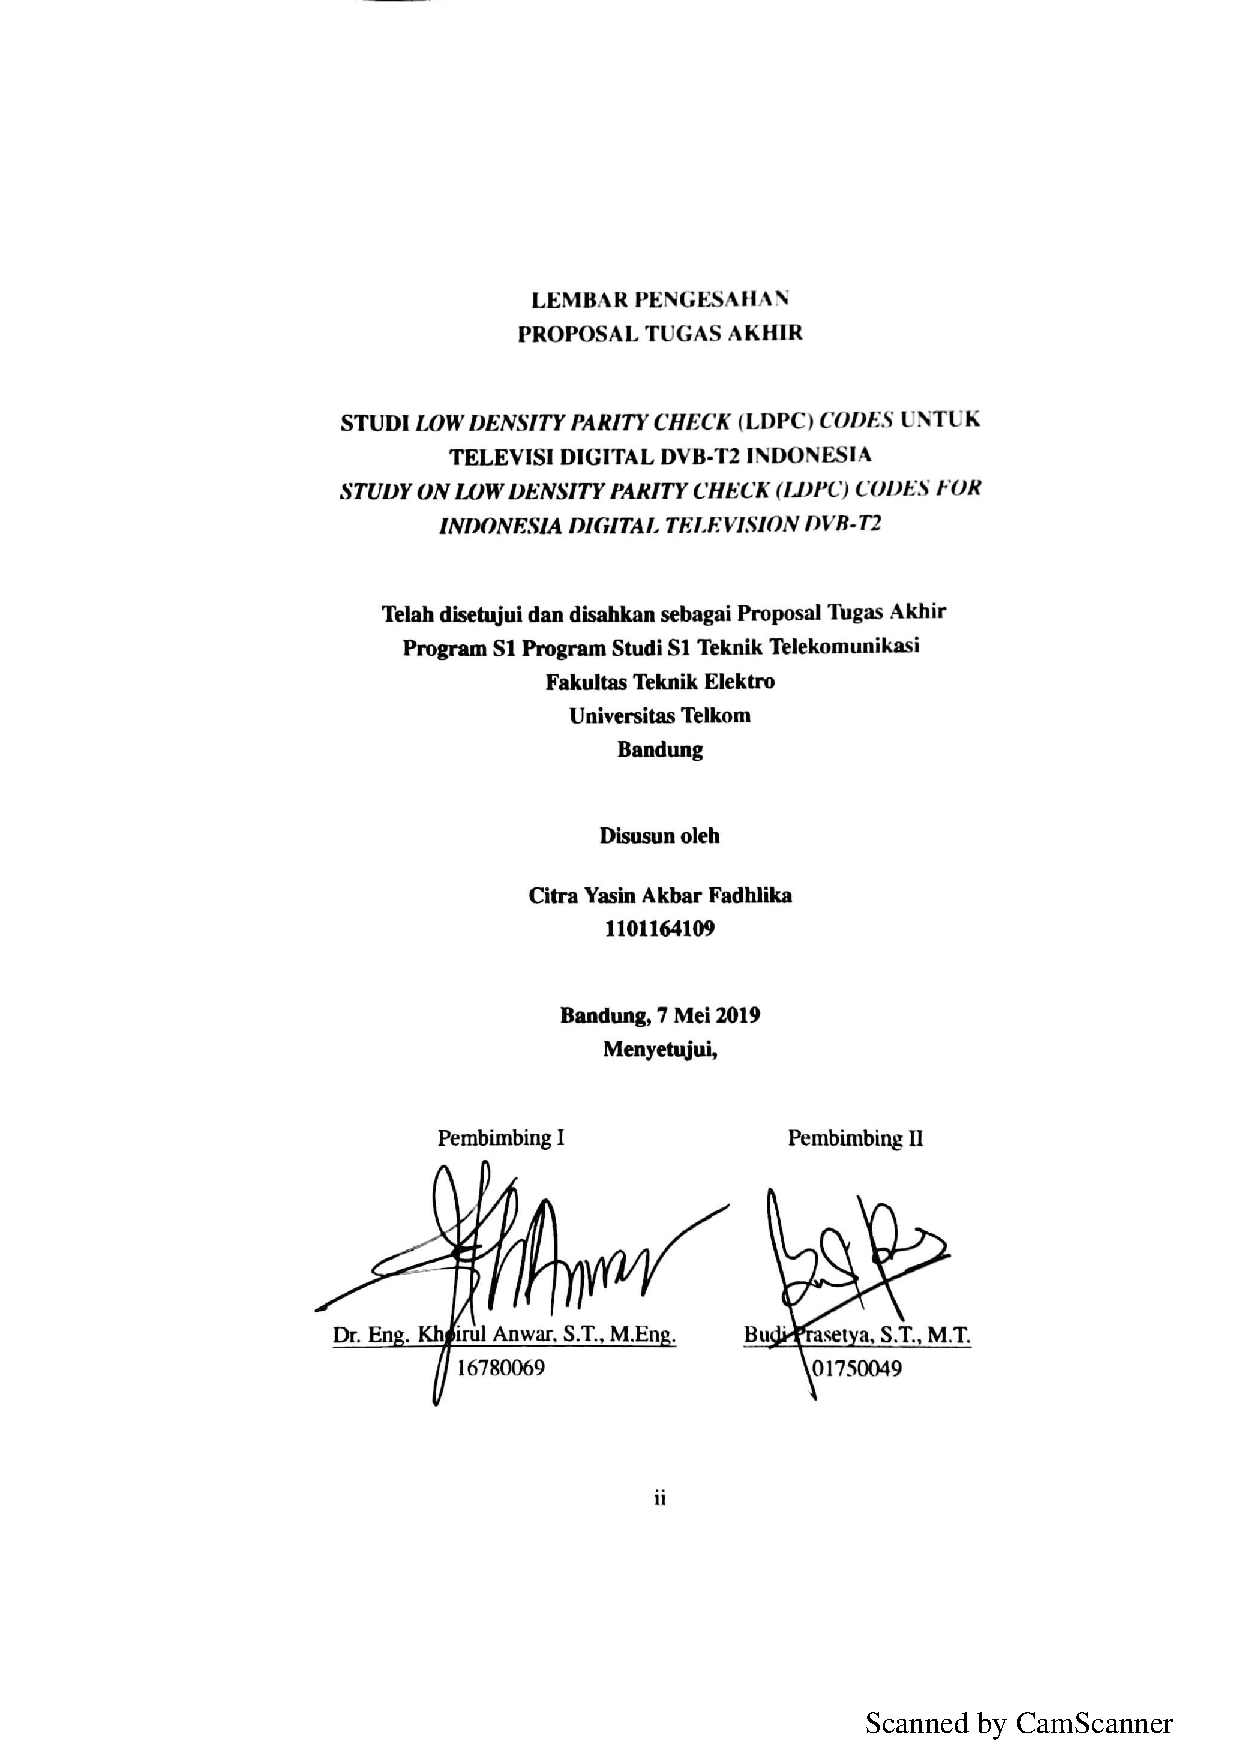
\includepdf[pages=-,pagecommand={},scale=1.18]{pengesah.pdf}
%	
%\end{figure}
%\thispagestyle{empty}
%\include{pengesahan}
\addChapter{LEMBAR PERNYATAAN ORISINALITAS}
\chapter*{}

%\AddToShipoutPicture*{%
%	\gradientbox{white}{white}{%
%		
%		\begin{minipage}[ct][0.98\paperheight][t]{\paperwidth}%
%			\begin{figure}
%				\hspace{1 cm}
%				%        		\vspace{10 cm}
%				%            \begin{center}
%				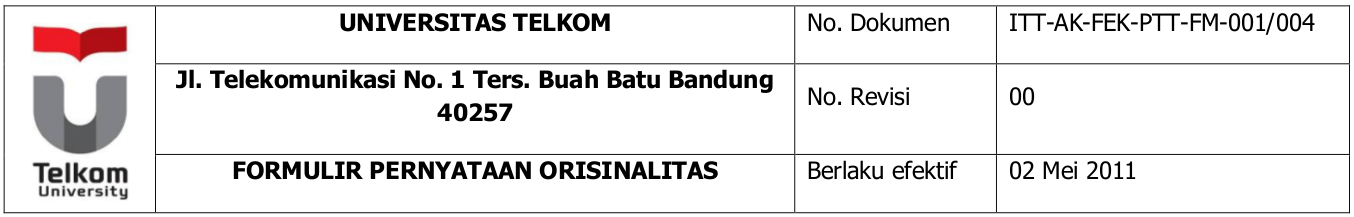
\includegraphics[scale=0.5]{pics/orisinalitas_header.png}
%				%            \end{center}
%			\end{figure}
%\end{minipage}}}

  \begin{center}
 \textbf{LEMBAR PERNYATAAN ORISINALITAS}\\
\end{center}    
\begin{tabular}{ll}
Nama & :\hspace*{0.2 cm}\penulis \\
NIM & :\hspace*{0.2 cm}\nim \\
Alamat & :\hspace*{0.2 cm}\alamat \\
No. Telepon & :\hspace*{0.2 cm}\tlp \\
Email & :\hspace*{0.2 cm}\email \\
\end{tabular}
    
    \vspace*{1 cm}
 Menyatakan bahwa Tugas Akhir ini merupakan karya orisinal saya sendiri, \text{dengan} judul:\begin{center}
\textbf{\Judul}\\
\textit{\textbf{\JudulInggris}}\\
\end{center}
    
    Atas pernyataan ini, saya siap menanggung resiko\slash sanksi yang dijatuhkan kepada saya apabila kemudian ditemukan adanya pelanggaran terhadap kejujuran akademik atau etika keilmuan dalam karya ini, atau ditemukan bukti yang menunjukkan ketidakaslian karya ini.
    
    \vspace*{1 cm}
    
    \begin{tabular}{cl}
    \multirow{6}{*}{
    	\includegraphics[scale=0.035]{pics/IMG0229.jpg}
    	\hspace{5 cm
    }}
    & Bandung, \tanggalPengesahan \\
    & \\
    & \\
    & \penulis \\
    \cline{2-2}
    &  \nim\\
    \end{tabular}

\addChapter{ABSTRAK}

\chapter*{abstrak}
\vspace*{0.7cm}



Tugas Akhir ini melakukan studi pada \textit{Low Density Parity Check} (LDPC) \textit{codes} \textit{Digital Video Broadcasting - Second Generation Terrestrial} DVB-T2 untuk mendapatkan struktur dan kinerja dengan \textit{channel model} Indonesia. Langkah pertama pada Tugas Akhir ini adalah melakukan pengujian \textit{code rate} LDPC \textit{codes} dari standar DVB-T2 pada \textit{channel model} Indonesia. Pengujian dilakukan dengan simulasi komputer menggunakan struktur LDPC \textit{codes} dari standar DVB-T2 sehingga kinerja setiap \textit{code rate} yang berpeluang menjadi standar TV digital Indonesia bisa diketahui. Tugas Akhir ini juga mengusulkan modifikasi LDPC \textit{codes} DVB-T2 untuk menjadi standar LDPC \textit{codes} pada DVB-T2 \text{Indonesia} dengan menggunakan metode \textit{Extrinsic Information Transfer} (EXIT) \textit{analysis}.
%Tugas Akhir ini menguji dan menganalasis perfomansi berbagai \textit{rate} LDPC \textit{Codes} yang telah ditetapkan ETSI sebagai standar DVB-T2.   \textit{Rate} akan dianalisis performansinya dengan parameter \textit{Bit Error Rate} (BER) dan \textit{Block Error Rate} (BLER) yang terbaik. 


	Untuk mengurangi kompleksitas proses komputasi pada \textit{encoder} dan \textit{decoder}, Tugas Akhir ini mengusulkan teknik \textit{downscaling} dengan dan tanpa algoritma \textit{Progresive Edge-Growth} (PEG) untuk LDPC \textit{codes} DVB-T2. Teknik \textit{downscaling} memungkinkan untuk memperpendek panjang LDPC \textit{codes}, sehingga LDPC \textit{codes} DVB-T2 dengan panjang blok 16200 dapat diperkecil menjadi hanya 270. \textit{Downscaled} LDPC \textit{codes} juga diharapkan dapat digunakan untuk perangkat lain dengan daya dan kompleksitas yang rendah.


Tugas Akhir ini menghasilkan beberapa poin berikut ini: (i) struktur LDPC \textit{codes} dengan panjang blok 16200 dan 270 untuk setiap \textit{code rate} yang sesuai \text{dengan} standar DVB-T2, (ii) teknik perancangan LDPC \textit{codes} menggunakan algoritma PEG tanpa adanya \textit{girth} 4 sehingga menjamin \textit{error} yang rendah karena tidak terjadi \textit{cycle} yang melibatkan 4 \textit{nodes}, (iii) teknik untuk menghitung \textit{girth} pada LDPC \textit{codes} yang bermanfaat untuk desain LDPC berbagai ukuran, (iv) kinerja yang baik dari LDPC \textit{codes} DVB-T2 pada kanal \textit{Additive White Gaussian Noise} (AWGN) dan \textit{frequency-selective fading} dengan menggunakan \textit{channel model} DVB-T2 Indonesia. Hasil Tugas Akhir ini diharapkan juga dapat membantu optimalisasi DVB-T2 Indonesia, serta membantu pengembangan LDPC \textit{codes} yang berukuran kecil untuk perangkat berdaya dan kompleksitas rendah, seperti perangkat \textit{Internet of Things} (IoT) dan drone.
%\noindent Abstrak ini\\
%
%{\color{red}nama saya} \\
%\underline{Citra Yasin Akbar Fadhlika}
%\vspace{2cm} %vertikal space
%%\hspace{} untuk horizontal space
%
%Saya tinggal \textit{\textbf{diiiiii}}
%\vspace*{0.2cm}

\noindent Kata Kunci: \textit{\textbf{Error correction coding}}, \textit{\textbf{DVB-T2}}, \textbf{\textit{LDPC} \textit{codes}}, \textbf{\textit{code rate}}


% Abstrak Bahasa Indonesia dan Bahasa Iggris


\chapter*{ABSTRACT}
\vspace*{0.7cm}

This thesis studies Low Density Parity Check (LDPC) codes of Digital Video Broadcasting Second Generation (DVB-T2) to obtain good structure and performances for Indonesia DVB-T2 channel model. The first step of this thesis \text{simulates} performances of LDPC codes from DVB-T2 standard in Indonesia DVB-T2 channel model using computer-based simulation. All the code rates of DVB-T2 LDPC codes are evaluated, of which has a chance to become parameter for digital television standard in Indonesia can be known. This thesis also propose a modified DVB-T2 LDPC codes for standard of Indonesia.

 To reduce the computational complexity of encoder and decoder, this thesis uses a downscaling technique and proposes downscaling technique using Progresive Edge-Growth (PEG) algorithm for LDPC codes of DVB-T2 with a reduced block length of 16200 bits to 270 bits. The results of downscaled LDPC codes are also expected to be used for devices consuming low power and low complexity such as device for Internet of Things (IoT) and drones. 

This thesis obtained following results: (i) the structure of DVB-T2 LDPC codes with block length 16200 and 270 for each code rate, (ii) a technique for designing LDPC codes without girth 4 for LDPC codes construction, (iii) proposed technique to calculate girth from LDPC codes, and (iv) the simulation results showing \text{acceptable} Bit Error Rate (BER) performances of DVB-T2 LDPC codes under \text{Additive} White Gaussian Noise (AWGN) and frequency selective fading channel using Indonesia DVB-T2 channel model. The results of this thesis are expected to fasten the DVB-T2 implementation in Indonesia and assist in the development of small-sized LDPC codes for devices with low power and complexity.

%
% Tugas Akhir ini melakukan studi LDPC \textit{codes} DVB-T2 untuk mendapatkan struktur dan nilai \textit{code rate} yang sesuai dengan \textit{channel model} Indonesia. Langkah pertama adalah melakukan pengujian \textit{code rate} LDPC \textit{codes} dari standar DVB-T2 pada \textit{channel model} Indonesia. Pengujian dilakukan dengan simulasi komputer menggunakan struktur LDPC \textit{codes} dari standar DVB-T2 sehingga \textit{code rate} yang terbaik akan diusulkan untuk menjadi standar TV digital Indonesia. Apabila hasil evaluasi ini menunjukkan bahwa semua \textit{code rate} tidak sesuai dengan \textit{channel model} \text{Indonesia}, maka langkah kedua Tugas Akhir ini mengusulkan modifikasi LDPC \textit{codes} DVB-T2 untuk menjadi standar LDPC \textit{codes} pada DVB-T2 \text{Indonesia} dengan menggunakan metode \textit{Extrinsic Information Transfer} (EXIT) \textit{chart}.
%%Tugas Akhir ini menguji dan menganalasis perfomansi berbagai \textit{rate} LDPC \textit{Codes} yang telah ditetapkan ETSI sebagai standar DVB-T2.   \textit{Rate} akan dianalisis performansinya dengan parameter \textit{Bit Error Rate} (BER) dan \textit{Block Error Rate} (BLER) yang terbaik. 
%
%Hasil yang diharapkan dari Tugas Akhir ini adalah: (i) struktur LDPC \textit{codes} dan nilai \textit{code rate} yang sesuai dengan \textit{channel model} Indonesia sehingga kinerja FEC DVB-T2 optimal dan (ii) kinerja LDPC \textit{codes} DVB-T2 pada \textit{Additive White Gaussian Noise} (AWGN) dan \textit{frequency-selective fading} \textit{channel} menghasilkan nilai \textit{Bit Error Rate} (BER) kurang dari $10^{-3}$. Hasil Tugas Akhir diharapkan juga dapat membantu proses pembuatan standar DVB-T2 Indonesia sehingga dapat mempercepat migrasi DVB-T ke DVB-T2 di Indonesia.
%\noindent Abstrak ini\\
%
%{\color{red}nama saya} \\
%\underline{Citra Yasin Akbar Fadhlika}
%\vspace{2cm} %vertikal space
%%\hspace{} untuk horizontal space
%
%Saya tinggal \textit{\textbf{diiiiii}}
%\vspace*{0.2cm}

\noindent Keywords: \textit{\textbf{Error correction coding}}, \textit{\textbf{DVB-T2}}, \textbf{\textit{LDPC} \textit{codes}}, \textbf{\textit{code rate}}\\ 

\addChapter{UCAPAN TERIMA KASIH}
%-----------------------------------------------------------------------------%
\chapter*{Ucapan Terima Kasih}
%-----------------------------------------------------------------------------%
Penulis ingin berterima kasih sebesar-besarnya kepada semua pihak yang telah membantu pengerjaan baik secara langsung maupun tidak langsung.
\begin{enumerate}
	\item Allah SWT, atas semua kasih sayang, segala petunjuk, dan hidayah dalam setiap proses kehidupan penulis.
	\item Rasulullah SAW, sebagai suri tauladan yang menginspirasi penulis dalam menjalani hidup dan berusaha menjadi lebih baik. 
\item Kedua orang tua penulis yang tercinta, Bapak Era Revianto dan Ibu Ciptani Tresnowati yang tidak henti-hentinya dalam memberikan dukungan, motivasi, dan doa kepada penulis untuk menjadi pribadi yang lebih baik.
\item Adik penulis, Citra Putra Arrafian yang selalu menjadi teman bermain penulis, sehingga penulis tetap dapat menikmati apa yang dihadapi.
\item Keluarga besar dari Papa dan Mama yang selalu memberikan dukungan kepada penulis.
\item Bapak Dr. Eng. Khoirul Anwar, S. T., M. Eng., selaku pembimbing pertama yang selalu memberikan arahan, masukan, dan motivasi kepada penulis dalam menyelesaikan Tugas Akhir ini. Terima kasih telah mengajarkan untuk selalu memberikan yang optimal dalam berkontribusi di dunia ilmu pengetahuan dengan dilandasi kejujuran dan keikhlasan, dan untuk semua nasihat tentang kehidupan yang luar biasa menginspirasi penulis.
\item Bapak Budi Prasetya S.T., M.T., selaku pembimbing kedua yang selalu memberikan masukan dan dukungan untuk saya mengerjakan Tugas Akhir ini dengan sangat baik.
\item Bapak Budi Syihabuddin S.T., M.T., selaku dosen wali yang senantiasa membimbing dan membantu penulis dalam hal akademik selama masa perkuliahan di Telkom University.
\item Bapak Suryo Adhi Wibowo Ph.D., selaku wakil direktur \textit{Center of Advanced for Wireless Technology} (AdWiTech) yang selalu mengingatkan dan memberikan dukungan kepada penulis untuk menyelesaikan Tugas Akhir ini.
\item Seluruh Keluarga Besar AdWiTech yang telah menjadi keluarga penulis selama berkuliah di Telkom University. Terima kasih atas bantuan, ilmu, pengalaman, canda tawa, hiburan, dan bentuk dukungan yang tidak akan penulis lupakan selama masa perjuangan menyelesaikan Tugas Akhir ini.
\item Keluarga besar Laboratorium Dasar Komputer (DasKom), yang telah memberikan kenangan dan motivasi yang luar biasa selama penulis menjalani masa perkuliahan.
\item Seluruh teman-teman Laboratorium \textit{Image Processing and Vision} (IMV) yang selalu berbaik hati.
\item Teman-teman kelas TT-40-04 yang senantiasa menemani penulis hingga memperoleh gelar Sarjana Teknik bersama-sama.
\item Saudara-saudara 'Kos Normies' yang telah memberikan warna dan kebahagian dalam masa perkuliahan di Telkom University.
\item Seluruh dosen dan civitas akademika Telkom University yang tidak dapat penulis sebutkan satu per satu. Terima kasih waktu, wawasan, nasihat, dan pengalaman yang telah diberikan selama penulis menimba ilmu di Telkom University.
\end{enumerate}
\vspace*{0.1cm}
\begin{flushright}
Bandung, 6 Januari 2020\\[0.1cm]
\vspace*{1cm}
\penulis

\end{flushright}

% Kata Pengantar
\addChapter{\kataPengantar}
%-----------------------------------------------------------------------------%
\chapter*{\kataPengantar}
%-----------------------------------------------------------------------------%
Puji syukur kehadirat Allah SWT, atas segala rahmat, petunjuk, dan hidayah-Nya sehingga Penulis mampu menyelesaikan penyusunan Tugas Akhir ini. Tak lupa shalawat serta salam senantiasa tercurah kepada junjungan Nabi Muhammad S.A.W beserta sahabat dan keluarganya. Tugas Akhir ini dibuat untuk memenuhi syarat kelulusan tahap Sarjana program studi Teknik Telekomunikasi, Fakultas Teknik Elektro, Telkom University. Judul dari Tugas Akhir ini adalah "\textbf{\Judul}".


Sebagian hasil Tugas Akhir ini telah dipublikasikan pada \textit{The 3rd International Conference on Symposium on Future Telecommunication Technologies}  (SOFTT) 2019 pada 18-19 November 2019 di Kuala Lumpur, Malaysia.


Penulis menyadari bahwa masih terdapat banyak kekurangan pada Tugas Akhir ini. Oleh karena itu, saran dan kritik yang membangun dari pembaca sangat diharapkan untuk perbaikan. Kritik dan saran dapat disampaikan, semoga Tugas Akhir ini dapat bermanfaat bagi pembaca khususnya dan bagi perkembangan telekomunikasi pada umumnya, terutama di Indonesia.
 
\vspace*{0.1cm}
\begin{flushright}
Bandung, \tanggalPengesahan\\[0.1cm]
\vspace*{1cm}
\penulis

\end{flushright}

% Daftar isi, gambar, dan tabel
\tableofcontents
\clearpage
\listoffigures
\clearpage
\listoftables
\clearpage
% Daftar Lampiran
%\addChapter{DAFTAR LAMPIRAN}
%%-----------------------------------------------------------------------------%
\chapter*{Daftar Lampiran}
%-----------------------------------------------------------------------------%
\noindent
Lampiran A: Data Hasil Pengukuran\\
Lampiran B: Kode Program

\addChapter{DAFTAR \textit{ACHIEVEMENT}}
\chapter*{DAFTAR \textit{ACHIEVEMENT}}

C. Y. A. Fadhlika and K. Anwar, "\textit{Downscaled LDPC Codes for Indonesia Digital Video Broadcasting Terrestrial 2nd Generation} (DVB-T2)”, dipublikasikan pada \textit{International Conference on}
\textit{Symposium of Future Telecommunication Technologies} (SOFTT) 2019, Kuala
Lumpur, Malaysia, November 2019.

% Gunakan penomeran Arab (1, 2, 3, ...) setelah bagian ini.
\pagenumbering{arabic}


% Bab 1 : Pendahuluan
%-----------------------------------------------------------------------------%
 \chapter{\babSatu}
%-----------------------------------------------------------------------------%
%-----------------------------------------------------------------------------%
\section{Latar Belakang Masalah}
%-----------------------------------------------------------------------------%\todo{Ceritakan latar belakang penelitian ini.}
\begin{figure}[b!]
	\centering
	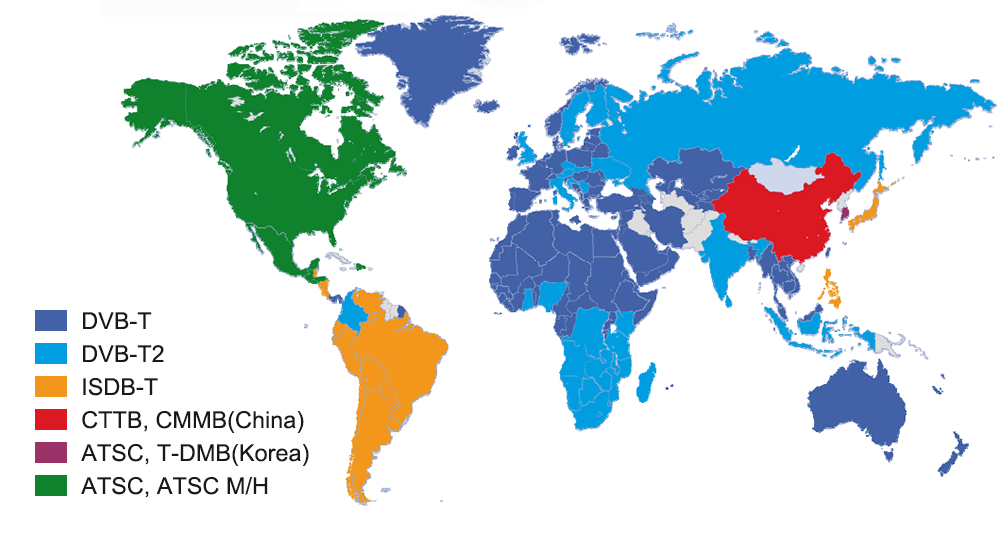
\includegraphics[width=1\textwidth]
		{pics/standar.png}
		\caption{Klasifikasi standar TV digital dunia.}
	\label{fig:Klasifikasi Standar TV Digital Dunia}
\end{figure}
Indonesia telah melakukan migrasi dari penyiaran televisi (TV) analog ke TV digital dengan menggunakan standar \textit{Digital Video Broadcasting-Terrestrial} \text{(DVB-T)} sejak tahun 2007 \cite{regul2}. Saat ini, perkembangan TV \text{digital} di dunia sangat pesat. Berbagai negara telah menggunakan standar \text{\textit{Digital Video Broadcasting - Second Generation Terrestrial}} (DVB-T2) menggantikan standar DVB-T dikarenakan DVB-T2 menggunakan besar spektrum yang sama, tetapi dapat mengirimkan lebih banyak program siaran TV atau dapat mengirimkan kualitas video/audio yang lebih baik daripada DVB-T \cite{itu}. Indonesia diharapkan di masa mendatang dapat melakukan transisi dari DVB-T ke DVB-T2 secara menyeluruh, sesuai dengan regulasi dari Menteri Komunikasi dan Infomatika (Menkominfo) DVB-T2 akan menggantikan standar DVB-T di Indonesia \cite{regul}.

Transisi dari DVB-T ke \text{DVB-T2} memerlukan banyak persiapan. Untuk memperoleh kinerja optimal standar DVB-T2 harus disesuaikan dengan kondisi alam (\textit{channel model}) Indonesia. DVB-T2 menggunakan \textit{Low Density Parity Check} (LDPC) \textit{codes} sebagai \textit{channel coding} di \textit{inner coding} dari \textit{Frame Error Correction} (FEC) \cite{etsi1}. Untuk melakukan migrasi dari DVB-T ke DVB-T2 di Indonesia struktur dan \textit{code rate} LDPC \textit{codes} DVB-T2 yang sesuai dengan \textit{channel model} \text{Indonesia} diperlukan. Penyesuaian LDPC \textit{codes} DVB-T2 diperlukan agar LDPC \textit{codes} dapat bekerja secara optimal, sehingga memiliki peluang \textit{error} menjadi sangat kecil. 

Tantangan utama untuk melakukan transisi dari DVB-T ke DVB-T2 adalah standar DVB-T2 yang diterbitkan oleh \textit{European Telecommunications Standards Institute} (ETSI), merupakan standar untuk menerapkan DVB-T2 di Jerman \cite{etsi2}. Indonesia memiliki \textit{channel model} yang sangat berbeda dari Jerman, oleh karena itu diperlukan standar DVB-T2 yang sesuai dengan \textit{channel model} di Indonesia sehingga DVB-T2 dapat memperoleh kinerja yang optimal. Tugas Akhir ini bertujuan memperoleh standar FEC di bagian \textit{inner coding} dari DVB-T2 yang sesuai dengan \textit{channel model} Indonesia untuk penerapan DVB-T2 di Indonesia kedepannya.   

Hasil yang diharapkan dari Tugas Akhir ini adalah struktur dan \textit{code rate} optimal dari LDPC \textit{codes} DVB-T2 yang sesuai dengan \textit{channel model} \text{Indonesia}. Pengujian kinerja menggunakan metode \textit{Extrinsic Information Transfer} (EXIT) \textit{chart} serta simulasi pada kanal \text{\textit{Additive White Gaussian Noise}} (AWGN) dan \textit{frequency-selective} \textit{fading} menggunakan aplikasi MATLAB, hasil divalidasi \text{dengan} teori dasar, sehingga hasil kinerja \textit{inner coding} dari FEC DVB-T2 ini optimal. 

%-----------------------------------------------------------------------------%
\section{Rumusan Masalah}
%-----------------------------------------------------------------------------%
Sejak tahun 2012 Menkominfo telah menetapkan DVB-T2 sebagai standar penyiaran TV digital di Indonesia \cite{regul}, tapi sampai saat ini Indonesia belum memiliki standar spesifikasi DVB-T2 yang sesuai dengan \textit{channel model} Indonesia. Salah satu spesifikasi DVB-T2 adalah \textit{inner coding} dari FEC DVB-T2 yaitu LDPC \textit{codes}. Tidak adanya struktur optimal ini menyebabkan tidak diketahuinya karakteristik kinerja DVB-T2 Indonesia yang menyebabkan sulitnya industri membuat produk yang terbaik dan sesuai standar Indonesia.

%-----------------------------------------------------------------------------%
\section{Tujuan Penelitian}

Tugas Akhir ini bertujuan melakukan studi pada struktur dan nilai \textit{code rate} LDPC \textit{codes} DVB-T2 yang dievaluasi dengan \textit{channel model} Indonesia, sehingga kinerja TV digital Indonesia bisa diketahui. Hasil ini bermanfaat juga bagi industri dalam mengembangkan alat-alat pemancar dan penerima TV digital.


%-----------------------------------------------------------------------------%
\section{Batasan Masalah}
Tugas Akhir ini memiliki batasan masalah sebagai berikut:
\begin{enumerate}
	\item Menguji kinerja LDPC \textit{codes} DVB-T2 menggunakan \textit{code rate} $\frac{1}{2}, \frac{3}{5}, \frac{2}{3}, \frac{3}{4}, \frac{4}{5},$ dan $\frac{5}{6}$ pada DVB-T2 LDPC \textit{codes} dengan panjang blok $N_{LDPC}=16200$.
	\item Simulasi menggunakan kanal AWGN dan \textit{frequency selective fading} pada \textit{channel model} DVB-T2 di Indonesia.
	\item Untuk simplifikasi penelitian, maka penulis menggunakan modulasi \textit{Quadrature Phase Shift Keying} (QPSK).     	 
\end{enumerate}
%
%Agar penelitian ini dapat memiliki kualitas baik, Tugas Akhir ini membatasi pokok bahasan hanya pada LDPC \textit{codes} yang sesuai dengan standar DVB-T2. Tugas Akhir ini menganalisis kinerja LDPC \textit{codes} menggunakan analisis EXIT \textit{chart}, lalu mensimulasikan kinerja \textit{codes} menggunakan AWGN dan \textit{frequency-selective fading channel}. Apabila tidak ada LDPC \textit{codes} yang optimal dari standar DVB-T2, maka Tugas Akhir ini akan memodifikasi LDPC \textit{codes} dari DVB-T2 agar memiliki kinerja optimal untuk Indonesia.           
%
%Untuk menghindari pembahasan yang terlalu luas, Proposal Tugas Akhir ini hanya akan membahas, diantaranya :
%\begin{itemize}
%	\item[a.]Nilai \textit{rate} dari LDPC \textit{code} yang cocok dengan kanal Indonesia.
%	\item[b.]Merancang LDPC \textit{code} DVB-T2 yang sesuai dengan kanal Indonesia. 
%	\item[c.]Nilai BER, BLER, \textit{outage probability} dari LDPC \textit{code} DVB-T2 yang sesuai dengan kanal Indonesia. 
%\end{itemize}

\section{Metodologi Penelitian}
Tugas Akhir ini menerapkan metodologi penelitian sebagai berikut:	
\begin{itemize}
	\item[a.] Studi Literatur\\	
	Tahap ini melakukan pengumpulan informasi, menganalisis, dan mengidentifikasi tentang LDPC \textit{codes} secara umum dan LDPC \textit{codes} DVB-T2 dari berbagai literatur. Literatur yang menjadi rujukan adalah \textit{text book}, \textit{thesis}, buku disertasi, standar DVB-T2, dan jurnal atau \textit{paper conference} internasional yang dipublikasikan \textit{Institute of Electrical and Electronics Engineers} (IEEE).
	\item[b.] Simulasi pada Kanal AWGN dan \textit{Frequency Selective} \textit{Fading}\\
	Tahap ini bertujuan untuk mengevaluasi kinerja LDPC \textit{codes} DVB-T2 pada kanal AWGN dan \textit{channel model} DVB-T2 Indonesia.
	\item[c.] Perancangan Struktur\\	
	Tahap ini melakukan perancangan struktur LDPC \textit{codes} berdasarkan hasil yang didapat pada tahap (b), jika hasil sudah sesuai, maka perancangan struktur \textit{code} yang baru menjadi minimal. Apabila hasil kurang bagus, maka perancangan struktur akan cukup banyak. 
%	melakukan simulasi menggunakan aplikasi komputer Matlab dari LDPC \textit{codes} DVB-T2 dengan menggunakan \textit{code rate} yang tersedia di standar DVB-T2 pada AWGN dan frekuensi selektif \textit{fading channel}, lalu dioptimalisasi menggunakan EXIT \textit{chart}.
	\item[d.] Analisis EXIT \textit{Chart}\\
	Tahap ini menganalisis struktur dan \textit{code rate} dari LDPC \textit{codes} DVB-T2 untuk menghasilkan kurva EXIT \textit{chart} yang tidak berpotongan  untuk mengetahui kinerja yang paling baik.  
	\item[e.] Studi Analisis\\
	Tahap ini menganalisis hasil simulasi dari semua \textit{code rate} LDPC \textit{codes} DVB-T2 pada tahap sebelumnya. Analisis dilakukan terhadap EXIT \textit{chart}, \textit{girth}, dan kinerja \textit{Bit Error Rate} (BER) pada kanal AWGN dan \textit{frequency-selective fading} menggunakan \textit{channel model} DVB-T2 Indonesia
%	AWGN dan frekuensi selektif \textit{fading channel} yang dibandingkan dengan \textit{shannon-limit} serta dievaluasi menggunakan metode EXIT \textit{chart}. Apabila tidak ditemukan struktur dan \textit{code rate} yang memiliki kinerja optimal dengan parameter gap \textit{shannon-limit} kurang dari 1 dB dan kurva dari EXIT chart tidak saling  berpotongan, 
	\item[f.] Penarikan Kesimpulan\\
	Tahap ini menarik kesimpulan dari seluruh hasil evaluasi dan usulan untuk LDPC \textit{codes} pada DVB-T2.  
\end{itemize}

%\section{Jadwal Pelaksanaan}
%%-----------------------------------------------------------------------------%
%Rencana jadwal penelitan Tugas Akhir ini adalah sebagai berikut: \\
%\begin{table}
%\centering
%\caption{Jadwal penelitian}
%
%	\begin{tabular}{| c | L{4cm} | L{1.8cm} | L{3cm} | L{3.5cm} |}
%		\hline
%		\thead{No.} & \thead{Deskripsi Tahapan} & \thead{Durasi} & \thead{Tanggal Selesai} & \thead{\textit{Milestone}}\\
%		\hline
%		1 & Studi struktur LDPC \textit{codes} & 2 minggu & 20-5-2019 & Perbedaan LDPC \textit{codes} umum dan LDPC \textit{codes} DVB-T2 didapat.\\
%		\hline
%		2 & Simulasi pada AWGN \textit{channel} dan \textit{frequency selective fading channel} & 3 minggu & 10-6-2019 & Gap kurang dari 1~dB dengan \textit{Shannon-Limit}.\\
%		\hline
%		3 & Perancangan struktur & 4 minggu & 8-7-2019 & Struktur LDPC \textit{codes} DVB-T2.\\
%		\hline
%		4 & Analisis EXIT \textit{chart} & 3 minggu & 29-7-2019 & Gap terkecil dan tidak saling berpotongan. \\
%		\hline
%		5 & Analisis & 6 minggu & 9-9-2019 & Menentukan perlunya modifikasi dan melakukan modifikasi.\\
%		\hline
%		6 & Penyusunan buku TA & 2 minggu & 23-9-2019 & Buku TA selesai.\\
%		\hline
%%		5 & Analisis performansi & 3 minggu & 2 Juli 2019 & Menganalisis hasil simulasi yang telah dilakukan\\
%%		\hline
%%		6 & Evaluasi simulasi pertama & 3 minggu & 23 Juli 2019 & Mengevaluasi hasil yang telah dianalisis pada tahapan sebelumnya\\
%%		\hline
%%		7 & Simulasi model kedua & 2 bulan & 23 September 2019 & Perancangan dan simulasi BER, BLER, dan \textit{outage probability} dari hasil evaluasi pertama\\
%%	\hline		
%%		8 & Analisis performansi kedua & 3 minggu & 14 Oktober 2019 & Menganalisis hasil simulasi kedua yang telah dilakukan\\
%%		\hline
%%9 & Evaluasi simulasi & 3 minggu & 4 November 2019 & Mengevaluasi hasil analisis performansi kedua\\
%%	\hline
%%10 & Pengajuan \textit{paper} & 4 minggu & 4 Desember 2019 & Menyusun dan menyelesaikan \textit{paper}\\
%%\hline
%%11 & Penyusunan laporan/buku TA & 3 minggu & 28 Desember 2019 & Buku TA selesai\\
%%\hline
%	\end{tabular}
%	
%\end{table}
\section{Sistematika Penulisan}
%-----------------------------------------------------------------------------%
Untuk selanjutnya, Tugas Akhir ini ditulis dengan sistematika sebagai berikut:
\begin{itemize}
%	\item Bab 1 \babSatu \\
%	Bab ini berisi latar belakang, permasalahan, tujuan, metode penelitian, dan sistematika penulisan dari Tugas Akhir.
	\item BAB II \babDua \\
	Bab ini menjelaskan teori dan dasar LDPC \textit{codes}, DVB-T2, dan pendukung penelitian Tugas Akhir ini.
	\item BAB III \babTiga \\
	Bab ini menjelaskan model sistem mulai dari \textit{transmitter}, model kanal, hingga \textit{receiver}, dan posisi LDPC \textit{codes} dalam sistem tersebut. Bab ini juga menjelaskan LDPC \textit{codes} yang diusulkan.	
	\item BAB IV \babEmpat \\
	Bab ini menganalisis dan mengevaluasi kinerja LDPC \textit{codes} DVB-T2 pada kanal AWGN dan \textit{channel model} DVB-T2 Indonesia yang divalidasi dengan parameter praktis BER.
	\item BAB V \babLima \\
	Bab ini berisi kesimpulan hasil studi kinerja LDPC \textit{codes} DVB-T2 dan saran untuk pengembangan lebih lanjut Tugas Akhir ini pada masa mendatang.
\end{itemize}
%\section{Rumusan}
%Ini lhooo
%\begin{itemize}
%\item [1.] apa kah ini \ref{rumus}?
%\item [2.] ini apa ?
%\end{itemize}
%\subsection{Masalah}
%\cite{buku1}
%\begin{figure}
%\centering
%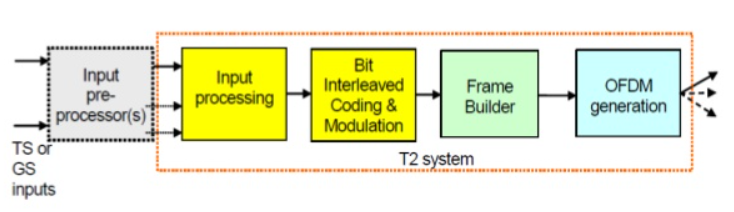
\includegraphics[scale=0.5]{pics/saaa}
%\caption{layer}
%\label {Gambar 1.1: layer}
%\begin{equation}
%\sum_{0}^{100}=\int_{X}^{Y}\cdot\vartheta
%\end{equation}
%\begin{eqnarray}
%\sum_{0}^{100}&=&\int_{X}^{Y}\cdot\vartheta\\
%\sum_{0}^{100}&=&\vartheta
%\label{rumus}
%\end{eqnarray}
%\end{figure}
%\begin{table}
%\begin{center}
%\caption{Perubahan panjang bahan antena}
%\label{tabel: table_tebal}
%\begin{tabular}{|c|c|}
%\hline
%\cellcolor{cyan}Ketebalan bahan & Nilai\\
%\hline
%0.3 cm & -10.64 db\\
%\hline
%\multicolumn{2}{|c|}{0.2cm}\\
%\hline
%0.7 cm & -9.06 db \\
%\hline
%0.1 cm & \multirow{2}{*}{coba}\\
%\cline{1-1}
%0.5 cm & \\
%\hline
%
%
%
%\end{tabular}
%\end{center}
%\end{table}




% Bab 2 : Dasar Teori
%-----------------------------------------------------------------------------%
\chapter{\babDua}
%-----------------------------------------------------------------------------%
%-----------------------------------------------------------------------------%
Bab ini membahas tentang konsep dan teori yang mendasari penelitian Tugas Akhir ini yang meliputi tentang DVB-T2, LDPC \textit{codes}, standar LDPC \textit{codes} DVB-T2, algoritma \textit{Progressive Edge-Growth} (PEG) untuk LDPC \textit{codes}, modulasi QPSK, \textit{Orthogonal Frequency Division Multiplexing} (OFDM), pemodelan kanal yang digunakan, dan EXIT \textit{chart}.


%-----------------------------------------------------------------------------%
\section{\textit{Digital Video Broadcasting – Second Generation Terrestrial} (DVB-T2)}
%-----------------------------------------------------------------------------%
DVB-T2 merupakan standar untuk penyiaran televisi digital yang telah ditetapkan oleh ETSI. DVB-T2 memiliki kinerja lebih baik daripada generasi sebelumnya yaitu DVB-T. DVB-T2 memiliki banyak perbedaan dengan DVB-T salah satunya adalah FEC DVB-T2 yang menggunakan Bose Chaudhuri Hocquenghem (BCH) \textit{codes} dan LDPC \textit{codes}. Dampak penggunaan FEC ini, memberikan keunggulan pada DVB-T2, sehingga memiliki laju data yang lebih cepat $30\%$ daripada DVB-T dan memungkinkan DVB-T2 untuk menggunakan 256-QAM, \textit{Fast Fourier Transform} (FFT) \textit{size} sebesar 16K dan 32K, serta diagram konstelasi yang berotasi. \text{Akibatnya}, memungkinkan untuk mengirimkan kualitas video \textit{High Definition Television Video} (HDTV) \cite{etsi2}.

\begin{table} [tb]
	\renewcommand{\figurename}{Table}
	\centering 
	\caption{Distribusi \textit{column weight} LDPC \textit{codes} DVB-T2 \textit{short frame}.}
	\label{table:dvb-t2lite}
	\begin{tabular}{|c|c|c|c|c|c|c|c|}
		\hline
		\multicolumn{2}{|c|}{Code rate} & \multicolumn{6}{c|}{Column weight}    \\ \hline
		$R_n$  & $R_e$  & 13   & 12   & 8    & 3     & 2    & 1 \\ \hline
		1/2           & 4/9             &      &      & 1800 & 5400  & 8999 & 1 \\ \hline
		3/5           & 3/5             &      & 3240 &      & 6480  & 6479 & 1 \\ \hline
		2/3           & 2/3             & 1080 &      &      & 9720  & 5399 & 1 \\ \hline
		3/4           & 11/15           &      & 360  &      & 11520 & 4319 & 1 \\ \hline
		4/5           & 7/9             &      &      &      & 12600 & 3599 & 1 \\ \hline
		5/6           & 37/45           & 360  &      &      & 12960 & 2879 & 1 \\ \hline
	\end{tabular}
	
	
\end{table}

LDPC \textit{codes} merupakan \textit{inner coding} dari FEC DVB-T2, \textit{code rate} dari LDPC \textit{codes} yang telah ditentukan oleh standar dari ETSI, yaitu : $\frac{1}{2}, \frac{3}{5}, \frac{2}{3}, \frac{3}{4}, \frac{4}{5},$ atau $\frac{5}{6}$ \cite{etsi2}. \textit{Code rate} sebesar $\frac{1}{2}$ memiliki perlindungan proteksi maksimal dan laju data minimal, sedangkan untuk \textit{code rate} sebesar $\frac{5}{6}$ memiliki perlindungan proteksi minimal dan laju data maksimal. Sesuai standar ETSI, LDPC \textit{codes} dari DVB-T2 menggunakan struktur \textit{cyclic} di bagian informasi dan struktur \textit{staircase} di bagian \textit{parity}. Untuk panjang blok di LDPC \textit{codes} dapat menggunakan 16.200 blok (\textit{short frame}) yang akan lebih baik untuk laju data rendah dan 64.800 blok (\textit{long frame}) yang akan lebih baik untuk laju data yang lebih tinggi. Pembentukan matriks \textit{parity check} LDPC \textit{codes} DVB-T2 dibuat berdasarkan dari Tabel \textit{Addresses Parity Bit Accumulator}-nya. Kinerja dari LDPC \textit{codes} akan dipengaruhi oleh \textit{code rate}, lebar spektrum frekuensi, \textit{Guard Interval} (GI), panjang \textit{frame}, dan parameter transmisi lainnya.

\begin{table}[tb]
\centering
\caption{\textit{Addresses of parity bit accumulators} untuk $N_{LDPC}=16200$ dengan \textit{code rate} $R_e=\frac{4}{9}$.}
\label{table:adressldpc}
		\begin{tabular}{|l|l|l|lllll}
			\hline
			\multicolumn{1}{|c|}{20} & \multicolumn{1}{c|}{712}  & \multicolumn{1}{c|}{2386} & \multicolumn{1}{c|}{6354} & \multicolumn{1}{c|}{4061} & \multicolumn{1}{c|}{1062} & \multicolumn{1}{c|}{5045} & \multicolumn{1}{c|}{5158} \\ \hline
			\multicolumn{1}{|c|}{21} & \multicolumn{1}{c|}{2543} & \multicolumn{1}{c|}{5748} & \multicolumn{1}{c|}{4822} & \multicolumn{1}{c|}{2348} & \multicolumn{1}{c|}{3089} & \multicolumn{1}{c|}{6328} & \multicolumn{1}{c|}{5876} \\ \hline
			\multicolumn{1}{|c|}{22} & \multicolumn{1}{c|}{926}  & \multicolumn{1}{c|}{5701} & \multicolumn{1}{c|}{269}  & \multicolumn{1}{c|}{3693} & \multicolumn{1}{c|}{2438} & \multicolumn{1}{c|}{3190} & \multicolumn{1}{c|}{3507} \\ \hline
			\multicolumn{1}{|c|}{23} & \multicolumn{1}{c|}{2802} & \multicolumn{1}{c|}{4520} & \multicolumn{1}{c|}{3577} & \multicolumn{1}{c|}{5324} & \multicolumn{1}{c|}{1091} & \multicolumn{1}{c|}{4667} & \multicolumn{1}{c|}{4449} \\ \hline
			\multicolumn{1}{|c|}{24} & \multicolumn{1}{c|}{5140} & \multicolumn{1}{c|}{2003} & \multicolumn{1}{c|}{1263} & \multicolumn{1}{c|}{4742} & \multicolumn{1}{c|}{6497} & \multicolumn{1}{c|}{1185} & \multicolumn{1}{c|}{6202} \\ \hline
			0                        & 4046                      & 6934                      &                           &                           &                           &                           &                           \\ \cline{1-3}
			1                        & 2855                      & 66                        &                           &                           &                           &                           &                           \\ \cline{1-3}
			2                        & 6694                      & 212                       &                           &                           &                           &                           &                           \\ \cline{1-3}
			3                        & 3439                      & 1158                      &                           &                           &                           &                           &                           \\ \cline{1-3}
			4                        & 3850                      & 4422                      &                           &                           &                           &                           &                           \\ \cline{1-3}
			5                        & 5924                      & 290                       &                           &                           &                           &                           &                           \\ \cline{1-3}
			6                        & 1467                      & 4049                      &                           &                           &                           &                           &                           \\ \cline{1-3}
			7                        & 7820                      & 2242                      &                           &                           &                           &                           &                           \\ \cline{1-3}
			8                        & 4606                      & 3080                      &                           &                           &                           &                           &                           \\ \cline{1-3}
			9                        & 4633                      & 7877                      &                           &                           &                           &                           &                           \\ \cline{1-3}
			10                       & 3884                      & 6868                      &                           &                           &                           &                           &                           \\ \cline{1-3}
			11                       & 8935                      & 4996                      &                           &                           &                           &                           &                           \\ \cline{1-3}
			12                       & 3028                      & 764                       &                           &                           &                           &                           &                           \\ \cline{1-3}
			13                       & 5988                      & 1057                      &                           &                           &                           &                           &                           \\ \cline{1-3}
			14                       & 7411                      & 3450                      &                           &                           &                           &                           &                           \\ \cline{1-3}
		\end{tabular}

	
\end{table}

%-----------------------------------------------------------------------------%
\section{\textit{Low Density Parity Check} (LDPC) \textit{Codes}}
%-----------------------------------------------------------------------------%
LDPC \textit{codes} atau dapat disebut juga \textit{Gallager's codes} diusulkan pada tahun 1962 oleh Robert Gallager \cite{ldpc1}. LDPC \textit{codes} merupakan sebuah \textit{channel coding} untuk melakukan \textit{error correction} yang menggunakan pengkodean dengan menggunakan matriks generator berukuran besar yang jumlah elemen 1 lebih sedikit dibandingkan elemen 0, sehingga disebut \textit{low-density codes} \cite{QC1}. Elemen 1 menunjukkan hubungan antara bit masukan \text{dengan} bit keluaran dari LDPC \textit{codes}. MacKay merupakan salah satu peniliti yang telah menunjukkan bahwa LDPC \textit{codes} memiliki kinerja yang mendekati kapasitas Shannon \cite{ldpc3,ldpc4,ldpc5}. 
%LDPC \textit{codes} mampu meningkatkan reliabilitas dengan menambahkan bit \textit{parity} yang dikirimkan bersamaan dengan bit informasi. Reliabilitas LDPC \textit{codes} semakin lebih baik karena sifat \textit{low-density} pada matriks \textit{parity check}-nya, 

Generator matriks LDPC \textit{codes} ($\mathbf{G}$) berfungsi sebagai pembentuk \textit{codeword} dari bit informasi di sisi pengirim dan matriks \textit{parity check} ($\mathbf{H}$) untuk mengembalikan \textit{codeword} menjadi bit informasi. Keduanya harus memenuhi 
\begin{equation}
\mathbf{G} \mathbf{H}^{T} = 0.
\label{eq:GH}
\end{equation}
Jika Persamaan (\ref{eq:GH}) tidak terpenuhi, LDPC \textit{codes} tidak dapat mendeteksi dan mengoreksi \textit{error} atas \textit{codeword} yang diterima. Bentuk matriks \textit{parity check} dari LDPC \textit{codes} disesuaikan dengan panjang blok (N), dimensi (K), redudansi (M), \textit{degree of variable node} ($d_{v}$), dan \textit{degree of check node} ($d_{c}$) dengan 
\begin{equation}
M = N-K,
\label{eq:Redudansi LDPC code}
\end{equation}
maka matriks \textit{parity check} LDPC \textit{codes} memiliki dimensi $M \times N$. \textit{Variable node} digunakan untuk mendeskripsikan setiap kolom dan \textit{check node} untuk setiap baris dari matriks LDPC \textit{codes}. 
%LDPC \textit{codes} terbagi menjadi dua, yaitu: \textit{regular} yang memiliki nilai $d_{v}$ dan $d_{c}$ sama di setiap baris maupun kolom  dan \textit{irregular} memiliki nilai $d_{v}$ dan $d_{c}$ yang berbeda di baris dan kolom yang memiliki kinerja mengungguli \textit{regular} LDPC \textit{codes} \cite{ldpc7}. 

\begin{figure}
	\centering
	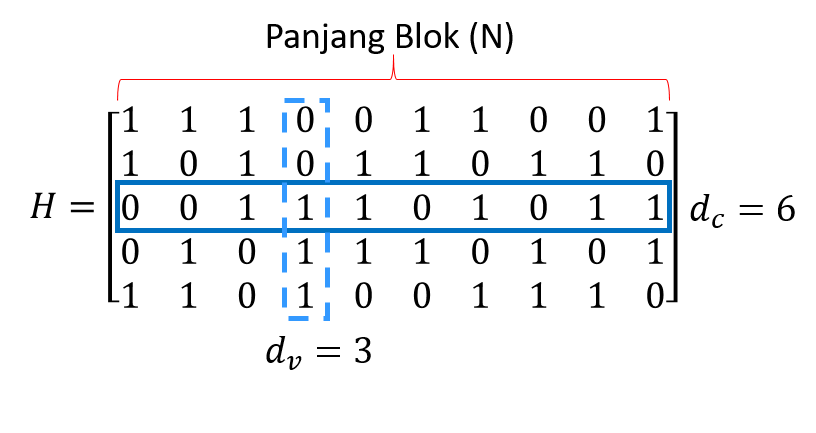
\includegraphics[width=0.6\textwidth]
		{pics/diagram/ldpc.png}
		\caption{Matriks \textit{parity check} \textit{regular} LDPC \textit{codes} (3,6).}
	\label{fig:Regular LDPC codes (3,6)}
\end{figure}
\begin{figure}
	\centering
	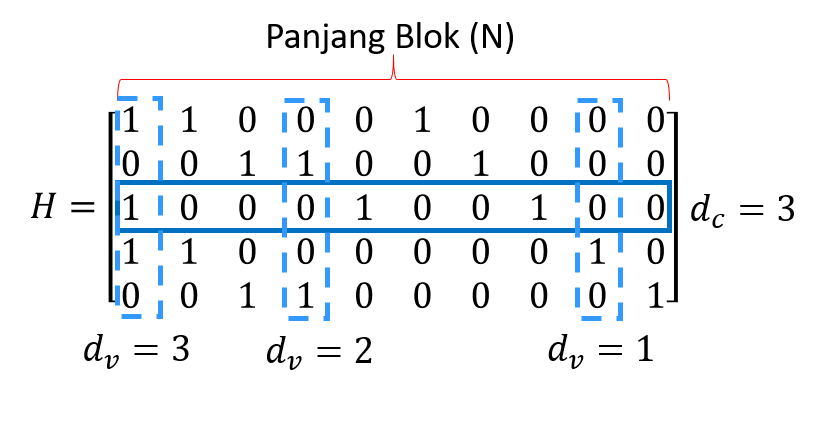
\includegraphics[width=0.6\textwidth]
		{pics/diagram/irre.png}
		\caption{Matriks \textit{parity check} \textit{irregular} LDPC \textit{codes}.}
	\label{fig:Irregular LDPC codes}
\end{figure}
%\textit{Irregular} LDPC \textit{codes} memiliki beban kolom dan beban baris yang berbeda-beda, secara substansial mengungguli \textit{regular} LDPC \textit{codes} \cite{ldpc7}. \textit{Irregular} LDPC \textit{codes} memiliki rumus distribusi kolom $\lambda (x)$ dan distribusi baris $\rho (x)$, sebagai berikut:
%\begin{equation}
%\lambda (x)=\sum_{i= 2}^{dv}\lambda_{i}x^{i-1}
%\label{eq:Distribusi Kolom Kode LDPC Irregular}
%\end{equation}
%\begin{equation}
%\rho (x)=\sum_{i= 2}^{dc}\rho_{i}x^{i-1}
%\label{eq:Distribusi Baris Kode LDPC Irregular}
%\end{equation}
%Dengan asumsi semua persamaan $\lambda (x)$ dan $\rho (x)$ bersifat saling independen secara linier, maka R atau \textit{rate} dari \textit{Irregular} LDPC \textit{codes} adalah 
%\begin{equation}
%R(\lambda,\rho) = 1-\frac{\int_{0}^{1}\rho (x)dx}{\int_{0}^{1}\lambda (x)dx}
%\label{eq:Kode LDPC Irregular}
%\end{equation}
\subsection{Tanner\textit{ Graph}}
Tanner\textit{ graph} merupakan \textit{bipartite graph} yang digunakan untuk menyatakan batasan atau persamaan dari sebuah \textit{error corecting codes} \cite{tann1}. Matriks \textit{parity check} LDPC \textit{codes} dapat direpresentasikan dalam bentuk graf yaitu Tanner\textit{ graph} yang terdiri dari beberapa set \textit{node}. Tanner\textit{ graph} memiliki sebuah garis yang menghubungkan antara \textit{variable node} dan \textit{check node}, jika dan hanya jika \textit{variable node} memiliki hubungan dengan \textit{check node}. Gambar \ref{fig:Tanner Graph LDPC Regular (3,6)} menunjukkan Tanner\textit{ graph} dari matriks \textit{parity check} pada Gambar \ref{fig:Regular LDPC codes (3,6)}, sedangkan Gambar \ref{fig:tg Irregular LDPC codes} merupakan bentuk Tanner\textit{ graph irregular} LDPC \textit{codes} yang memiliki distribusi \textit{variable node degree} (VND) $\Lambda (x)$ dan \textit{check node degree} (CND) $\Omega (x)$ sebagai berikut:
\begin{equation}
 \Lambda (x)=\frac{3}{12}x^{2}+\frac{7}{12}x^{3}+\frac{1}{12}x^{4}+\frac{1}{12}x^{5},
\label{eq:Distribusi var nodes rregular LDPC codes}
\end{equation}
\begin{equation}
 \Omega (x)=\frac{1}{6}x^{4}+\frac{2}{6}x^{5}+\frac{1}{6}x^{6}+\frac{2}{6}x^{7}.
\label{eq:Distribusi check nodes rregular LDPC codes}
\end{equation}
% serta untuk gambar \ref{fig:tg Irregular LDPC codes} Irregular LDPC codes} mewakili \textit{Tanner Graph} dari gambar \ref{fig:Irregular LDPC codes}.
\begin{figure}[tb]
	\centering
	\includegraphics[width=0.35\textwidth]
		{pics/diagram/ldpc2.png}
		\caption{Tanner\textit{ graph} matriks \textit{parity check} \textit{regular} LPDC \textit{codes} dengan $d_{v}=3$ dan $d_{c}=6$.}
	\label{fig:Tanner Graph LDPC Regular (3,6)}
\end{figure} 
\begin{figure}
	\centering
	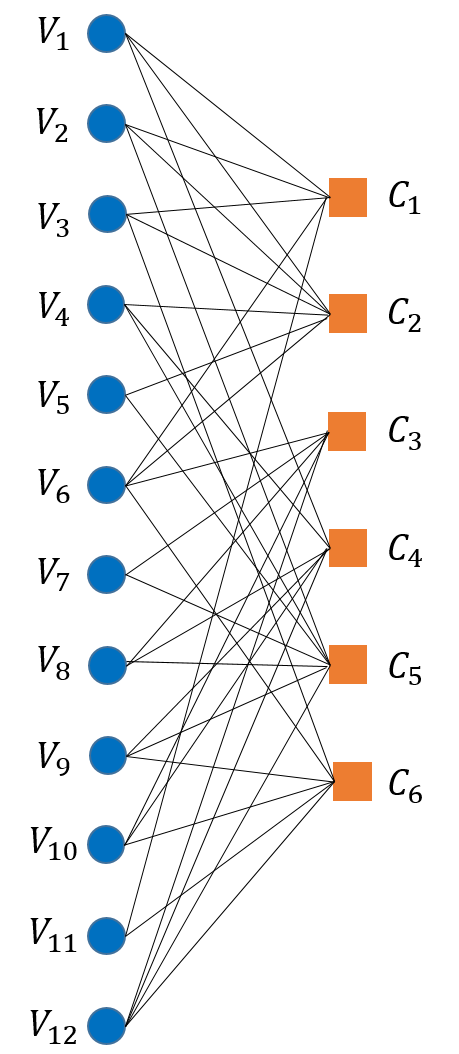
\includegraphics[width=0.32\textwidth]
		{pics/diagram/ldpc3.png}
		\caption{Tanner\textit{ graph} matriks \textit{parity check} \textit{irregular} LDPC \textit{codes} dengan $\Lambda(x)$ pada (\ref{eq:Distribusi var nodes rregular LDPC codes}) dan $\Omega(x)$ pada (\ref{eq:Distribusi check nodes rregular LDPC codes}).}
	\label{fig:tg Irregular LDPC codes}
\end{figure} 

\subsection{\textit{Girth}}
\begin{figure}[b]
	\centering 
	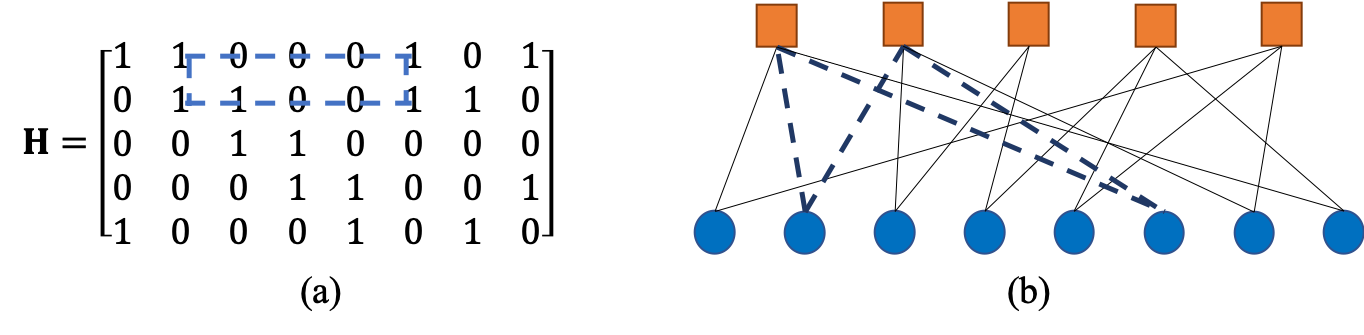
\includegraphics[scale=0.6]{pics/GirthH2}
	\centering 
	\caption{Sebuah contoh \textit{girth} 4 pada LDPC \textit{codes} dengan \textit{cycle} ditunjukkan dengan garis putus-putus: (a) dalam matriks \textit{parity check} $\mathbf{H}$ dan (b) dalam Tanner \textit{graph}.}
	\label{fig:girth}
\end{figure}

	 \textit{Girth} adalah panjang siklus terpendek dalam sebuah Tanner \textit{graph} yang menjadi hal penting dalam menentukan kinerja LDPC \textit{codes} \cite{girth}. Adapun \textit{girth} lokal, \textit{girth} lokal ini terbentuk dari siklus per-\textit{node} pada sebuah Tanner \textit{graph} LDPC \textit{codes}. \textit{Girth} terkecil yang mungkin muncul pada LDPC \textit{codes} adalah \textit{girth} 4, oleh karena itu pada perancangan LDPC \textit{codes} munculnya \textit{girth} 4 harus dihindari. \textit{Girth} dapat dihitung dengan mudah dengan mengamati Tanner \textit{graph} yang terbentuk pada LDPC \textit{codes}. Untuk \textit{girth} 4 dapat diamati melalui matriks \textit{parity check} LDPC \textit{codes} dengan mengamati elemen 1 yang ada, apabila terdapat elemen 1 yang membentuk persegi atau persegi panjang maka \textit{girth} 4 pasti muncul pada LDPC \textit{codes} tersebut seperti pada Gambar \ref{fig:girth}. \textit{Girth} kecil pada LDPC \textit{codes} akan memberikan efek buruk pada LDPC \textit{codes}, karena mengurangi kinerja dari \textit{extrinsic information} dalam proses \textit{iterative decoding} LDPC \textit{codes} \cite{girth2}.

\subsection{\textit{Regular} LDPC \textit{Codes}}
\textit{Regular} LDPC \textit{codes} merupakan struktur LDPC \textit{codes} yang memiliki nilai $d_{v}$ atau banyaknya nilai 1 di setiap kolomnya sama dan nilai $d_{c}$ atau banyaknya nilai 1 di setiap kolomnya sama. Gambar \ref{fig:Regular LDPC codes (3,6)} merupakan contoh matriks dari \textit{regular} LDPC \textit{codes} yang memiliki nilai $N$ sama dengan 10, $d_{v}$ sama dengan 3, dan $d_{c}$ sama dengan 6. Nilai \textit{code rate} \textit{regular} LDPC \textit{codes} dapat diketahui dengan
\begin{equation}
R=1-\frac{d_{v}}{d_{c}}.
\label{code rate regular LDPC codes}
\end{equation}
\subsection{\textit{Irregular} LDPC \textit{Codes}}
\textit{Irregular} LDPC \textit{codes} merupakan jenis struktur dari LDPC \textit{codes} yang memiliki nilai $d_{v}$ dan $d_{c}$ yang tidak sama di setiap baris dan kolomnya, dari segi kinerja \textit{irregular} LDPC \textit{codes} dapat mengungguli \textit{regular} LDPC \textit{codes} \cite{ldpc7}. Hal ini dikarenakan, nilai \textit{girth} dari \textit{irregular} LDPC \textit{codes} cenderung lebih besar dari \textit{regular} LDPC \textit{codes}. \textit{Irregular} LDPC \textit{codes} memiliki persamaan untuk distribusi VND $\Lambda (x)$ dan distribusi CND $\Omega (x)$, sebagai berikut:
\begin{equation}
\Lambda (x)=\sum_{i= 1}^{dv}\Lambda_{i}x^{i},
\label{eq:Distribusi Kolom Irregular LDPC codes}
\end{equation}
\begin{equation}
\Omega (x)=\sum_{i= 1}^{dc}\Omega_{i}x^{i}
\label{eq:Distribusi Baris Irregular LDPC codes}
\end{equation}
dengan asumsi semua persamaan $\Lambda (x)$ dan $\Omega (x)$ bersifat saling independen linier, maka \textit{code rate} $(R)$ dari \textit{irregular} LDPC \textit{codes} adalah 
\begin{equation}
R(\Lambda,\Omega) = 1-\frac{\int_{0}^{1}\Omega (x)dx}{\int_{0}^{1}\Lambda (x)dx}.
\label{eq:Rate Irregular LDPC codes}
\end{equation}

%\subsection{\textit{Quasi-Cyclic} (QC) LDPC \textit{Codes}}
%QC-LDPC \textit{codes} adalah \textit{channel coding} yang memiliki kompleksitas rendah dengan menggunakan struktur dari LDPC \textit{codes} \cite{QC2}. QC-LDPC \textit{codes} memiliki struktur yang terbentuk dari pergeseran sirkular sehingga satu \textit{codeword} yang akan menghasilkan \textit{codeword} lain. Struktur tersebut membuat QC-LDPC \textit{codes} memerlukan memori yang lebih sedikit dibandingkan dengan LDPC \textit{codes} konvensional dan ini merupakan salah satu kelebihan QC-LDPC \textit{codes} \cite{QC3}. Susunan matriks generator dari QC-LDPC \textit{codes} berbeda dengan LDPC \textit{codes} karena QC-LDPC \textit{codes} memiliki matriks yang sirkular. QC-LDPC \textit{codes} memiliki $H_{Q}$ yang terdiri dari beberapa matriks \textit{binary polinomial} yaitu
%\begin{equation}
%H_{Q}(\lambda_{I,J})= \begin{bmatrix} \lambda_{0,0}(U) & \lambda_{0,1}(U) & \cdots & \lambda_{0,J-1}(U) \\ \lambda_{1,0}(U) & \lambda_{1,1}(U) & \cdots & \lambda_{1,J-1}(U) \\ \vdots & \vdots & \ddots & \vdots \\ \lambda_{I-1,0}(U) & \lambda_{I-1,1}(U) & \cdots & \lambda_{I-1,J-1}(U)
%
%\end{bmatrix},
%\label{eq: Matriks Binary Polynomial QC-LDPC}
%\end{equation} 
%
%dengan nilai $I=\{ 0,1,2,\dots,I-1 \}$ adalah jumlah elemen baris dan $J=\{ 0,1,2,\dots,J-1 \}$ adalah elemen kolom matriks $H_{Q}$. Setiap matriks \textit{binary polinomial} $\lambda_{I,J}(U)$ terdiri atas $ZxZ$ matriks \textit{polinomial circular} yaitu
%\begin{equation}
%\lambda_{I,J}(U)= \begin{bmatrix} 
%a_{1} & a_{2} & \cdots & a_{z-1} & a_{z}  \\ 
%a_{z} & a_{1} & \cdots & a_{z-2} & a_{z-1} \\ 
%\vdots & \vdots & \ddots & \vdots & \vdots \\ 
%a_{2} & a_{3} & \cdots & a_{z} & a_{1}
%
%\end{bmatrix}.
%\label{eq: Matriks Binary Polynomial QC-LDPC}
%\end{equation} 
 
\subsection{LDPC \textit{Staircase} \textit{Codes}}
LDPC \textit{Staircase codes} merupakan LDPC \textit{codes} yang menggunakan struktur matriks \textit{lower triangular}. Matriks LDPC \textit{Staircase codes} memiliki bentuk seperti "tangga" yang terbentuk oleh elemen 1, sehingga setiap simbol yang \textit{error} dapat dikoreksi dari nilai jumlah simbol sebelumnya di baris terkait \cite{staircase1}. Matriks \textit{parity check} LDPC \textit{Staircase codes} memiliki bentuk
\begin{equation}
\mathbf{H} = \begin{bmatrix} 
0 & 1 & 1 & 0 & 1 & 0 & \textbf{1} & 0 & 0 & 0  \\ 
1 & 0 & 0 & 1 & 1 & 0 & \textbf{1} & \textbf{1} & 0 & 0  \\ 
0 & 1 & 0 & 1 & 0 & 1 & 0 & \textbf{1} & \textbf{1} & 0  \\ 
1 & 0 & 1 & 0 & 0 & 1 & 1 & 0 & \textbf{1} & \textbf{1} 
\end{bmatrix}.
\label{eq: Matriks Parity Check LDPC-Staircase codes}
\end{equation} 
\noindent Matriks (\ref{eq: Matriks Parity Check LDPC-Staircase codes}) dibagi menjadi dua bagian ($\mathbf{H}_1 \mid \mathbf{H}_2$). $\mathbf{H}_1$ merupakan bagian sebelah kiri matriks $\mathbf{H}$ dari kolom $0$ ke $K-1$ yang mendefinisikan penempatan simbol dari sumber informasi dalam sebuah persamaan linier. $\mathbf{H}_2$ merupakan bagian sebelah kanan matriks $\mathbf{H}$ dari $K$ ke $N-1$ yang mendefinisikan persamaan-persamaan simbol perbaikan pada baris yang berkaitan dan membentuk seperti "tangga". Operasi dasar dalam pembentukan matriks \textit{parity check} LDPC \textit{Staircase codes} menggunakan operasi \textit{exclusive or} (XOR). LDPC \textit{Staircase codes} yang memiliki nilai \textit{code rate} ($R$) setiap $m$ baris dari matriks $\mathbf{H}_1$ akan memiliki \textit{degree}
\begin{equation}
d_{R_{\mathbf{H}_1}}= \frac{N_{1}}{\frac{1}{R}-1}
\label{eq: degree matriks H1}
\end{equation} 
\noindent dengan $N_{1}$ merupakan jumlah banyaknya nilai elemen 1 di setiap kolom matriks $\mathbf{H}_1$ Matriks (\ref{eq: Matriks Parity Check LDPC-Staircase codes}). Akibat dari struktur \textit{staircase} di matriks $\mathbf{H}_2$, satu baris $m$ dari matriks $\mathbf{H}$ akan memiliki \textit{degree}
\begin{equation}
d_{r}(m)=
\left\{\begin{matrix}
d_{r_{\mathbf{H}_1}}+1 \;\;\; if \; m=1,
\\ 
d_{r_{\mathbf{H}_1}}+2 \;\;\; if \; m>1 .
\end{matrix}\right.
\label{eq: degree matriks $H_{1}$}
\end{equation} 
Representasi LDPC \textit{Staircase} \textit{codes} dalam bentuk Tanner\textit{ graph} ditunjukkan oleh Gambar \ref{fig:Tanner Graph LDPC Staircase codes}.

\begin{figure}[t!]
	\centering
	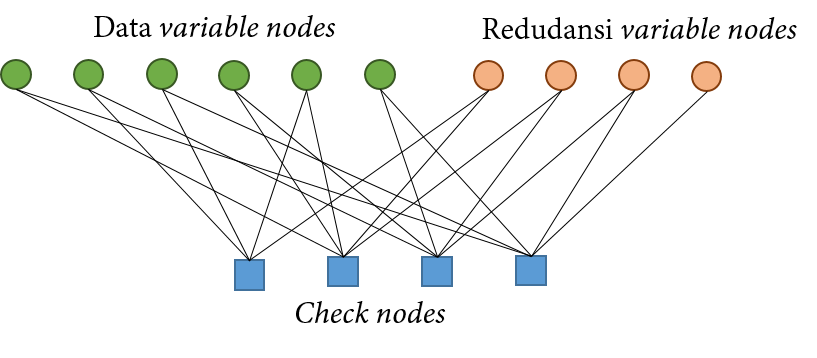
\includegraphics[scale=0.9]
	{pics/staircase.png}
	\caption{\textit{Sebuah Tanner graph} dari LDPC \textit{Staircase codes} dengan $N=10$, $K=6$, dan $N_{1}=2$.}
	\label{fig:Tanner Graph LDPC Staircase codes}
\end{figure}

%\cite{•}
%\cite{•}

%\section{Metode \textit{Downscaled} untuk LDPC \textit{Codes} DVB-T2}
%
%Metode \textit{Downscaled} digunakan untuk mengurangi kompleksitas komputasi dari \textit{encoder} dan \textit{decoder}, sehingga akan meringankan proses simulasi dan memungkinkan untuk \textit{device} dengan kemampuan komputasi rendah \cite{scale}. Langkah-langkah untuk \textit{downscaling} LDPC \textit{codes} DVB-T2 sesuai \cite{scale}, sebagai berikut: 
%
%\begin{enumerate}
%	\item Tentukan \textit{scaling factor} $s_f$, $s_f$ harus merupakan faktor dari $360$. 
%	\item Masukkan nilai pada tabel \textit{addresses of parity bit accumulators} seperti pada Tabel \ref{table:adressldpc} ke $p_{1}(j), p_{2}(j), p_{3}(j), \dots$$, p_{q}(j)$, $j= 1, 2, 3, \dots, J$  dan $q= 1, 2, 3, \dots, Q$. $j$ menunjukkan kolom dan  $q$ menunjukkan baris dari Tabel \ref{table:dvb-t2lite}.
%	\item Hitung $r_{1}(j), r_{2}(j), r_{3}(j), \dots, r_{q}(j)$
%		\begin{equation}
%	r_{q}(j)=mod\left \{ \left [ p_q(j) + J \times \left ( k-1 \right ) \right ],\left [ P/s_f \right ] \right \},
%	\end{equation}
%	\item Nilai $r_q(j)$ akan menjadi tabel \textit{addresses parity bit accumulators} baru untuk \textit{downscaled} LDPC \textit{codes} DVB-T2. 
%\end{enumerate}
%Dengan $q$ adalah kolom dan $j$ baris dari tabel \textit{addresses parity bit accumulators}.  Nilai $s_f$ yang akan membentuk matriks \textit{downscaled} \textit{parity check} LDPC \textit{codes}. $P$ adalah nilai dari $N-K$ matriks LDPC codes original, nilai $k$ memiliki batas dengan $1< k \leq \left ( 360/s_f \right )$. Nilai $360$ adalah jumlah \textit{node indices} LDPC \textit{codes} DVB-T2.
\section{\textit{Accumulator} }
\textit{Accumulator} adalah sebuah teknik yang diadaptasi dari Turbo \textit{codes}, \textit{accumulator} terbukti memiliki kinerja yang baik dalam proses \textit{decoding} dan simpel dalam  pembentukkan generator matriks pada LDPC \textit{codes} \cite{IRA}. Kombinasi antara \textit{accumulator} dengan \textit{irregular} LDPC \textit{codes} terbukti memiliki kinerja yang lebih baik daripada \textit{irregular} LDPC \textit{codes} terbaik yang pernah ada. \textit{Accumulator} memiliki matriks seperti
\begin{equation}
\mathbf{H}= \begin{bmatrix} 
 \textbf{1} & 0 & 0 & 0  \\ 
 \textbf{1} & \textbf{1} & 0 & 0  \\ 
0 & \textbf{1} & \textbf{1} & 0  \\ 
 0 & 0 & \textbf{1} & \textbf{1} 
\end{bmatrix}.
\label{eq: IRA}
\end{equation} 
Gambar \ref{fig:ira codes} menunjukkan struktur dari \textit{accumulator} pada persamaan (\ref{eq: IRA}) memiliki pola \textit{zigzag} dengan proses \textit{decoding} menggunakan operasi XOR.
\section{\textit{Low Density Generator Matrix} (LDGM)}
\begin{figure}[b!]
	\centering
	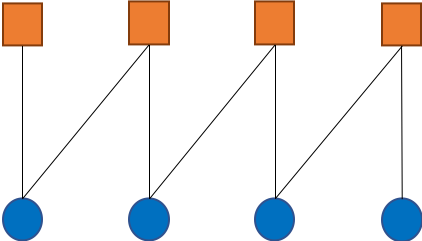
\includegraphics[scale=0.75]
	{pics/ira.png}
	\caption{Sebuah Tanner \textit{graph} untuk \textit{accumulator} dengan $\mathbf{H}$ pada (\ref{eq: IRA}).}
	\label{fig:ira codes}
\end{figure}
Dalam proses pengkodean, \textit{Low Density Generator Matrix} (LDGM) menggunakan operasi XOR. LDGM dapat di-\textit{decode} dengan \textit{Sum Product Algorithm} (SPA). Keuntungan dari pengkodean LDGM adalah proses yang sederhana \cite{LDGM}, karena hanya terdiri dari perkalian matriks dari input simbol dengan matriks \textit{sparse} generator $\mathbf{G}$. Matriks \textit{parity check} $\mathbf{H}$ LDGM \textit{codes} memiliki \textit{degree} satu dengan matriks identitas di dalamnya yang menunjukkan bahwa matriks tersebut sederhana dalam proses pembuatan matriks generator seperti matriks berikut
\begin{eqnarray}
\mathbf{H}=\begin{bmatrix}
0 & 1 & 0 & 0 & 1 & 0 & 0\\
1 & 0 & 1 & 0 & 0 & 1 & 0\\
1 & 0 & 0 & 1 & 0 & 0 & 1
\end{bmatrix}, \;
\mathbf{G}=\begin{bmatrix}
1 & 0 & 0 & 0 & 0 & 1 & 1\\
0 & 1 & 0 & 0 & 1 & 0 & 0\\
0 & 0 & 1 & 0 & 0 & 1 & 0\\
0 & 0 & 0 & 1 & 0 & 0 & 1
\end{bmatrix}.
\end{eqnarray}
LDGM \textit{codes} dikombinasikan dengan LDPC \textit{codes} sebagai \textit{parity} yang berfungsi untuk menjadi \textit{redundancy} dengan memberikan tambahan bit \textit{parity} pada \textit{codeword} $\mathbf{c}$. Parameter $\mathbf{c}$ merupakan bit informasi $\mathbf{b}$ yang telah diberi bit \textit{parity} untuk menambah kemampuan dalam koreksi kesalahan. 

\section{Algoritma \textit{Progressive Edge-Growth} (PEG)}

\textit{Progressive Edge-Growth} (PEG) adalah salah satu metode dalam merancang matriks \textit{parity check} LDPC \textit{codes} berdasarkan dari Tanner \textit{graph} dengan memperhatikan penyebaran \textit{edge} yang terhubung pada setiap \textit{node} untuk menghasilkan \textit{girth} besar \cite{PEG}. Perancangan LDPC \textit{codes} dengan menggunakan PEG dapat dibuat berdasarkan jumlah \textit{variable nodes} atau \textit{block length} $n$, check node $m$, VND, dan CND. PEG melakukan penyebaran \textit{edge} menggunakan graf pohon dengan memperhatikan \textit{degree} setiap \textit{node} yang telah ditentukan dan setiap \textit{node} hanya muncul sekali saja. Kedalaman dari graf pohon akan disimbolkan dengan $l$.

Secara sederhana proses pembuatan LDPC \textit{codes} menggunakan algoritma PEG adalah sebagai  berikut \cite{PEG}:
\begin{enumerate}
	\item Tempatkan elemen 1 mulai dari kolom ke-1 sampai ke-$n$, penempatan ini memperhatikan baris atau \textit{check node} dengan \textit{degree} terkecil.
	\item Menyebarkan \textit{edge} ke \textit{node} yang belum terhubung dengan memperhatikan \textit{degree} dari \textit{check node}.
\end{enumerate}
\textit{Cycle} dari LDPC \textit{codes} yang terbentuk menggunakan PEG dapat dipastikan akan bernilai $2(l+2)$.
%\begin{equation}
%2(l+2).
%\end{equation}
Dalam perancangan LDPC \textit{codes} menggunakan algoritma PEG dengan nilai $d_v$, $d_c$, dan $m$ yang telah ditentukan, dapat diketahui batas dari nilai \textit{girth} melalui persamaan
\begin{equation}
t=\frac{\log\left ( md_c^{max}- \frac{md_c^{max}}{d_v^{max}} - m +1 \right )}{\log\left [ \left ( d_v^{max} -1  \right ) \left ( d_c^{max} -1  \right ) \right ]}-1
\label{eq:t}
\end{equation}
\begin{equation}
g \geq 2 \left (\left \lfloor t \right \rfloor +2 \right ),
\label{eq:g}
\end{equation}
dengan $g$ adalah \textit{girth}, dari Persamaan (\ref{eq:t}) dan (\ref{eq:g}) maka
\begin{equation}
\frac{d_v^{max}\left [  \left ( d_v^{max}-1 \right )^{t+1} \left ( d_c^{max}-1 \right )^{t+1} -1\right ]}{\left ( d_v^{max}-1 \right ) \left ( d_c^{max}-1 \right )-1}<m.
\end{equation}

PEG memiliki dua metode dalam proses perancangan LDPC \textit{codes} dengan cara \cite{PEG2}:
\begin{enumerate}
	\item Secara acak memilih \textit{check nodes} terkecil yang ditemukan.
	\item Selalu memilih \textit{check nodes} terkecil yang ditemukan sesuai dengan urutannya $c_1, c_2, c_3, \cdots, c_{m},$ $m$ adalah jumlah baris.
\end{enumerate}
Hal ini mengakibatkan LDPC \textit{codes} akan memiliki matriks \textit{parity check} berbeda, apabila menggunakan algoritma PEG.


\section{Modulasi}
Modulasi merupakan proses perubahan sebuah gelombang periodik menjadi sebuah sinyal yang mampu membawa informasi. Sinyal informasi akan ditumpangkan pada gelombang radio yang bertugas sebagai sinyal pembawanya (\textit{carrier}). Langkah terbaik untuk mengirimkan informasi yang berupa $+1$ atau $-1$ menggunakan gelombang radio dengan memodulasi sinyal \textit{carrier} dengan frekuensi $f_c$ yang sesuai sinyal informasinya \cite{modul}. Bentuk gelombang dari sinyal \textit{carrier} $S(t)$ dapat dinyatakan sebagai 
\begin{equation}
	S(t) =A \; cos \left \{ 2\pi f_c t + \theta \left( t \right ) \right \}
\end{equation}
dengan A adalah amplitudo, $f_c$ adalah frekuensi tengah, dan $\theta (t)$ adalah fasa sesuai dengan variansi waktu dari gelombang sinyal \textit{carrier}. 



\section{Pemodelan Kanal}
%-----------------------------------------------------------------------------%
Tugas Akhir ini menggunakan pemodelan kanal radio. Terdapat dua paramater utama dalam pemodelan kanal yang dirancang, yaitu adanya \textit{noise} dan terjadinya \textit{multipath fading}. Sub bab ini akan menjelaskan kanal AWGN dan \textit{frequency selective fading}.
%, \textit{Power Delay Profile} (PDP), dan pemodelan kanal Indonesia. 
\subsection{Kanal \textit{Additive White Gaussian Noise} (AWGN)}
\begin{figure}[tp]
	\centering
	
\includegraphics[scale=0.55]
		{pics/awgn1.png}
		\caption{Diagram blok kanal AWGN.}
	\label{fig:Model Channel Model AWGN}
\end{figure}
Kanal AWGN adalah kanal paling populer karena dianggap sebagai model yang baik untuk banyak aplikasi. Kanal AWGN memiliki beberapa karakteristik, antara lain \cite{awgn1}: 
\begin{enumerate}
\item \textit{Additive}, karena \textit{noise} ditambahkan ke simbol-simbolnya.
\item \textit{White}, memiliki rapat daya yang konstan di setiap frekuensi.
\item \textit{Gaussian}, karena \textit{noise} dari kanal AWGN terdistribusi \textit{Gaussian}.
\end{enumerate}
Pemodelan matematika untuk sinyal yang diterima di \textit{receiver} pada kanal AWGN berdasarkan Gambar \ref{fig:Model Channel Model AWGN} adalah 
\begin{equation}
r(t)=s(t)+n(t)
\label{eq:Model Matematika Channel Model AWGN}
\end{equation}
dengan $s(t)$ adalah sinyal yang ditransmisikan, $n(t)$ adalah \textit{white Gaussian noise}, dan $r(t)$ adalah sinyal yang diterima.

Proses transmisi pada kanal AWGN akan disimulasikan dengan menggunakan aplikasi MATLAB. Densitas spektral daya kanal AWGN sama rata untuk semua frekuensi. 
%Sumber \textit{noise} pada kanal AWGN berupa \textit{noise thermal} yang diakibatkan oleh kondisi panas komponen elektronik di \textit{receiver}.
Sinyal yang \text{diterima} dalam aplikasi MATLAB didefinisikan sebagai 
\begin{equation}
\mathbf{r}_{x}=\mathbf{H}\cdot \mathbf{t}_{x}+\mathbf{n}
\label{eq:AWGN matlab}
\end{equation}
dengan $\mathbf{r}_{x}$ merupakan sinyal yang diterima oleh \textit{receiver}, $\mathbf{h}=1$ untuk AWGN \textit{channel}. Parameter $\mathbf{t}_{x}$ adalah sinyal yang dikirimkan dari \textit{transmitter}, dan \textit{noise} $\mathbf{n}$ didefinisikan dengan perintah MATLAB
\begin{equation}
\mathbf{n}=\sigma \cdot (randn(1,B)) + \sqrt{-1} \times (randn(1,B)),
\end{equation}
yang memiliki distribusi Gaussian sepanjang simbol ($B$) dengan varians $\sigma^2$ pada (\textit{double-sided noise}) dan rata-rata nol. Probabilitas fungsi densitasnya adalah
\begin{equation}
p(m)=\frac{1}{\sigma \sqrt{2\pi}}\cdot \exp \left ( -\frac{m^2}{2\sigma ^{2}} \right )
\label{eq:prob dens}
\end{equation}
dengan $m$ adalah \textit{random} variabel dari \textit{noise}.
%$n(t)$ adalah contoh fungsi proses AWGN yang menggunakan proses \textit{probability density function} (pdf) dan rapat daya spektral 
%\begin{equation}
%\Phi_{nn}(f)=\frac{1}{2}N_{0}[W/Hz],
%\label{eq:Noise Channel Model AWGN}
%\end{equation}
%\noindent dengan $N_{0}$ bersifat konstan. AWGN \textit{Channel} memiliki model seperti pada Gambar \ref{fig:Model Channel Model AWGN}.  
\subsection{\textit{Frequency Selective Fading Channel}}
\begin{figure}[tb]
	\centering
	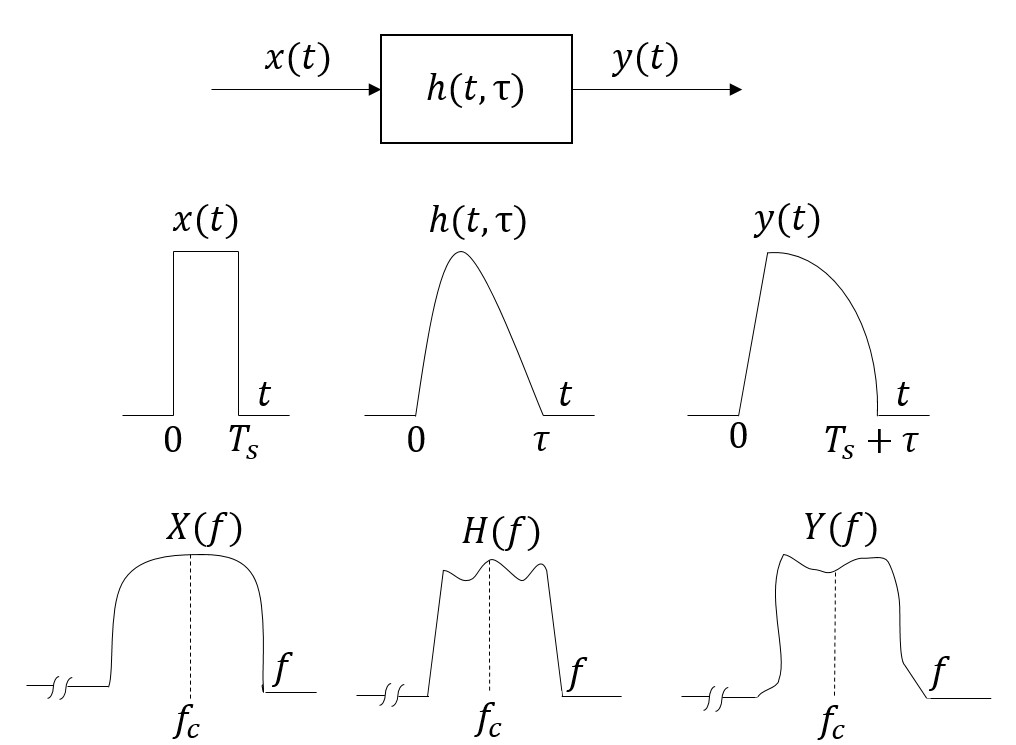
\includegraphics[scale=0.7]
	{pics/fadi.jpg}
	\caption{Karakteristik kanal untuk \textit{frequency selective fading}.}
	\label{fig:Frequency Selective Fading Channel}
\end{figure}
\textit{Frequency selective fading channel} terjadi ketika amplitudo konstan dan respon fasa linier pada \textit{wireless channel} lebih sempit daripada \textit{bandwidth} sinyal, sehingga amplitudo respon frekuensi dari sinyal yang ditransmisikan menjadi bervariasi terhadap frekuensi \cite{fading1}. Gambar \ref{fig:Frequency Selective Fading Channel} menunjukkan karakteristik dari \textit{frequency selective fading channel} dan ilustrasi di \textit{domain} waktu dan frekuensi. 
\textit{Frequency selective fading channel} adalah sebuah \textit{wideband channel} dengan kondisi kanal ($\tau$) lebih besar dari pada periode simbol sinyal yang ditransmisikan ($T_{s}$) atau jika \textit{maximum excess delay} ($T_{m}$) lebih besar daripada ($T_{s}$) \cite{fading2}. Sehingga dapat disimpulkan sinyal dipengaruhi oleh \textit{frequency selective fading channel} jika:
\begin{eqnarray}
B_{s} \geq B_{c},  \nonumber \\ 
 T_{s} \leq \sigma_{\tau}, \nonumber \\ 
T_{s} \leq T_{m}. 
\label{eq:Kondisi Frequency Selective Fading Channel}
\end{eqnarray}
\noindent Oleh karena itu, sebuah kanal dianggap \textit{frequency selective fading channel} ketika $\sigma_{\tau} = 0.1 T_{s}$.

%\section{Kanal \textit{Broadband}}
%Kanal \textit{broadband} identik dengan kanal yang memiliki \textit{bandwidth} transmisi yang lebih besar dari \textit{bandwidth} koheren dalam kanalnya. Kanal \textit{broadband} dibutuhkan oleh aplikasi-aplikasi dengan kecepatan pengiriman data yang tinggi, sebab kanal \textit{broadband} memiliki kapasitas yang sangat besar. \textit{Bandwidth} yang lebar menyebabkan kanal \textit{broadband} rentan terhadap efek kanal \textit{multipath fading} \cite{broadband}. Hal ini berkaitan dengan \textit{bandwidth} koheren yang lebih kecil daripada \textit{bandwidth} sinyal sehingga kanal akan mengalami \textit{frequency selective-fading}. Oleh sebab itu, OFDM atau \textit{equalizer} diperlukan untuk memproses sinyal yang diterima pada sisi penerima setelah melalui kanal \textit{broadband} sehingga \textit{diversity} dapat dicapai.

\section{\textit{Power Delay Profile} (PDP)}
\begin{figure}[b!]
	\centering
	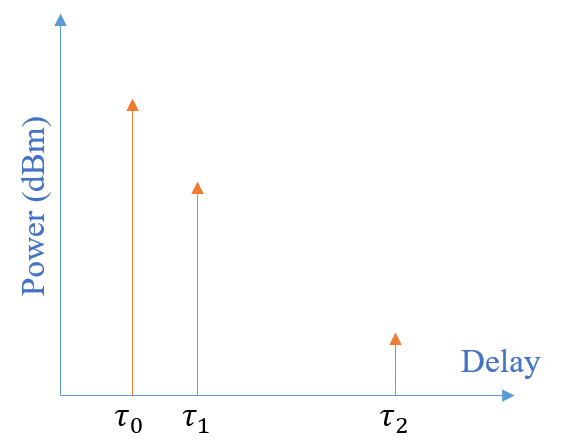
\includegraphics[scale=0.85]
		{pics/PDP.png}
		\caption{PDP pada \textit{multipath fading channel}.}
	\label{fig:PDP}
\end{figure}
\textit{Power Delay Profile} (PDP) merepresentasikan daya rata-rata sebagai fungsi \textit{delay} propagasi akibat \textit{multipath delay} yang dialami kanal. Daya yang diterima dan dispersifitas \textit{multipath} dalam saluran nirkabel dapat diprediksi berdasarkan nilai PDP. Kanal dapa mengalami \textit{multipath} akibat adanya refleksi (\textit{reflection}), pembiasan (\textit{refraction}), hamburan (\textit{scattering}), dan penyaluran (\textit{ducting}) sehingga menyebabkan interferensi \cite{pdp2}. Kanal \textit{multipath} menyebabkan adanya \textit{Inter-Symbol Interference} (ISI) yang dihasilkan dari pengaruh lingkungan jalur rambat antara pemancar dan penerima \cite{pdp1}. 

Dalam proses mengeplot PDP, sumbu $X$ mewakili \textit{delay} propagasi masing-masing \textit{path} dan sumbu $Y$ mewakili daya sinyal dari setiap \textit{path}. Gambar \ref{fig:PDP} menunjukkan contoh bagaimana sinyal yang ditransmisikan akan diterima pada sisi penerima dengan daya yang berbeda-beda melalui kanal \textit{multipath} berdasarkan \textit{delay} propagasi yang berbeda pula. PDP dicirikan dengan nilai \textit{maximum excess delay}, \textit{mean excess delay}, dan \textit{root mean square} (RMS) \textit{delay spread}.
%
%PDP atau \textit{multipath intensity profile} ($A_{c}(\tau)$) adalah daya di \textit{receiver} yang telah dipengaruhi oleh \textit{delay} dan perubahan fasa akibat dari \textit{multipath channel} \cite{pdp1}. \textit{Multipath channel} menyebabkan adanya \textit{Inter-Symbol Interference} (ISI) yang dihasilkan dari pengaruh lingkungan jalur rambat antara pemancar dan penerima. PDP digambarkan dalam grafik daya sinyal untuk setiap \textit{multipath} tergantung dari setiap \textit{propagation delays}-nya. Gambar \ref{fig:PDP} menunjukkan daya sinyal yang diterima di \textit{receiver} memiliki nilai berbeda dalam sebuah \textit{multipath channel} dengan propagation delays ($\tau_{0}, \tau_{1}, \tau_{2}$).     
%\begin{equation}
%p(\tau) = \int_{-\infty }^{\infty } S(f,\tau) df,
%\label{pdp}
%\end{equation}
 	
%\subsection{Pemodelan Kanal Indonesia}
%Model kanal Indonesia didapatkan melalui pengujian kondisi parameter lingkungan Indonesia. Untuk studi awal, representasi dari Indonesia menggunakan parameter lingkungan dari Kota Bandung \cite{ch1}. Keakuratan kanal model Indonesia bisa ditingkatkan dengan menambah sampel dari berbagai kota di Indonesia. Parameter lingkungan seperti tekanan udara, kelembapan, dan suhu yang didapat dari Badan Meteorologi Klimatologi, dan Geofisika (BMKG). Pemodelan kanal dapat menggunakan \textit{software} \textit{New York University Wireless Simulator} (NYUSIM) \text{dengan} parameter dari data rata-rata harian sehingga diharapkan dapat menghasilkan model kanal yang akurat. Kanal model di Kota Bandung dapat direpresentasikan sebagai \textit{multipath fading channel} yang memiliki 18~\textit{paths} dengan \textit{delay interval} 10~ns dan \textit{outage performance} Kota Bandung yang telah \text{divalidasi} secara teori. Hasil dari pemodelan kanal Indonesia yang terkhusus di Kota Bandung telah dibuktikan akan memiliki kinerja yang lebih baik dengan menggunakan \textit{channel coding} LDPC \textit{codes} atau Polar \textit{codes} \cite{ch1}.  



\begin{figure}[tb]
	\centering
	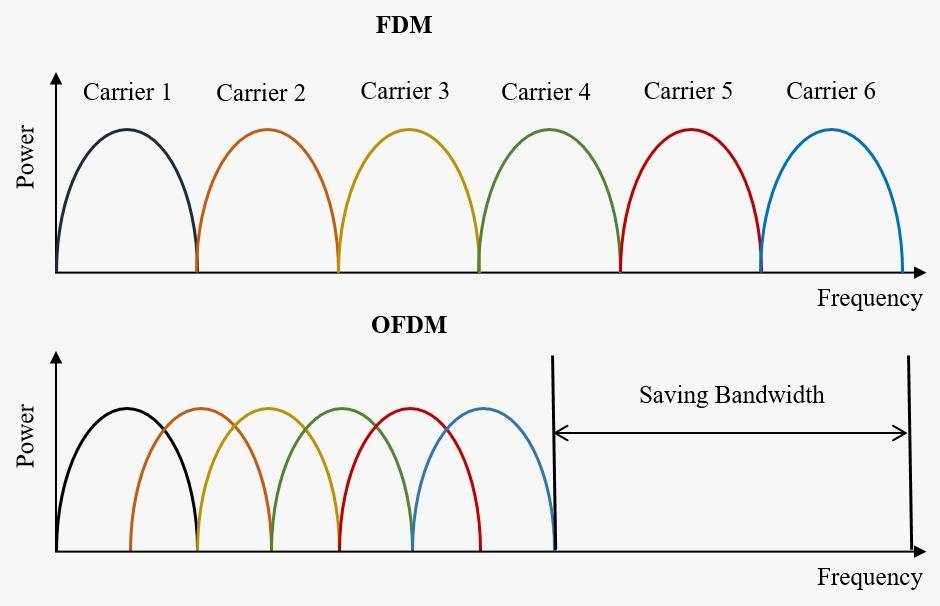
\includegraphics[width=1\textwidth]
	{pics/ofdm}
	\caption{Efisiensi spektrum dengan \textit{saving bandwidth} sebaga hasil OFDM dibandingkan dengan FDM.}
	\label{fig:OFDM}
\end{figure}
\section{\textit{Orthogonal Frequency Division Multiplexing} (OFDM) }
OFDM adalah sebuah skema untuk mengirimkan banyak informasi melalui satu saluran atau \textit{multicarrier modulation} dengan alokasi frekuensi tertentu yang sederhana dan sesuai untuk transmisi data berkecepatan tinggi melalui kanal \textit{multipath fading}. OFDM mampu mengubah kanal \textit{frequency-selective fading} menjadi kanal \textit{frequency-flat fading} dalam sistem transmisi paralel melalui kanal \textit{narrowband} \cite{ofdm}. OFDM mampu menghilangkan gangguan ISI dan \textit{Inter-Carrier Interference} (ICI) melalui penggunaan \textit{cyclic prefix} (CP). OFDM dianggap sebagai penerus teknik \textit{Frequency Division Multiplexing} (FDM) dengan cara menghilangkan ketidakefisienan dalam saluran seperti yang ditunjukkan oleh Gambar \ref{fig:OFDM} dengan memanfaatkan \textit{subcarriers} yang saling tegak lurus (\textit{orthogonal subcarriers}) \cite{ofdm2}.

\begin{figure}[tb]
	\centering
	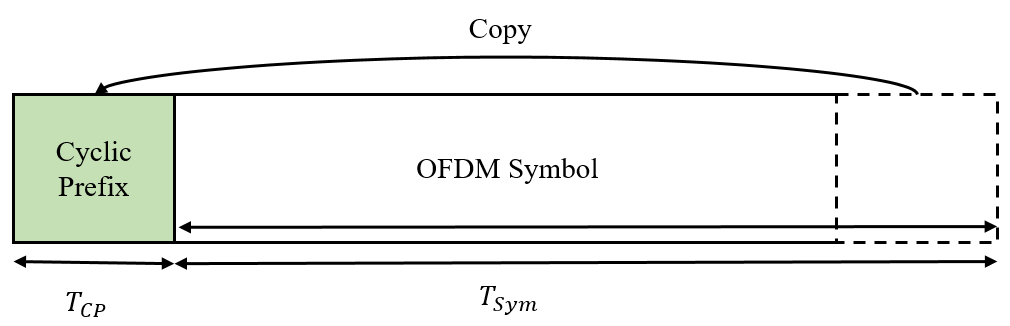
\includegraphics[width=1\textwidth]
	{pics/cyclicprefix}
	\caption{Ilustrasi penambahan CPpada awal OFDM simbol sebesar $T_{CP}$.}
	\label{fig:CP}
\end{figure}


\subsection{\textit{Cyclic Prefix} (CP)}
CP adalah awalan simbol OFDM yang merupakan pengulangan bagian akhir dari simbol OFDM seperti ditunjukkan pada Gambar \ref{fig:CP} dengan $T_{CP}$ adalah panjang CP dan panjang simbol informasi dinyatakan dengan $N$. CP digunakan dalam OFDM untuk mengatasi efek dari ISI akibat kanal \textit{multipath fading}. Simbol yang telah dilengkapi dengan CP akan mampu melakukan \textit{recovery} dengan baik pada sisi penerima walaupun terkena interferensi \textit{fading} dari kanal yang cukup besar. Dalam CP-OFDM, satu blok simbol kompleks dipetakan ke dalam satu pasang \textit{orthogonal carriers}. Arsitektur CP-OFDM memiliki kompleksitas yang rendah, karena penggunaan \textit{Inverse Fast Fourier Transform} (IFFT) dalam OFDM \cite{CP1}. Selain itu, panjang CP diusahakan sama atau lebih besar dari jumlah \textit{path} dalam PDP untuk menjamin kinerja sistem yang terbebas gangguan ISI. Penggunaan CP-OFDM secara umum memiliki dua tujuan, antara lain:
\begin{enumerate}
	\item Pemberian \textit{guard interval} untuk menghilangkan ISI yang disebabkan simbol sebelumnya.
	\item Penyalinan bagian akhir dari simbol yang menyebabkan konvolusi linier dari kanal \textit{frequency-selective fading} dapat dihitung sebagai konvolusi melingkar, sehingga mampu menyederhanakan proses estimasi kanal.
\end{enumerate}

\subsection{\textit{Inverse Fast Fourier Transform} (IFFT) }
IFFT adalah proses untuk menghasilkan simbol-simbol OFDM pada sisi pengirim dengan frekuensi daripada setiap informasinya akan dibuat saling tegak lurus (orthogonal). IFFT mengubah sebuah spektrum, yaitu amplitudo dan fasa dari setiap sinyal informasi ke bentuk sinyal dalam domain waktu \cite{fft}. IFFT mengubah sejumlah simbol bernilai kompleks ke dalam domain waktu dengan jumlah simbol yang tetap. \textit{Subcarrier} yang \textit{orthogonal} pada IFFT digunakan dalam sinyal OFDM agar dapat mengatur amplitudo dan fasa dari setiap simbol dengan mudah.

\subsection{\textit{Fast Fourier Transform} (FFT)}
FFT adalah proses pemisahan antara frekuensi \textit{carrier} dengan simbol OFDM yang diterima pada sisi penerima sebelum didemodulasi dan diubah kembali ke dalam bentuk bit. FFT juga digunakan untuk implementasi \textit{discrete fourier transform} agar lebih cepat dan efisien. Ukuran FFT (FFT \textit{size}) mengacu pada jumlah \textit{subcarrier} dari simbol OFDM yang diharapkan sesuai ukuran $2^N$, dengan $N$ adalah jumlah sampel yang diubah waktu ke domain frekuensi \cite{fft}. Oleh karena itu, ukuran FFT akan mempengaruhi jumlah simbol OFDM untuk setiap blok atau frame dari suatu sistem OFDM. Ukuran FFT ditentukan dengan memperhatikan keseimbangan antara perlindungan terhadap efek \textit{multipath}, pergeseran Doppler (\textit{Doppler shift}), dan kompleksitas sistem. Ukuran FFT yang semakin besar akan mengurangi \textit{subcarrier spacing} dan menambahkan durasi simbol. Hal ini akan memudahkan dalam melindungi simbol OFDM dari interferensi akibat \textit{multipath}. Di sisi lain, berkurangnya \textit{subcarrier spacing} akan membuat sistem lebih terhadap ICI akibat efek Doppler \textit{spread} dalam sistem komunikasi \textit{wireless}. 



\subsection{Matriks \textit{Circulant} dan Matriks \textit{Toeplitz}}
Matriks \textit{circulant} $\mathbf{H}_c$ adalah sebuah matriks \textit{Toeplitz} yang memiliki dimensi mengikuti jumlah CP dan FFT \textit{size}, jumlah baris $\mathbf{H}_c$ dinyatakan oleh
\begin{equation}
	m_{\mathbf{H}_c}=(F+Q \times 2)-1
\end{equation}
dengan $m_{\mathbf{H}_c}$ adalah baris dari $\mathbf{H}_c$, $F$ adalah FFT \textit{size}, dan $Q$ adalah panjang CP. Untuk kolom dari $\mathbf{H}_c$ dinyatakan oleh
\begin{equation}
	n_{\mathbf{H}_c}=F+Q.
\end{equation}

Sifat dari matriks \textit{circulant} yang mudah diturunkan membuat matriks ini dapat digunakan untuk memperkirakan dan menjelaskan perilaku dari matriks \textit{Toeplitz} dengan baik, salah satunya seperti yang terjadi dalam sinyal terima di \textit{receiver} $\mathbf{y}$ yang dinyatakan menurut 
\begin{equation}
\mathbf{y}= \mathbf{H}_c \cdot \mathbf{x}+ \mathbf{n},
\label{matrixeq}
\end{equation} 
dengan $\mathbf{H}_c$ adalah matriks \textit{circulant} yang berisi nilai \textit{path} yang merepresentasikan kondisi kanal. Apabila sebuah kanal memiliki \textit{path} $\mathbf{h}=[~1 ~0.9 ~0.8]$ dan bit yang dikirimkan $\mathbf{x}$ ditambah dengan CP menjadi $\mathbf{x}_{cp}=[c d: a b c d]$, maka sinyal yang diterima dinyatakan menjadi
\begin{equation}
\textbf{y} = \begin{bmatrix}
1   & 0   & 0   & 0   & 0   & 0\\ 
0.9 & 1   & 0   & 0   & 0   & 0\\ 
0.8 & 0.9 & 1   & 0   & 0   & 0\\ 
0   & 0.8 & 0.9 & 1   & 0   & 0\\ 
0   & 0   & 0.8 & 0.9 & 1   & 0\\ 
0   & 0   & 0   & 0.8 & 0.9 & 1\\ 
0   & 0   & 0   &  0  & 0.8 & 0.9\\ 
0   & 0   & 0   &  0  & 0   & 0.8
\end{bmatrix}
\begin{bmatrix}
c\\ 
d\\ 
a\\ 
b\\ 
c\\ 
d
\end{bmatrix}
+ \begin{bmatrix}
n_{1}\\ 
n_{2}\\ 
n_{3}\\ 
n_{4}\\ 
n_{5}\\ 
n_{6}\\ 
n_{7}\\ 
n_{8}
\end{bmatrix}~,\\
\end{equation}



%\begin{equation}
%H=\begin{bmatrix}  
%\tikzmarknode{m1}{c}\\ 
%\tikzmarknode{m3}{0.9c + d} \\ 
%0.8c + 0.9d + a \\ 
%0.8d + 0.9a + b\\ 
%0.8a + 0.9b + c \\ 
%0.8b + 0.9c + d\\ 
%\tikzmarknode{m2}{0.8c + 0.9d}\\ 
%\tikzmarknode{m4}{0.8d}
%\end{bmatrix}
%\end{equation}




\begin{equation}
\mathbf{y} = \begin{bmatrix}
\tikzmarknode{m1}{c}\\ 
\tikzmarknode{m3}{0.9c + d} \\ 
0.8c + 0.9d + a \\ 
0.8d + 0.9a + b\\ 
0.8a + 0.9b + c \\ 
0.8b + 0.9c + d\\ 
\tikzmarknode{m2}{0.8c + 0.9d}\\ 
\tikzmarknode{m4}{0.8d}
\end{bmatrix}
+ \begin{bmatrix}
\tikzmarknode{n1}{n_{1}}\\ 
\tikzmarknode{n3}{n_{2}}\\ 
n_{3}\\ 
n_{4}\\ 
n_{5}\\ 
n_{6}\\ 
\tikzmarknode{n2}{n_{7}}\\ 
\tikzmarknode{n4}{n_{8}}
\end{bmatrix}~,
\end{equation}  
\AddToShipoutPictureBG{%
	\begin{tikzpicture}[overlay,remember picture]
	\node[fill=gray!70,rounded corners,fit=(m1)(m3)]{};
	\node[fill=gray!70,rounded corners,fit=(m2)(m4)]{};
	\node[fill=gray!70,rounded corners,fit=(n1)(n3)]{};
	\node[fill=gray!70,rounded corners,fit=(n2)(n4)]{};
	%	\node[fill=purple!60,inner xsep=1.6ex,rounded corners,fit=(m2)(m3)]{};
	\end{tikzpicture}
}
Setelah CP dihapus dengan menghapus bagian yang berwarna abu-abu, sinyal yang diterima menjadi 
\begin{equation}
\mathbf{y} = \begin{bmatrix} 
0.8c + 0.9d + a \\ 
0.8d + 0.9a + b\\ 
0.8a + 0.9b + c \\ 
0.8b + 0.9c + d\\ 
\end{bmatrix}
+ \begin{bmatrix}
n_{3}\\ 
n_{4}\\ 
n_{5}\\ 
n_{6}\\ 
\end{bmatrix}~, \\ 
\end{equation}
yang ekivalen dengan
\begin{eqnarray}
\mathbf{y} &=&  \begin{bmatrix}
1   & 0    & 0.8   & 0.9 \\ 
0.9 & 1   & 0   & 0.8    \\ 
0.8 & 0.9 & 1   & 0     \\ 
0   & 0.8 & 0.9 & 1     \\ 
\end{bmatrix}
\begin{bmatrix}
a\\ 
b\\ 
c\\ 
d 
\end{bmatrix}
+ \begin{bmatrix}
n_{1}\\ 
n_{2}\\ 
n_{3}\\ 
n_{4}
\end{bmatrix}~,\\
&=& \mathbf{H}_c\cdot \mathbf{x} + \mathbf{n}.
\end{eqnarray}


\section{\textit{Signal-to-Noise Power Ratio} (SNR)}
\textit{Signal-to-Noise Power Ratio} (SNR) adalah rasio antara amplitudo sinyal data yang diinginkan $P_{signal}$ dan amplitudo \textit{noise} $P_{noise}$ dalam kanal tranmisi pada waktu tertentu. SNR digunakan untuk mengukur kualitas sebuah kanal transmisi. Apabila SNR semakin tinggi, maka semakin mudah juga untuk mengidentifikasi dan mengisolasi sumber \textit{noise} pada kanal. SNR bernilai nol menunjukkan bahwa sinyal data hampir tidak dapat dibedakan dari \textit{noise} yang ada. Penurunan SNR juga berpengaruh pada penurunan \textit{throughput} yang disebabkan oleh kesalahan yang terjadi di beberapa paket data \cite{SNR}. SNR $\gamma$ biasanya dinyatakan secara logaritmik dalam desibel (dB) menurut
\begin{figure}[b!]
	\centering	
	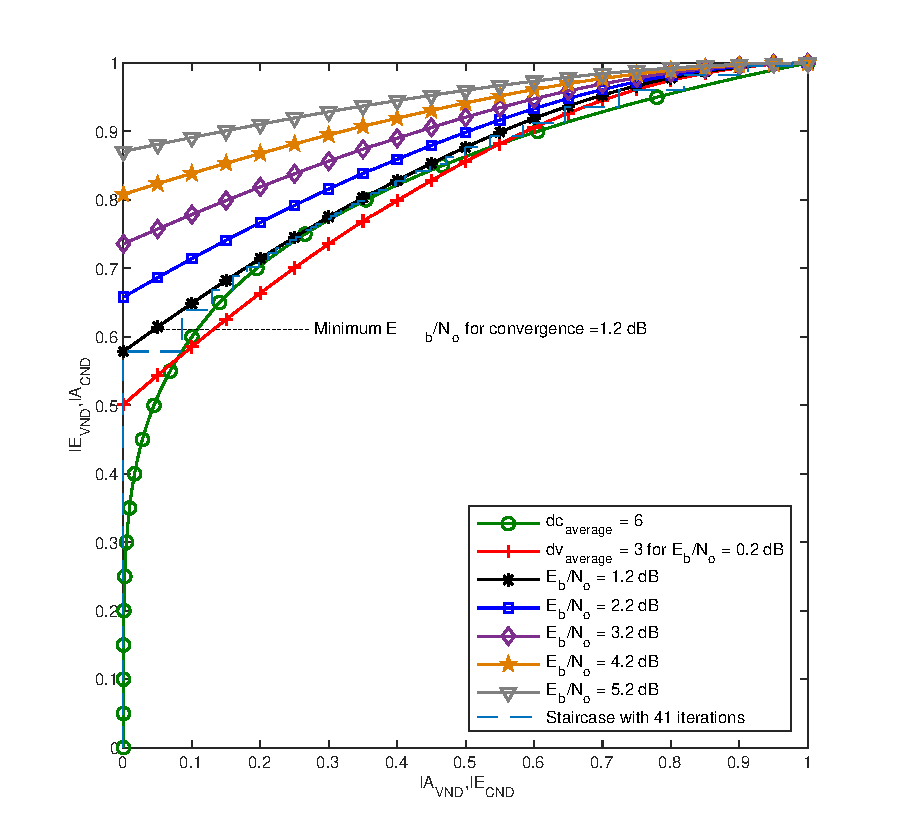
\includegraphics[width=1\textwidth]
	{pics/exit.pdf}
	\caption{EXIT \textit{chart} LDPC \textit{codes} untuk $d_{v}=3$ dan $d_{c}=6$ pada berbagai $E_b/N_0$.}
	\label{fig:EXIT chart}
\end{figure}
\begin{equation}
	\gamma = \frac{P_{signal}}{P_{noise}}.
\end{equation}

%-----------------------------------------------------------------------------%

\section{\textit{Extrinsic Information Transfer} (EXIT) \textit{Chart} }

EXIT \textit{chart} pertama diperkenalkan oleh Stephan ten Brink untuk menganalisis informasi timbal balik di \textit{decoder} dengan menggunakan proses \textit{iterative} dan untuk mengetahui jumlah iterasi yang diperlukan agar \textit{decoding} sukses \cite{exit23}. Proses dari transfer informasi direpresentasikan dalam bentuk grafik. Informasi yang masuk \textit{decoder} atau belum di-\textit{decode} disebut \textit{apriori mutual information} ($I_{A}$), sedangkan informasi yang keluar dari \textit{decoder} atau telah di-\textit{decode} disebut \textit{extrinsic mutual information} ($I_{E}$). EXIT \textit{chart} menganalisis menggunakan dua \textit{decoder} dan keluaran \textit{decoder} pertama adalah masukan \textit{decoder} kedua. Lalu di iterasi kedua, keluaran \textit{decoder} kedua menjadi masukan \textit{decoder} pertama dan begitu seterusnya. EXIT \textit{chart} direpresentasikan menggunakan grafik dengan mengeplot kinerja kedua \textit{decoder} dengan sumbu yang saling berlawanan. Kurva yang dihasilkan menggunakan fungsi \textit{staircase} yang dimulai dari titik ($0,0$) ketika tidak ada informasi timbal balik dan \textit{decoding} berhasil ketika mencapai titik ($1,1$) seperti pada Gambar \ref{fig:EXIT chart}. 		\ClearShipoutPicture

\begin{figure}[t!]

	\centering
	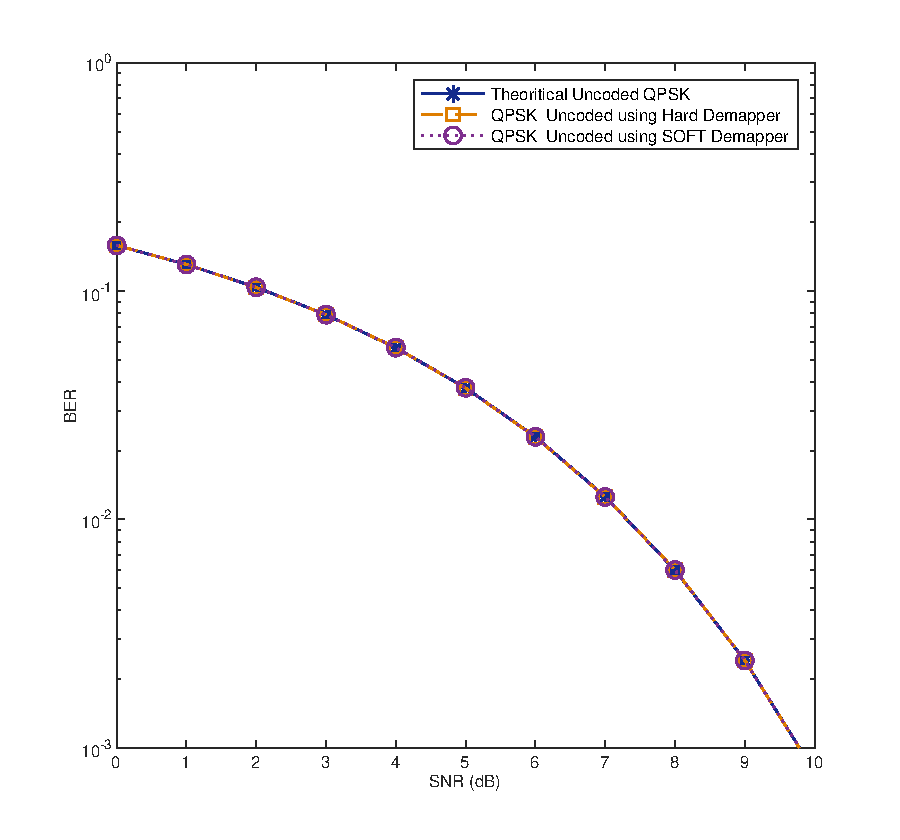
\includegraphics[width=1\textwidth]
	{pics/uncoded.pdf}
	\caption{Kinerja BER \textit{Uncoded} BER QPSK pada kanal AWGN dibandingkan dengan BER teori QPSK.}
	\label{fig:BER}

\end{figure}

\section{\textit{Bit Error Rate} (BER)}
Saat ini, segala komunikasi telah beralih ke bentuk komunikasi digital. Salah satu parameter pengukuran kinerja dari komunikasi digital menggunakan BER. Nilai BER didapat dari membandingkan bit yang diterima dengan bit yang ditransmisikan di sebuah sistem elektronika, antena, dan \textit{signal path} \cite{ber1}. Untuk di kanal AWGN, BER adalah kinerja yang dipengaruhi langsung oleh \textit{noise channel} dan untuk di \textit{fading channel} BER akan menjadi lebih buruk \cite{ber2}.
Persamaan sederhana BER adalah
\begin{equation}
BER=\frac{jumlah \; bit \; error}{total \; bit \; yang \; dikirimkan}.
\label{eq: Persamaan BER sederhana}
\end{equation} % From here on no logo
Perhitungan BER dalam teori tersebut untuk modulasi QPSK pada kanal AWGN dinyatakan oleh
\begin{equation}
BER_{QPSK\_AWGN}=\frac{1}{2} \mathrm{erfc} \left(  \sqrt{\frac{\gamma}{2} }  \right)
\end{equation}
dengan $\gamma$ adalah SNR. BER teori untuk modulasi QPSK pada kanal \textit{singlepath} dinyatakan dengan 
\begin{equation}
BER_{QPSK-Fading}= \frac{1}{2}\left [ 1-\frac{1}{\sqrt{1+\frac{2}{\gamma}}} \right ].
\end{equation} 

%\section{\textit{Bit Error Rate} (BER)}
%\begin{figure}[tb]
%\centering
%	\includegraphics[scale=0.52]
%		{pics/jadin.png}
%		\caption{Nilai \textit{Uncoded} BER QPSK pada AWGN \textit{channel}.}
%	\label{fig:BER}
%\end{figure}
%Saat ini, segala komunikasi telah beralih ke bentuk komunikasi digital. Salah satu parameter pengukuran kinerja dari komunikasi digital menggunakan BER. Nilai BER didapat dari membandingkan bit yang diterima dengan bit yang ditransmisikan di sebuah sistem elektronika, antena, dan \textit{signal path} \cite{ber1}. Untuk di  AWGN \textit{channel}, BER adalah kinerja yang dipengaruhi langsung oleh \textit{noise channel} dan untuk di \textit{fading channel} BER akan menjadi lebih buruk \cite{ber2}.
%Persamaan sederhana BER adalah
%\begin{equation}
%BER=\frac{jumlah \; bit \; error}{total \; bit \; yang \; dikirimkan}.
%\label{eq: Persamaan BER sederhana}
%\end{equation}
% 
%\textit{Noise} merupakan parameter yang mempengaruhi terjadinya BER, contoh penyebab terjadinya \textit{noise} adalah \textit{fading} dan pengaruh suhu alat. Pada AWGN \textit{channel}, \textit{noise} direpresentasikan dalam bentuk distribusi \textit{Gaussian}, sedangkan pada \textit{fading channel}, \textit{noise} direpresentasikan dalam distribusi \textit{Rayleigh} atau \textit{Ricean}. Berdasarkan dari fasa dan frekuensi pembawa, BER dapat didefinisikan sebagai berikut
%\begin{equation}
%P_{b}=\frac{2(1-\frac{1}{L})}{\log_{2}L}Q\left [ \sqrt{\left ( \frac{3\log_{2}L}{L^{2}-1} \right )} \frac{2E_{b}}{N_{o}} \right ],
%\label{eq: Rumus BER}
%\end{equation} 
%dengan nilai $L$ adalah jumlah \textit{level} di setiap dimensi dari \textit{M-ary} sistem modulasi, $E_{b}$ adalah energi setiap bit, dan $\frac{N_{0}}{2}$ adalah rapat daya \textit{noise}.


  
   


	% Bab 3 : Perancangan
%-----------------------------------------------------------------------------%
\chapter{\babTiga}
%-----------------------------------------------------------------------------%
Bab ini membahas tentang perancangan dan pemodelan sistem LDPC \textit{codes} DVB-T2 mulai dari \textit{transmitter}, model kanal, hingga \textit{receiver}, juga letak LDPC \textit{codes} dalam sistem tersebut. Bab ini juga mengusulkan \textit{degree distribution} LDPC \textit{codes} DVB-T2, serta teknik untuk menghitung \textit{girth} pada LDPC \textit{codes} dan merancang LDPC \textit{codes} tanpa adanya \textit{girth} 4.
%alir dan model sistem mulai dari \textit{transmitter}, model kanal, hingga \textit{receiver}, juga posisi LDPC \textit{codes} dalam sistem tersebut.

\begin{figure}[tb]
%	\hspace{-6cm}
	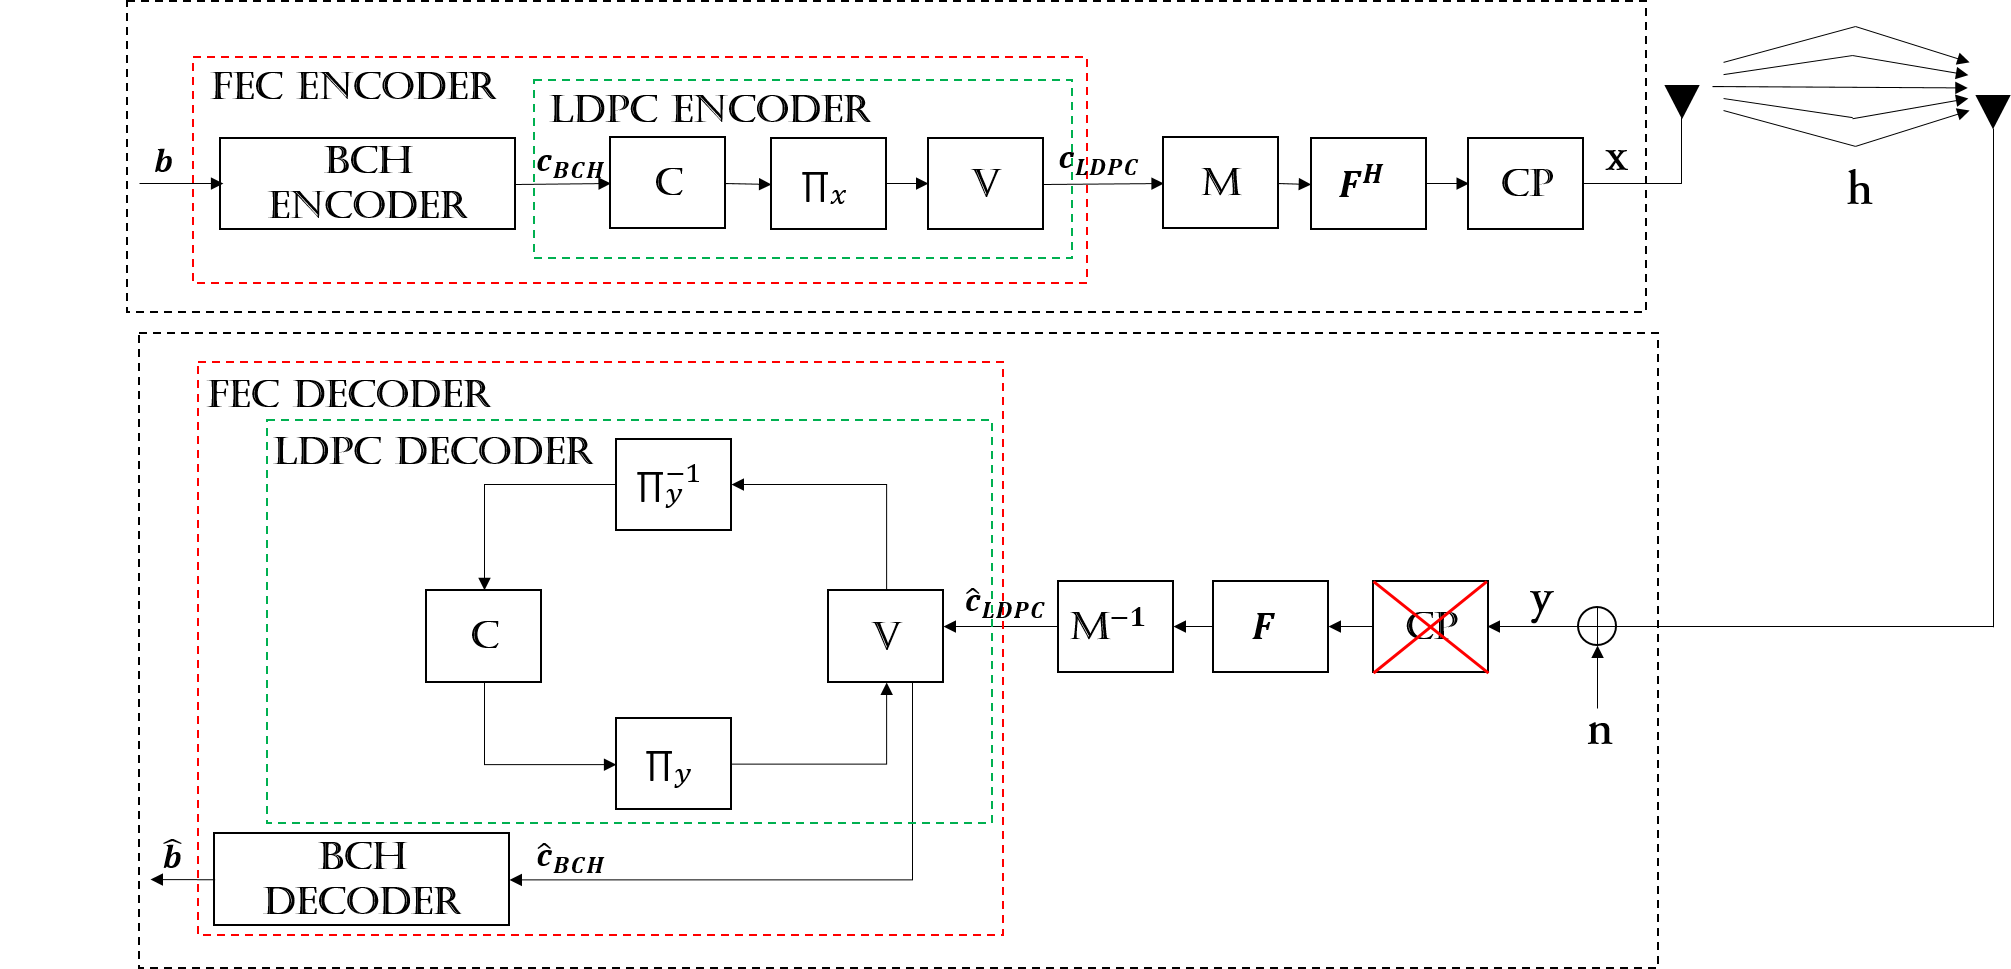
\includegraphics[scale=0.4]
	{pics/sistemmo.png}
	\caption{Diagram blok sistem transmisi DVB-T2 dengan penekanan pada LDPC \textit{codes}.}
	\label{fig:sistem model}
\end{figure}

\begin{figure}[tb]
	\centering
	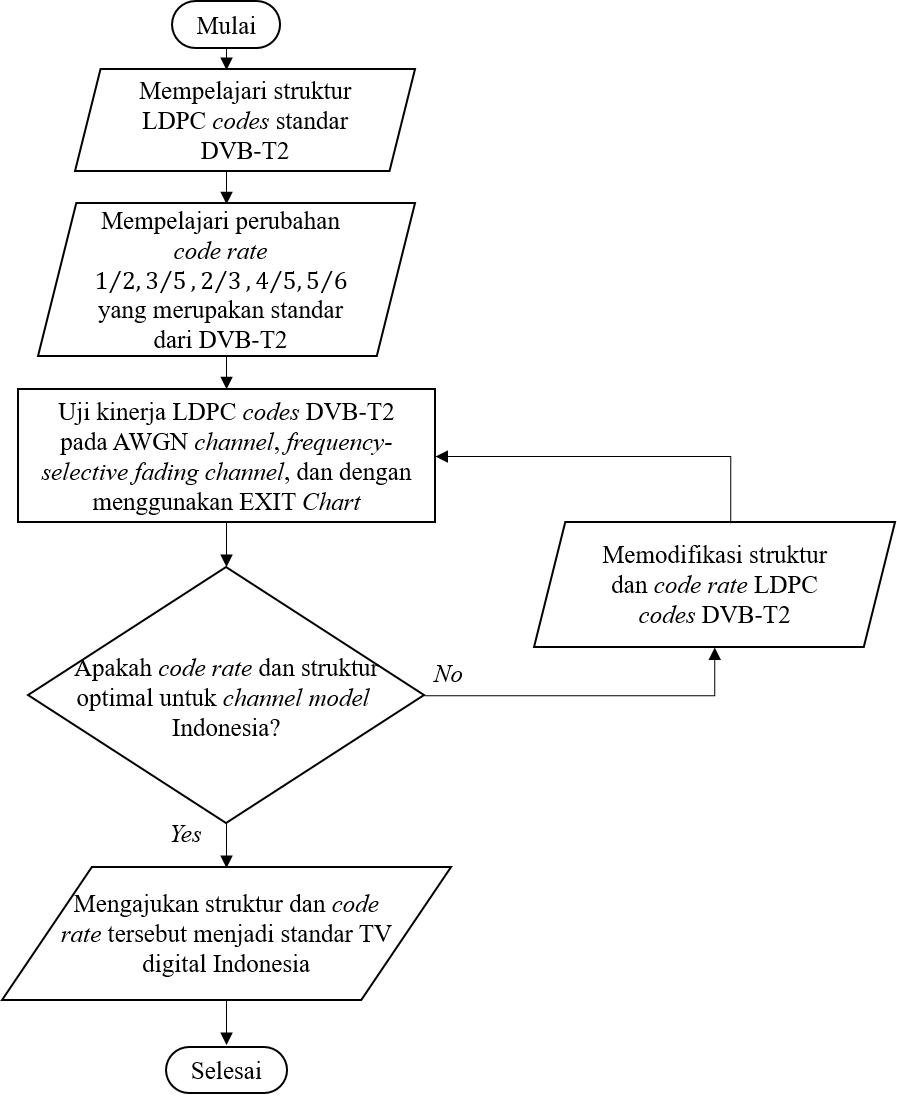
\includegraphics[scale=0.8]
		{pics/diagram/alir.png}
		\caption{Diagram alir evaluasi kinerja LDPC \textit{codes} pada sistem DVB-T2.}
	\label{fig:Diagram Alir}
\end{figure}








%Setelah memahami struktur dari LDPC \textit{codes} DVB-T2, dapat diketahui jika struktur dari LDPC \textit{codes} akan dipengaruhi oleh \textit{code rate} yang digunakan. DVB-T2 memiliki nilai \textit{code rate}: $\frac{1}{2}, \frac{3}{5}, \frac{2}{3}, \frac{3}{4}, \frac{4}{5},$ atau $\frac{5}{6}$ pada standar TS 102 831. Kemudian dilanjutkan dengan mempelajari perubahan yang terjadi dalam penggunaan setiap \textit{code rate} tertenru terhadap struktur dari LDPC \textit{codes}. Berikutnya dilakukan pengujian dan pengamatan kinerja LDPC \textit{codes} dari setiap \textit{code rate} dalam sebuah proses pengiriman data yang menggunakan pemodelan kanal AWGN \textit{Channel} dan \textit{frequency selective fading channel}. Pada langkah selanjutnya, menggunakan EXIT \textit{Chart} untuk menganalisis dan mengoptimalisasi kinerja LDPC \textit{codes} DVB-T2. Apabila hasil dari analisis kinerja LDPC \textit{codes} DVB-T2 yang didapat memiliki kinerja optimal di kondisi alam Indonesia, maka struktur dan \textit{code rate} yang didapat akan diajukan menjadi standar TV digital Indonesia. Namun, apabila LDPC \textit{codes} DVB-T2 memiliki kinerja yang tidak optimal di kondisi alam Indonesia, maka langkah selanjutnya perlu memodifikasi struktur dan \textit{code rate} LDPC \textit{codes} DVB-T2 sehingga dapat bekerja dengan baik dan optimal di kondisi alam Indonesia. 
%-----------------------------------------------------------------------------%
\section{Blok Sistem DVB-T2}
%-----------------------------------------------------------------------------%

%C (CND) V (VND) 
Diagram blok sistem pada Gambar \ref{fig:sistem model} menunjukkan sistem DVB-T2 dari \text{pengirim} ($Tx$) hingga ke penerima ($Rx$) yang berfungsi untuk mempermudah dalam menjelaskan alur komunikasi data DVB-T2. Dimulai dari sisi pengirim, bit informasi $\mathbf{b}$ dibangkitkan secara acak dengan probabilitas kemunculan bit 0 dan 1 sama. Bit yang telah dibangkitkan kemudian masuk ke FEC \textit{encoder}, $\mathbf{b}$ yang masuk ke BCH \textit{encoder} merupakan \textit{outer code} FEC DVB-T2. Setelah itu dari proses BCH \textit{encoder} menghasilkan \textit{codeword} BCH ($\mathbf{c}_{BCH}$) dan akan masuk ke LDPC \textit{encoder} yang merupakan \textit{inner code} FEC DVB-T2. Bit akan di-\textit{encode} oleh Blok C ke Blok V dengan Blok $\Pi_{x}$, sehingga menghasilkan \textit{codeword} ($\mathbf{c}_{LDPC}$). 

Blok C merupakan deretan CND dan Blok V merupakan deretan VND. Blok \textit{Bit Interleaver} ($\Pi_{x}$) mengatur ulang bit, sehingga hasil keluaran dapat dibaca dalam siklus bolak-balik. Kemudian, hasil keluaran dipetakan ke modulasi QPSK yang ditunjukkan dengan Blok $M$, sehingga menghasilkan data berupa simbol per-bit. Simbol akan dikirimkan dengan mode transmisi \textit{orthogonal multi-carrier} yang selanjutnya simbol akan ditransformasikan dari domain frekuensi ke domain waktu pada Blok FFT ($F^{H}$). Blok $F^{H}$ juga berfungsi sebagai OFDM \textit{baseband modulator} yang akan memodulasi frekuensi \textit{subcarrier} untuk setiap simbol yang dibangkitkan pada blok ini. Simbol akan ditambahkan CP untuk mempertahankan \text{properti} ortogonalitas sinyal dan mencegah terjadinya ISI dan ICI. Berikutnya, data akan dikirimkan melalui antena dan melewati kanal \textit{multipath}.

Sinyal terima berupa data yang telah terpengaruhi oleh kanal \textit{multipath} dan \textit{noise}. Kemudian, CP pada sinyal OFDM yang diterima akan dilepas dan sinyal terima akan ditransformasikan kembali dari domain waktu ke domain frekuensi di Blok $F$. Lalu, sinyal terima dikembalikan menjadi bit-bit data pada Blok \textit{Demodulator} ($M^{-1}$) menjadi bit $\hat{\mathbf{c}}_{LDPC}$. Bit $\hat{\mathbf{c}}_{LDPC}$ akan di-\textit{decode} oleh LDPC \textit{decoder} di bagian FEC \textit{decoder}. Proses \textit{iterative decoding} di LDPC \textit{decoder} dilakukan oleh Blok $V$, Blok Bit \textit{Deinterleaver} ($\Pi^{-1}_{y}$), Blok $C$, dan Blok $\Pi_{y}$. Proses \textit{decoding} LDPC \textit{codes} menggunakan SPA, sehingga pada Blok $V$ LLR diproses dengan persamaan 
%Nilai $d_{v}$ adalah jumlah banyak node yang terhubung ke VND,  
\begin{equation}
L_{E_{{v_{i}}}}(n)=L_{ch}+\sum_{j=1,j\neq i}^{d_{v_{n}}} L_{A_{v_{j}}},
\end{equation}
dan pada Blok $C$ 
\begin{equation}
L_{E_{{c_{j}}}}(k)=\sum_{i=1,i\neq j}^{d_{c_{k}}} \boxplus L_{A_{c_{i}}},
\end{equation}
\begin{gather}
L_{E_{c_{j}}}(k)=\sum_{i=1,i\neq j}^{d_{c_{k}}}\boxplus L_{A_{c_{i}}},\\
\approx  (-1) sgn \left \{  L_{A_{c_{i}}} \right \} sgn \left \{ L_{A_{c_{i+1}}} \right \} \cdot \min \left \{ \left | L_{A_{c_{i}}} \right |,\left | 
L_{A_{c_{i+1}}} \right | \right \}.
\end{gather}
%dengan $\Lambda (\theta_{1} ) \boxplus \Lambda (\theta_{2} )$ adalah  
%\begin{eqnarray}
%\Lambda (\theta_{1} ) \boxplus \Lambda (\theta_{2} ) = \ln\frac{e^{\Lambda (\theta _{1})}+e^{\Lambda (\theta _{2})}}{1+e^{\Lambda(\theta_{1})}e^{\Lambda(\theta_{2})}}, \\
%\approx (-1) \mathrm{sgn}\left \{ \Lambda(\theta_{1}) \right \} \mathrm{sgn} \left \{ \Lambda(\theta_{2}) \right \}\cdot \mathrm{min} \left \{ \left | \Lambda(\theta_{1})  \right |, \left | \Lambda(\theta_{2})  \right | \right \}.
%\end{eqnarray}
Setelah proses LDPC \textit{decoding} yang menghasilkan \textit{codeword} BCH \textit{codes} ($\hat{\mathbf{c}}_{BCH}$), $\hat{\mathbf{c}}_{BCH}$ akan masuk ke BCH \textit{decoder} untuk menghasilkan bit informasi ($\hat{\mathbf{b}}$). Bit informasi yang diterima akan dibandingkan dengan bit kirim untuk dianalisis.

\section{Skenario Pengujian Kinerja LDPC \textit{Codes} DVB-T2}
Setiap LDPC \textit{codes} yang terbentuk dari setiap nilai \textit{code rate} akan diuji kinerja BER-nya dan akan dioptimalisasi dengan EXIT \textit{chart} untuk mendapatkan \textit{code rate} dan struktur  LDPC \textit{codes} sehingga dapat bekerja optimal di \textit{channel model} DVB-T2 Indonesia. Apabila kinerja LDPC \textit{codes} dari standar DVB-T2 memiliki kinerja optimal di \textit{channel model} DVB-T2 Indonesia, maka struktur dan \textit{code rate} yang didapat akan diajukan menjadi standar TV digital Indonesia. Namun, apabila LDPC \textit{codes} dari standar DVB-T2 memiliki kinerja yang tidak optimal di \textit{channel model} DVB-T2 Indonesia, maka langkah selanjutnya perlu memodifikasi struktur dan \textit{code rate} LDPC \textit{codes} DVB-T2, sehingga dapat bekerja dengan baik dan optimal pada \textit{channel model} DVB-T2 Indonesia. 
%-----------------------------------------------------------------------------%
%\section{Skenario Pengujian Sistem}
%-----------------------------------------------------------------------------%
%Merujuk ke Tobias Oetiker \cite{tobi_latex}, Tex adalah sebuah program komputer yang dibuat oleh Donald E. Knuth.
%Pengujian sistem dimulai dengan  mempelajari dan memahami struktur standar LDPC \textit{codes} DVB-T2 yang ditunjukkan pada Gambar \ref{fig:Diagram Alir}. 
%\section{Struktur LDPC \textit{Codes} Standar DVB-T2}
%Sesuai standar, DVB-T2 memiliki dua \textit{channel coding}. LDPC \textit{codes} adalah salah satu \textit{channel coding} yang digunakan sebagai \textit{inner codes} dalam FEC DVB-T2. LDPC \textit{codes} DVB-T2 merupakan \textit{irregular} LDPC \textit{codes}. DVB-T2 memiliki panjang blok 16200 dan 64800. DVB-T2 memiliki \textit{parity check} yang pada bagian informasi menggunakan \textit{cyclic structure} dan di bagian \textit{parity}-nya menggunakan \textit{staircase structure}. 
\section{Perancangan LDPC \textit{Codes} DVB-T2}
LDPC \textit{codes} DVB-T2 dengan panjang blok $N_{LDPC}=16200$ memiliki nilai \textit{code rate} $R_e=\left \{ \frac{4}{9}, \frac{3}{5}, \frac{2}{3}, \frac{11}{15}, \frac{7}{9}, \frac{37}{45} \right \}$. Setiap \textit{code rate} pada LDPC \textit{codes} DVB-T2 memiliki nilai \textit{effective code rate} dan VND untuk setiap \textit{variable nodes} yang telah ditunjukkan oleh Tabel \ref{table:dvb-t2lite}. Perancangan matriks \textit{parity check} LDPC \textit{codes} $\mathbf{H}$ untuk setiap \textit{code rate} menggunakan nilai seperti pada Tabel \ref{table:adressldpc}, sedangkan matriks generator $\mathbf{G}$ dibentuk menggunakan Gauss Jordan \textit{elimination}. Tugas Akhir ini melakukan perancangan LDPC \textit{codes} untuk semua \textit{code rate}. 

Matriks $\mathbf{H}$ yang terbentuk pada LDPC \textit{codes} DVB-T2 dengan $N_{LDPC}=16200$ memenuhi dimensi matriks
\begin{equation}
	(1-R_e) \cdot 16200 \times 16200
\end{equation}
dengan $R$ adalah \textit{code rate}, sehingga setiap \textit{code rate} akan mengirimkan bit informasi ($\mathbf{b}$) sebanyak 
\begin{equation}
	b = R_e \times 16200.
\end{equation}

\section{\textit{Quadrature Phase Shift Keying} (QPSK)}
Dalam standar, DVB-T2 dapat menggunakan modulasi QPSK, 16-QAM, 64-QAM, ataupun 256-QAM. Dalam Tugas Akhir ini DVB-T2 menggunakan modulasi QPSK. QPSK memiliki empat kemungkinan simbol. Setiap simbolnya akan membawa dua bit. Setiap fasa dari QPSK memiliki empat kemungkinan dengan nilai 
\begin{equation}
\varphi (t)=(2i-1)\frac{\pi}{4} \;\;\;\;\;\;\;\;\; i=1,2,3,4, 
\label{eq:fasa QPSK}
\end{equation} 
maka setiap simbolnya memiliki persamaan sebagai berikut: 
\begin{equation}
s_{i}(t)=\sqrt{\frac{2E}{T}}cos\left [ (2i-1)\frac{\pi}{4}\right ] cos\left [ 2\pi f_{c}t \right ]-\sqrt{\frac{2E}{T}}sin\left [ (2i-1)\frac{\pi}{4}\right ]sin\left [ 2\pi f_{c}t \right ]
\label{eq:simbol QPSK}
\end{equation}
dengan $0\leq t\leq T$ dan $i=\{ 1\dots 4 \} $. Setiap simbol memiliki nilai fasa yang ditunjukkan pada Tabel \ref{tab:QPSK}.
\begin{table}
	\centering
	\caption{Pemetaan simbol QPSK yang dipakai dalam Tugas Akhir ini.}
	\begin{tabular}{|c|c|lll}
		\cline{1-2}
		Bit informasi & Simbol QPSK \\ \cline{1-2}
		00            &   $\frac{\pi}{4}$  \\ \cline{1-2}
		10            &   $\frac{3\pi}{4}$  \\ \cline{1-2}
		11            &   $\frac{5\pi}{4}$   \\ \cline{1-2}
		01            &   $\frac{7\pi}{4}$    \\ \cline{1-2}
	\end{tabular}
	\label{tab:QPSK}
\end{table}


%DVB-T2 dapat memiliki nilai \textit{code rate}: $\frac{1}{2}, \frac{3}{5}, \frac{2}{3}, \frac{3}{4}, \frac{4}{5},$ atau $\frac{5}{6}$. Nilai-nilai \textit{code rate} tersebut telah ditetapkan oleh standar TS 102.831. Setiap nilai \textit{code rate} akan mempengaruhi bentuk dari LDPC \textit{codes}. Nilai \textit{code rate} terkecil atau $\frac{1}{2}$ memiliki perlindungan proteksi maksimal dan laju data minimal, sedangkan untuk \textit{code rate} terbesar atau $\frac{5}{6}$ memiliki perlindungan proteksi minimal dan laju data maksimal. Dapat diketahui bahwa jika kanal sempurna, maka semakin besar nilai \textit{code rate} akan memiliki laju data yang semakin cepat. Nilai \textit{code rate} sendiri didapatkan dari berbandingan matriks bagian informasi dengan total matriks, sehingga nilai \textit{code rate} akan mempengaruhi matriks LDPC \textit{codes}. Matriks LDPC \textit{codes} terdiri dari bagian informasi dan \textit{parity}, besar keduanya dipengaruhi oleh nilai \textit{code rate} dari LDPC \textit{codes}. 
%\section{Pemodelan Kanal}
%LDPC \textit{codes} akan diuji pada AWGN \textit{channel} dan \textit{frequency selective fading channel} dengan menggunakan \textit{channel model} DVB-T2 di wilayah Indonesia.
%Kondisi probabilitas bersyarat pada sinyal terima, jika yang dikirimkan adalah QPSK
%\begin{equation}
%p(r_{x}\mid t_{x}=+1)=\frac{1}{\sigma \sqrt{2\pi}}\cdot \exp \left ( \frac{\left ( y-1 \right )^{2}}{2\sigma ^{2}} \right ),
%\end{equation}
%\begin{equation}
%p(r_{x}\mid t_{x}=-1)=\frac{1}{\sigma \sqrt{2\pi}}\cdot \exp \left ( \frac{\left ( y+1 \right )^{2}}{2\sigma ^{2}} \right ).
%\end{equation} 
\section{\textit{Channel Model} DVB-T2 Indonesia }
Tugas Akhir ini mensimulasikan proses transmisi \textit{broadband} pada \textit{channel model} DVB-T2 Indonesia berdasarkan \cite{pdpband}, \textit{channel model} DVB-T2 di daerah Bandung digunakan sebagai representasi dari Indonesia.  PDP didapatkan melalui New York \textit{channel simulator} (NYUSIM) dengan menggunakan parameter dari Kota Bandung dan DVB-T2. \textit{Channel model} DVB-T2 pada daerah Bandung mengalamai \textit{frequency selective fading channel}, kondisi yang terjadi saat \textit{bandwidth} kanal lebih kecil daripada \textit{bandwidth} sinyal transmisi. Akibatnya kanal akan mengalami \textit{multipath} dan ISI. Setelah proses normalisasi \textit{channel model} DVB-T2 Bandung menghasilkan \textit{path} sebanyak 8 \textit{path} melalaui NYUSIM. Untuk mengurangi efek dari \textit{frequency selective fading channel} dan \textit{multipath}, DVB-T2 menggunakan OFDM.


\section{\textit{Soft Decoding}}
\textit{Soft decoding} menggunakan \textit{Log-Likehood Ratio} (LLR), LLR merupakan pengukuran statistik untuk membandingkan dua model statistik. LLR membandingkan antar probabilitas pada $p(v)=0$ dan $p(v)=1$. LLR pada sinyal terima $y$ dapat dihitung dengan
\begin{eqnarray}
LLR &=& \log\frac{P\left ( y\mid x=+1 \right )}{P\left ( y\mid x=-1   \right )}, \nonumber \\
LLR &=& \frac{2}{\sigma ^2}\cdot y
\end{eqnarray}
dengan $\sigma$ adalah variansi untuk \textit{double-sided noise} dengan distribusi Gaussian.
% 
%Tugas Akhir ini mengasumsikan komunikasi nirkabel TV digital dengan transmisi \textit{broadband}, maka dari itu \textit{frequency selective fading channel} diajukan sebagai pemodelan kanalnya. \textit{Frequency selective fading channel} adalah kondisi saat \textit{bandwidth} kanal lebih kecil daripada \textit{bandwidth} sinyal transmisi, akibatnya kanal akan menghasilkan \textit{multipath} dan ISI. Model matematika \textit{frequency selective fading channel} 
%\begin{equation}
%Y(f)=X(f)H(f)+N(f),
%\end{equation}
%dengan $X(f)$ didefinisikan sebagai sinyal yang dikirimkan dalam \textit{domain} frekuensi, $H(f)$ sebagai respon frekuensi dari kanal, $N(f)$ sebagai \textit{noise thermal} yang terdistribusi Gaussian, dan $Y(f)$ sebagai sinyal diterima dalam \textit{domain} frekuensi.  
%\begin{figure}[tb]
%\centering
%	\includegraphics[scale=0.62]
%		{pics/kon.png}
%		\caption{Diagram konstelasi QPSK.}
%	\label{fig:BER}
%\end{figure}



 \begin{figure}[tb]
	
	\centering
	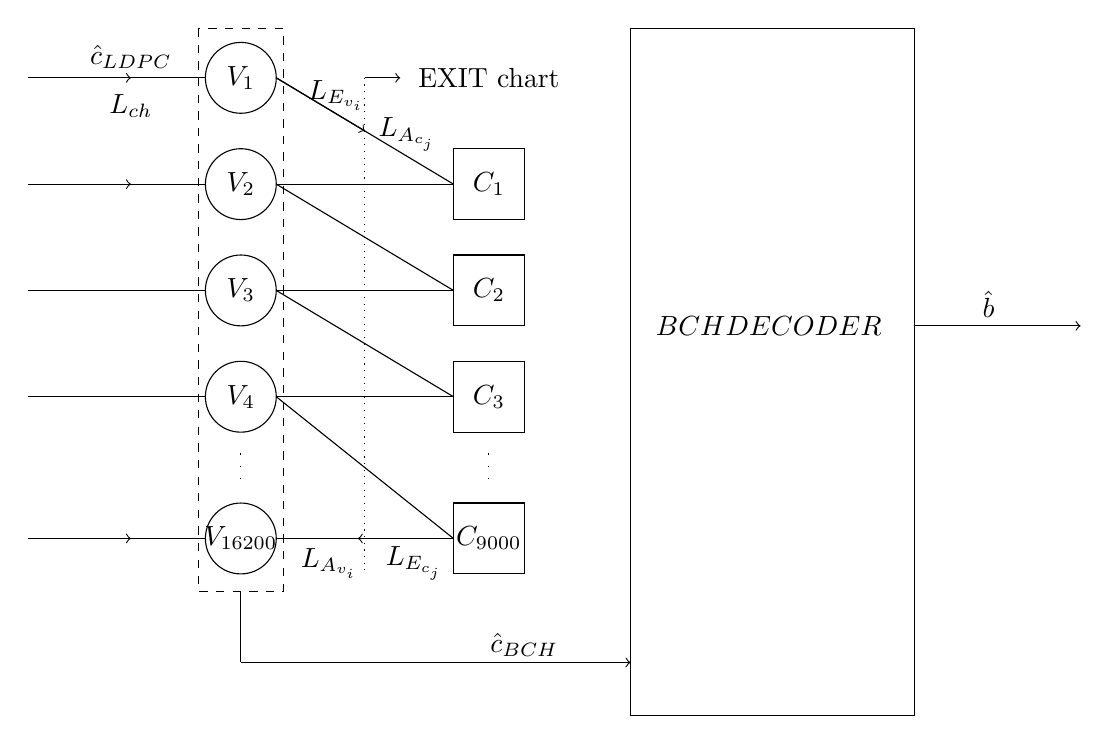
\begin{tikzpicture}[scale=0.9]
	
	\draw (1,-6) -- (2.45,-6)[->];
	\node at (2.45,-5.7) {$\hat{c}_{LDPC}$};
	\node at (2.45,-6.4) {$L_{ch}$};
	
	\draw (1,-6) -- (3.5,-6);
	\draw (1,-7.5) -- (3.5,-7.5);
	\draw (1,-7.5) -- (2.45,-7.5)[->];
	\node at (5.35,-6.25) {$L_{E_{v_{i}}}$};
	\node at (6.35,-6.8) {$L_{A_{c_{j}}}$};
	
	\draw (1,-9) -- (3.5,-9);
	\draw (1,-10.5) -- (3.5,-10.5);
	\draw (1,-12.5) -- (3.5,-12.5);
	\draw (1,-12.5) -- (2.45,-12.5)[->];
	\node at (5.25,-12.85) {$L_{A_{ v_{i}}}$};
		\node at (6.45,-12.85) {$L_{E_{c_{j}}}$};
	
	
	\draw (7,-8) rectangle (8,-7); \node at (7.5,-7.5) {$C_1$};
	\draw (7,-8.5) rectangle (8,-9.5); \node at (7.5,-9) {$C_2$};
	\draw (7,-10) rectangle (8,-11); \node at (7.5,-10.5) {$C_3$};
	\draw (7.5,-11.3) [loosely dotted]-- (7.5,-11.7);
	\draw (7,-12) rectangle (8,-13); \node at (7.5,-12.5) {$C_{9000}$};
	
	
	\draw (5.75,-6) [dotted]--  (5.75,-13);
	\draw (5.75,-6) --  (6.25,-6)[->];
	\node at (7.5,-6) {EXIT chart};
	
	
	\draw (4,-6) circle [radius=0.5]; \node at (4,-6) {$V_{1}$};
	\draw (4,-7.5) circle [radius=0.5]; \node at (4,-7.5) {$V_{2}$};
	\draw (4,-9) circle [radius=0.5]; \node at (4,-9) {$V_{3}$};
	\draw (4,-10.5) circle [radius=0.5]; \node at (4,-10.5) {$V_{4}$};
	\draw (4,-11.3) [loosely dotted] -- (4,-11.7);
	\draw (4,-12.5) circle [radius=0.5]; \node at (4,-12.5) {$V_{16200}$};
	\draw (3.4,-5.3) [dashed] rectangle (4.6,-13.25);
	\draw (4,-13.25) -- (4,-14.25);
	\draw (4,-14.25) -- (9.5,-14.25) [->];
	\draw (9.5,-5.3)  rectangle (13.5,-15); \node at (11.45,-9.5) {$BCH DECODER$};
	\draw (13.5,-9.5) -- (15.85,-9.5) [->];\node at (14.55,-9.2) {$\hat{b}$}; 
	\node at (8,-14) {$\hat{c}_{BCH}$};
	
	
	\draw (4.5,-6) -- (7,-7.5);
	\draw (4.5,-6) -- (5.75,-6.75)[->];
	
	\draw (4.5,-7.5) -- (7,-7.5);
	\draw (4.5,-7.5) -- (7,-9);
	\draw (4.5,-9) -- (7,-9);
	\draw (4.5,-9) -- (7,-10.5);
	\draw (4.5,-10.5) -- (7,-10.5);
	\draw (4.5,-10.5) -- (7,-12.5);
	\draw (4.5,-12.5) -- (7,-12.5);
	
	\draw (5.65,-12.5) -- (7,-12.5)[<-];
	
	\end{tikzpicture}
	\caption{Representasi Tanner \textit{graph} LDPC \textit{codes} DVB-T2  dengan $N_{LDPC}=16200$ dan \textit{code rate} $R_e=\frac{4}{9}$.}
\label{fig:tannerasli}
\end{figure}



\section{Usulan LDPC \textit{Codes} DVB-T2 dengan $N_{LDPC}=16200$}
LDPC \textit{codes} dibentuk menggunakan Tabel \textit{Addresses Parity Bit Accumulator} berdasarkan standar DVB-T2 untuk LDPC \textit{codes} DVB-T2 dengan panjang $N_{LDPC}=16200$. Tugas Akhir ini menyimbolkan VND $d_v$ pada LDPC \textit{codes} DVB-T2 sebagai $\Lambda (x)$, sedangkan CND $d_c$ disimbolkan sebagai $\Omega(x)$. \textit{Degree distribution} pada \textit{downscaled} LDPC \textit{codes} yang diusulkan oleh Tugas Akhir ini untuk \textit{code rate} $R_e=\frac{4}{9}$ adalah:
\begin{eqnarray}
\Lambda (x) &=& \frac{1}{16200}x+\frac{8999}{16200}x^2+\frac{5400}{16200}x^3+\frac{1800}{16200}x^8, \\
\Omega(x) &=& \frac{1441}{9000}x^4+\frac{3239}{9000}x^5+\frac{3600}{9000}x^6+\frac{720}{9000}x^7,
\end{eqnarray}
dan untuk \textit{code rate} $R_e=\frac{3}{5}$ adalah:
\begin{eqnarray}
\Lambda (x) &=& \frac{1}{16200}x+\frac{6479}{16200}x^2+\frac{6480}{16200}x^3+\frac{3240}{16200}x^{12},   \\
\Omega(x) &=& \frac{1}{6480}x^8+\frac{6479}{6480}x^9,
\end{eqnarray}
dan untuk \textit{code rate} $R_e=\frac{2}{3}$ adalah:
\begin{eqnarray}
\Lambda (x) &=& \frac{1}{16200}x+\frac{5399}{16200}x^2+\frac{9720}{16200}x^3+\frac{1080}{16200}x^{13},   \\
\Omega(x) &=& \frac{1}{5400}x^{9}+\frac{5339}{5400}x^{10},
\end{eqnarray}
dan untuk \textit{code rate} $R_e=\frac{11}{15}$ adalah:
\begin{eqnarray}
\Lambda (x) &=& \frac{1}{16200}x+\frac{4319}{16200}x^2+\frac{11520}{16200}x^3+\frac{360}{16200}x^{12},   \\
\Omega(x) &=& \frac{361}{4320}x^{9}+\frac{1079}{4320}x^{10}+\frac{1440}{4320}x^{11},+\frac{1080}{4320}x^{12}+\frac{360}{4320}x^{13},
\end{eqnarray}
dan untuk \textit{code rate} $R_e=\frac{7}{9}$ adalah:
\begin{eqnarray}
\Lambda (x) &=& \frac{1}{16200}x+\frac{3599}{16200}x^2+\frac{12600}{16200}x^3,   \\
\Omega(x) &=& \frac{361}{3600}x^{11}+\frac{1079}{3600}x^{12}+\frac{2160}{3600}x^{13},
\end{eqnarray}
dan untuk \textit{code rate} $R_e=\frac{37}{45}$ adalah:
\begin{eqnarray}
\Lambda (x) &=& \frac{1}{16200}x+\frac{2879}{16200}x^2+\frac{12960}{16200}x^3 +\frac{360}{16200}x^{13} , \\
\Omega(x) &=& \frac{1}{2880}x^{15}+\frac{1439}{2880}x^{16}+\frac{360}{2880}x^{17}+\frac{360}{2880}x^{18}+\frac{720}{2880}x^{19}.
\end{eqnarray}
\section{Usulan LDPC \textit{Codes} DVB-T2 menggunakan Teknik \textit{Downscaling}}

Teknik \textit{downscaling} digunakan untuk mengurangi kompleksitas komputasi pada \textit{encoder} dan \textit{decoder}, sehingga akan meringankan proses simulasi dan memungkinkan untuk \textit{device} dengan kemampuan komputasi rendah \cite{scale}. Langkah-langkah untuk melakukan \textit{downscaling} LDPC \textit{codes} DVB-T2 adalah sebagai berikut: 

\begin{enumerate}
	\item Tentukan \textit{scaling factor} $s_f$, $s_f$ harus merupakan faktor dari $360$. 
	\item Masukkan nilai pada Tabel \textit{Addresses Parity Bit Accumulator} seperti pada Tabel \ref{table:adressldpc} ke $p_{1}(j), p_{2}(j), p_{3}(j), \dots$$, p_{q}(j)$, $j= 1, 2, 3, \dots, J$  dan $q= 1, 2, 3, \dots, Q$. 
%	$j$ menunjukkan kolom dan  $q$ menunjukkan baris dari Tabel \ref{table:dvb-t2lite}.
	\item Hitung $r_{1}(j), r_{2}(j), r_{3}(j), \dots, r_{q}(j)$
	\begin{equation}
	r_{q}(j)=mod\left \{ \left [ p_q(j) + J \times \left ( k-1 \right ) \right ],\left [ P/s_f \right ] \right \},
	\end{equation}
	\item Nilai $r_q(j)$ akan menjadi Tabel \textit{Addresses Parity Bit Accumulator} baru untuk \textit{downscaled} LDPC \textit{codes} DVB-T2. 
\end{enumerate}
Parameter $q$ adalah kolom dan $j$ adalah baris dari Tabel \textit{Addresses Parity Bit Accumulators}.  Nilai $s_f$ akan menentukan panjang blok matriks \textit{parity check} \textit{downscaled} LDPC \textit{codes} DVB-T2. $P$ adalah nilai dari baris original matriks LDPC \textit{codes} DVB-T2, nilai $k$ memiliki batas dengan $1< k \leq \left ( 360/s_f \right )$. Nilai $360$ adalah jumlah \textit{node indices} LDPC \textit{codes} DVB-T2.


\begin{figure}[b!]
	\centering
	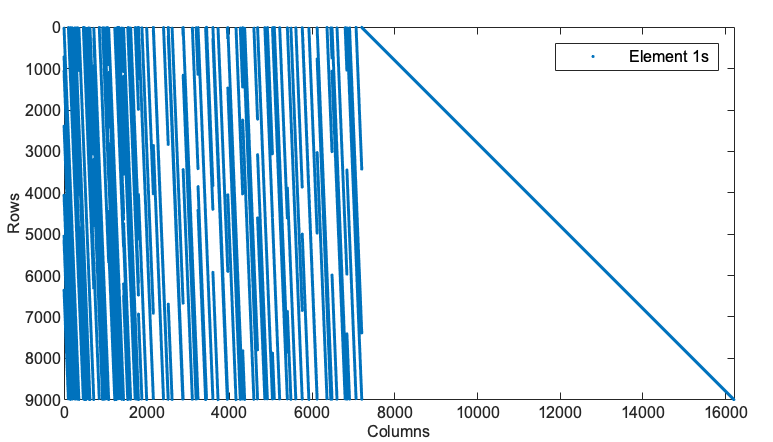
\includegraphics[width=1\textwidth]
	{pics/hs(1-2)-2}
	\caption{Matriks \textit{parity check} original DVB-T2 LDPC \textit{codes} dengan $N_{LDPC}=16200$.}
	\label{fig:hori}
\end{figure}

%\begin{figure}
%	\centering
%%	\hspace{-0.2 in}
%	\begin{minipage}{1\linewidth}
%		\hspace{1.5 cm}
%		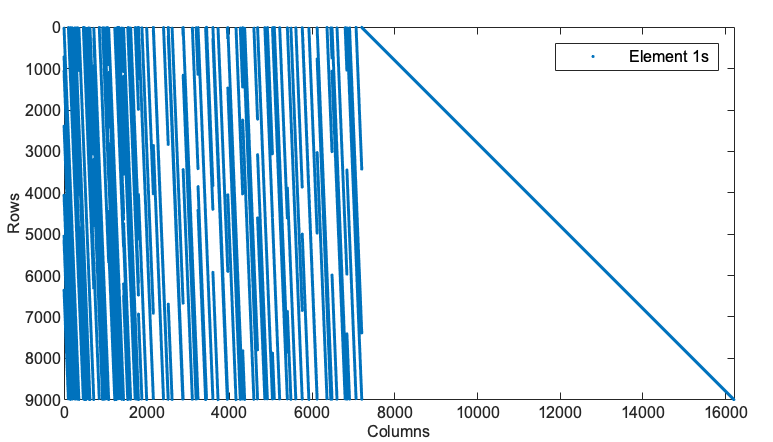
\includegraphics[width=0.9\textwidth]{pics/hs(1-2)-2}
%		\vspace{-0.5cm}
%		
%		\center (a)
%	\end{minipage}
%	\hfill
%%	\hspace{0.05 in}
%	\begin{minipage}{1\linewidth}
%		\hspace{1.5 cm}
%		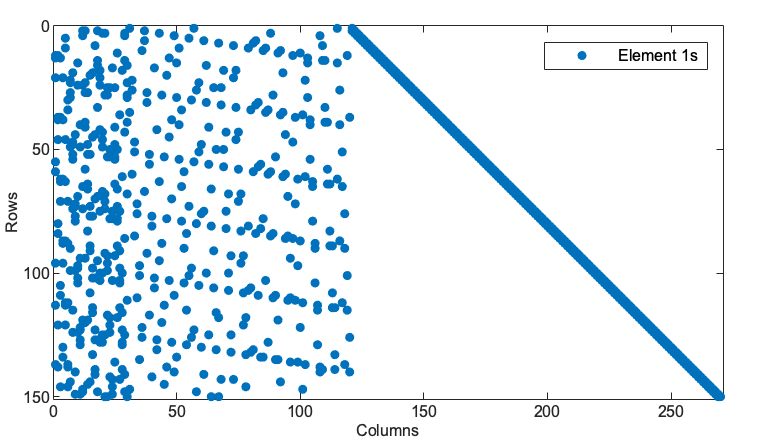
\includegraphics[width=0.9\textwidth]{pics/hs1-60(1-2)-2}
%		\vspace{-0.5cm}
%		\center (b)
%	\end{minipage}
%	\caption {Matriks \textit{parity check} DVB-T2 LDPC \textit{codes} (a) $N_{LDPC}=16200$ dan (b) $N_{LDPC}=270$.}
%	\label{gambar: banding}
%\end{figure}


\begin{figure}[t!]
	\centering
	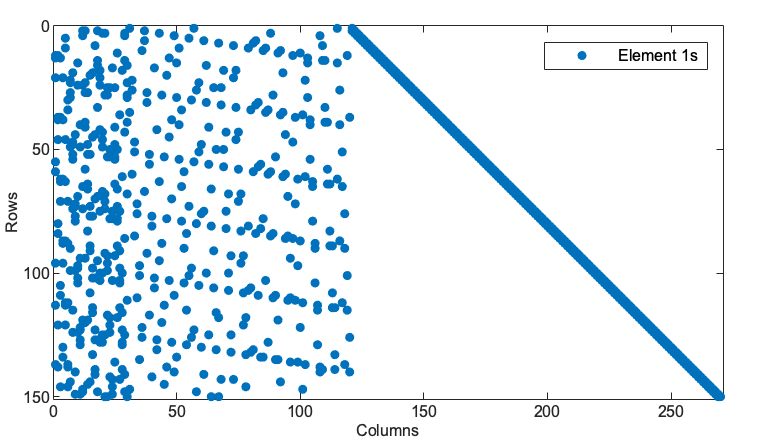
\includegraphics[width=1\textwidth]
	{pics/hs1-60(1-2)-2}
	\caption{Matriks \textit{downscaled} \textit{parity check} DVB-T2 LDPC \textit{codes} dengan $N_{LDPC}=270$.}
	\label{fig:hds}
\end{figure}
%\begin{figure}[tb]
%	\centering 
%
%	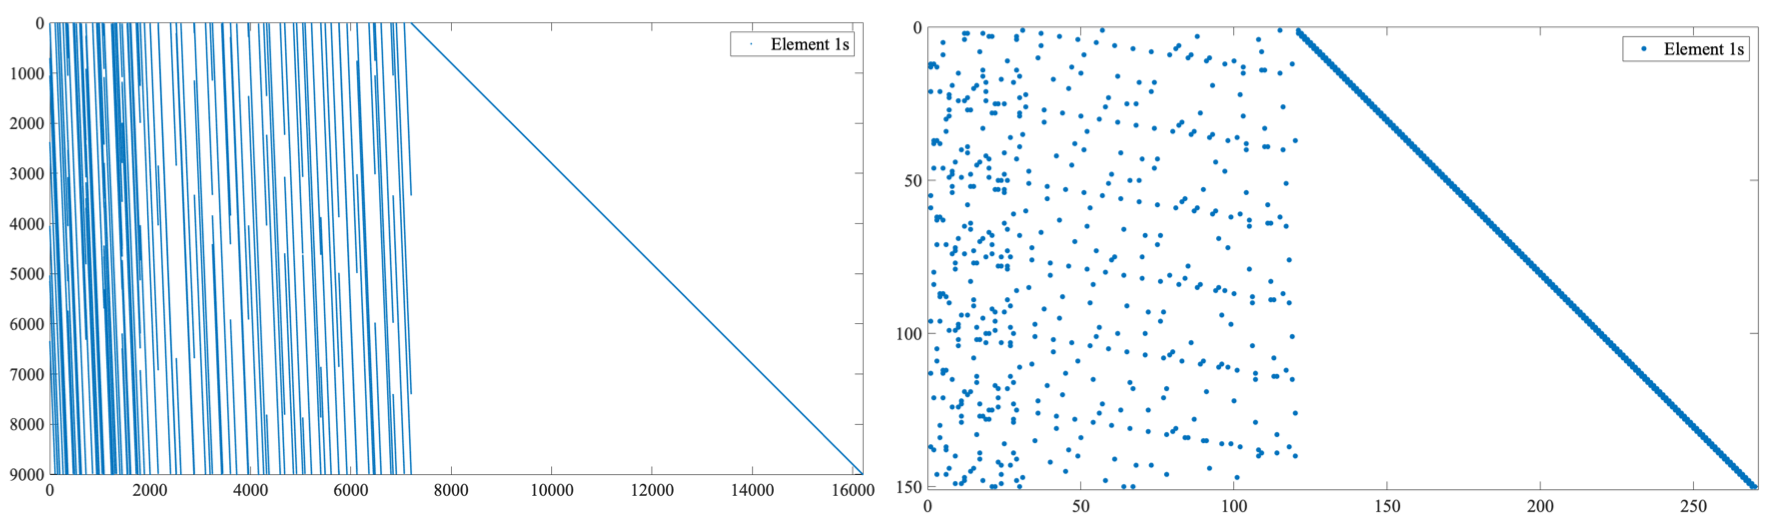
\includegraphics[scale=0.5]{pics/banding}
%	\centering 
%	\caption{Perbandingan matriks \textit{parity check} LDPC \textit{codes} DVB-T2 original dengan \textit{downscaled}.}
%	\label{fig:banding}
%\end{figure}

Tugas Akhir ini menggunakan \textit{scaling factor} $s_f=60$ untuk mengetahui efek \textit{downscaling} pada kinerja LDPC \textit{codes} DVB-T2  dan meringankan proses simulasi. \textit{Downscaled} matriks \textit{parity check}  LDPC \textit{codes} ditunjukkan oleh Gambar  \ref{fig:hds}, sedangkan original matriks \textit{parity check}  LDPC \textit{codes} ditunjukkan oleh Gambar \ref{fig:hori}. Tugas Akhir ini telah melakukan \textit{downscaling} untuk semua \textit{code rate} pada LDPC \textit{codes} DVB-T2, karena $s_f=60$ maka \textit{downscaled} LDPC \textit{codes} DVB-T2 memiliki panjang blok $N_{LDPC}=270$.

Tugas Akhir ini menyimbolkan VND $d_v$ pada LDPC \textit{codes} DVB-T2 sebagai $\Lambda (x)$, sedangkan CND $d_c$ disimbolkan sebagai $\Omega(x)$. \textit{Degree distribution} pada \textit{downscaled} LDPC \textit{codes} yang diusulkan oleh Tugas Akhir ini untuk \textit{code rate} $R_e=\frac{4}{9}$ adalah:
\begin{eqnarray}
\Lambda (x)&=&\frac{1}{270}x+\frac{149}{270}x^2+\frac{90}{270}x^3+\frac{30}{270}x^8, \\
\Omega(x)&=&\frac{25}{150}x^4+\frac{53}{150}x^5+\frac{60}{150}x^6+\frac{12}{150}x^{12},
\end{eqnarray}
untuk \textit{code rate} $R_e=\frac{3}{5}$ adalah:
\begin{eqnarray}
\Lambda (x)&=&\frac{1}{270}x+\frac{107}{270}x^2+\frac{132}{270}x^3+\frac{30}{270}x^{12},\\
\Omega(x)&=&\frac{1}{108}x^8+\frac{107}{108}x^9,
\end{eqnarray}
untuk \textit{code rate} $R_e=\frac{2}{3}$ adalah:
\begin{eqnarray}
\Lambda (x)&=&\frac{1}{270}x+\frac{89}{270}x^{2}+\frac{162}{270}x^{3}+\frac{18}{270}x^{13},\\
\Omega(x)&=&\frac{1}{90}x^{9}+\frac{89}{90}x^{10},
\end{eqnarray}
untuk \textit{code rate} $R_e=\frac{11}{15}$ adalah:
\begin{eqnarray}
\Lambda (x)&=&\frac{1}{270}x+\frac{71}{270}x^{2}+\frac{192}{270}x^{3}+\frac{6}{270}x^{12},\\
\Omega(x)&=&\frac{7}{72}x^{9}+\frac{11}{72}x^{10}+\frac{36}{72}x^{11}+\frac{12}{72}x^{12} \nonumber \\ &&+\frac{6}{72}x^{13}.
\end{eqnarray}
untuk \textit{code rate} $R_e=\frac{7}{9}$ adalah:
\begin{eqnarray}
\Lambda (x)&=&\frac{1}{270}x+\frac{71}{270}x^2+\frac{198}{270}x^3,\\
\Omega(x)&=&\frac{7}{60}x^{11}+\frac{29}{60}x^{12}+\frac{24}{60}x^{13},
\end{eqnarray}
dan untuk \textit{code rate} $R_e=\frac{37}{45}$ adalah:
\begin{eqnarray}
\Lambda (x)&=&\frac{1}{270}x+\frac{71}{270}x^{2}+\frac{192}{270}x^{3}+\frac{6}{270}x^{12},\\
\Omega(x)&=&\frac{7}{48}x^{15}+\frac{17}{48}x^{16}+\frac{18}{48}x^{17}+\frac{6}{48}x^{18},
\end{eqnarray}
\textit{Degree distribution} untuk setiap \textit{code rate} tetap memenuhi ketentuan pada Tabel \ref{table:dvb-t2lite} dengan jumlah yang disesuaikan pada ukuran matriksnya.

\section{Usulan Algoritma PEG}
Tugas Akhir ini mengusulkan Algoritma PEG menggunakan metode kedua dari PEG yaitu dengan memilih nilai CND terkecil secara terurut. Pada langkah kedua PEG, Tugas Akhir ini menambahkan sebuah algoritma untuk menghindari pembentukkan LDPC \textit{codes} dengan \textit{girth}-4 yang dinamakan algoritma \textit{Anti Girth}-4. Penggunaan PEG dalam pembuatan matriks \textit{parity check} LDPC \textit{codes} memungkinkan untuk membuat matriks \textit{parity check} LDPC \textit{codes} sesuai dengan nilai panjang blok $n$, baris $m$, dan set dari VND~$D_v=\{ d_{v_1}, d_{v_2}, d_{v_3}, \cdots ,d_{v_n} \}$ yang telah ditentukan. Proses penempatan elemen 1 dimulai dari kolom 1 sampai $n$ dan dari baris 1 ke $m$ yang prosesnya berjalan dari kiri ke kanan dan dari atas ke bawah.

\subsection{Langkah PEG}
Langkah-langkah perancangan matriks \textit{parity check} LDPC \textit{codes} menggunakan algoritma PEG yang diusulkan dengan nilai $n=8$, $m=5$, dan $D_v=\{ 2, 2, 2, 2 ,2 \}$ adalah sebagai berikut:
%\begin{equation}
%%\begin{figure}
%%	\centering 
%%		\hspace{0.75cm}
%%	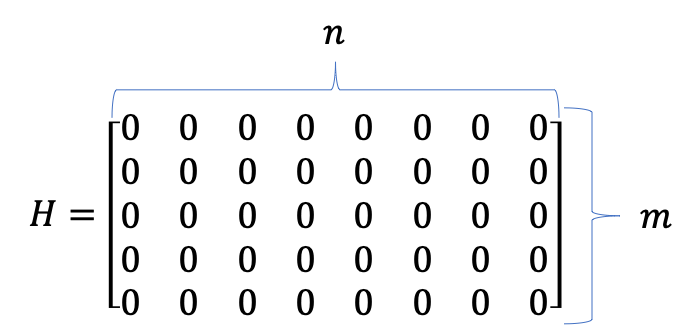
\includegraphics[scale=0.5]{pics/step1}
%%	\centering 
%\mathbf{B}_r=
%\begin{tikzpicture}[baseline=-\the\dimexpr\fontdimen22\textfont2\relax ]
%\matrix (m)[matrix of math nodes,left delimiter=(,right delimiter=)]
%{
%	0 & 0 & 1 & 0 \\
%	1 & 0 & 1 & 0 \\
%	1 & 0 & 1 & 1 \\
%	0 & 1 & 0 & 1 \\
%};
%\begin{pgfonlayer}{myback}
%\fhighlight[green!30]{m-1-3}{m-4-3}
%\end{pgfonlayer}
%\end{tikzpicture}
%
%%\end{figure}
%\end{equation}


\begin{equation}
\mathbf{H}=
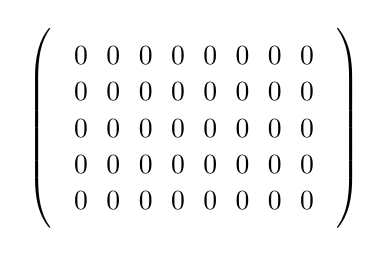
\begin{tikzpicture}[baseline=-\the\dimexpr\fontdimen22\textfont2\relax ]
\matrix (m)[matrix of math nodes,left delimiter=(,right delimiter=)]
{
	0 & 0 & 0 & 0 & 0 & 0 & 0 & 0\\
	0 & 0 & 0 & 0 & 0 & 0 & 0 & 0\\
	0 & 0 & 0 & 0 & 0 & 0 & 0 & 0\\
	0 & 0 & 0 & 0 & 0 & 0 & 0 & 0\\
	0 & 0 & 0 & 0 & 0 & 0 & 0 & 0 \\
};
\begin{pgfonlayer}{myback}
%\fhighlight[green!30]{m-1-3}{m-4-3}
\end{pgfonlayer}
\end{tikzpicture}
\end{equation}

\begin{itemize}
	\item[1.] Buat matriks nol dengan dimensi $m\times n$, dengan $n$ adalah jumlah variable \textit{nodes} dan $m$ adalah jumlah \textit{check nodes} yang telah ditentukan.
\end{itemize}
%\begin{figure}
%	\centering 
%	
\includegraphics[scale=0.5]{pics/step2}
%	\centering 
%\end{figure}
\begin{equation}
\mathbf{H}=
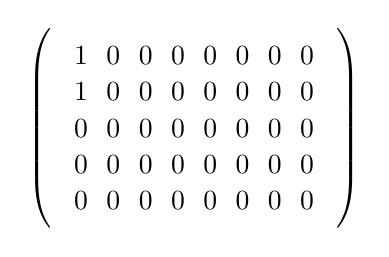
\begin{tikzpicture}[baseline=-\the\dimexpr\fontdimen22\textfont2\relax ]
\matrix (m)[matrix of math nodes,left delimiter=(,right delimiter=)]
{
	1 & 0 & 0 & 0 & 0 & 0 & 0 & 0\\
	1 & 0 & 0 & 0 & 0 & 0 & 0 & 0\\
	0 & 0 & 0 & 0 & 0 & 0 & 0 & 0\\
	0 & 0 & 0 & 0 & 0 & 0 & 0 & 0\\
	0 & 0 & 0 & 0 & 0 & 0 & 0 & 0 \\
};
\begin{pgfonlayer}{myback}
%\fhighlight[green!30]{m-1-3}{m-4-3}
\end{pgfonlayer}
\end{tikzpicture}
\end{equation}
\begin{itemize}
	\item[2.] Elemen 1 pertama ditempatkan sesuai dengan algoritma pertama dari proses PEG. Elemen 1 kedua dan seterusnya sebanyak $d_v(n)$ ditempatkan menggunakan kombinasi algoritma PEG dengan \textit{Anti Girth}-4.
\end{itemize}
%\begin{figure}
%	\centering 
%	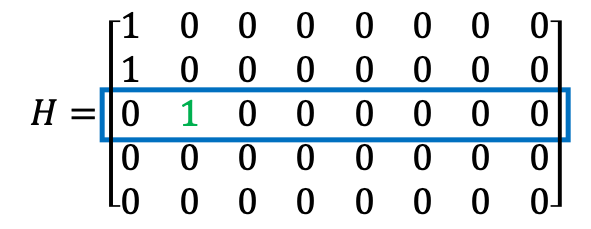
\includegraphics[scale=0.5]{pics/step3}
%	\centering 
%\end{figure}
\begin{equation}
\mathbf{H}=
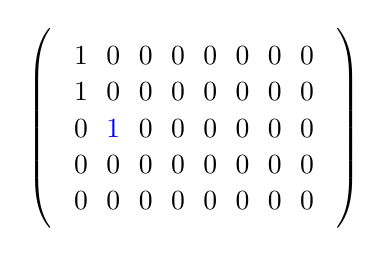
\begin{tikzpicture}[baseline=-\the\dimexpr\fontdimen22\textfont2\relax ]
\matrix (m)[matrix of math nodes,left delimiter=(,right delimiter=)]
{
	1 & 0 & 0 & 0 & 0 & 0 & 0 & 0\\
	1 & 0 & 0 & 0 & 0 & 0 & 0 & 0\\
	0 & \color{blue}1 & 0 & 0 & 0 & 0 & 0 & 0\\
	0 & 0 & 0 & 0 & 0 & 0 & 0 & 0\\
	0 & 0 & 0 & 0 & 0 & 0 & 0 & 0 \\
};
\begin{pgfonlayer}{myback}
\fhighlight[green!30]{m-3-1}{m-3-8}
\end{pgfonlayer}
\end{tikzpicture}
\end{equation}
\begin{itemize}
	\item[3.] Elemen 1 ditempatkan pada \textit{check node} urutan pertama dengan nilai CND terendah.
\end{itemize}

%\begin{figure}
%	\centering 
%	
\includegraphics[scale=0.5]{pics/step4}
%	\centering 
%\end{figure}

\begin{equation}
\mathbf{H}=
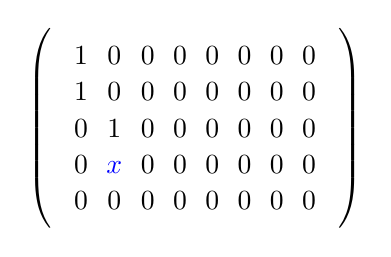
\begin{tikzpicture}[baseline=-\the\dimexpr\fontdimen22\textfont2\relax ]
\matrix (m)[matrix of math nodes,left delimiter=(,right delimiter=)]
{
	1 & 0 & 0 & 0 & 0 & 0 & 0 & 0\\
	1 & 0 & 0 & 0 & 0 & 0 & 0 & 0\\
	0 & 1 & 0 & 0 & 0 & 0 & 0 & 0\\
	0 & \color{blue}x & 0 & 0 & 0 & 0 & 0 & 0\\
	0 & 0 & 0 & 0 & 0 & 0 & 0 & 0 \\
};
\begin{pgfonlayer}{myback}
%\fhighlight[green!30]{m-3-1}{m-3-8}
\end{pgfonlayer}
\end{tikzpicture}
\end{equation}

\begin{itemize}
	\item[4.] Simbol $x$ adalah calon letak elemen 1, $x$ dipilih berdasarkan baris yang memiliki nilai CND terendah. Kemudian langkah berikutnya menggunakan algoritma \textit{Anti Girth}-4, melakukan pengeceken ke kiri apabila tidak ada elemen satu maka letak tersebut akan menjadi elemen 1.
\end{itemize}

%\begin{figure}
%	\centering 
%	\hspace{1.6cm}
%	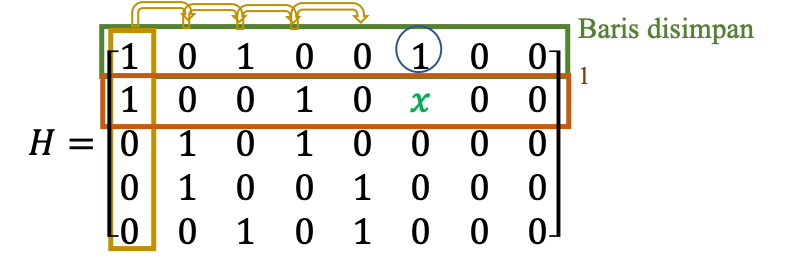
\includegraphics[scale=0.5]{pics/step5}
%	\centering 
%\end{figure}

\begin{equation}
\mathbf{H}=
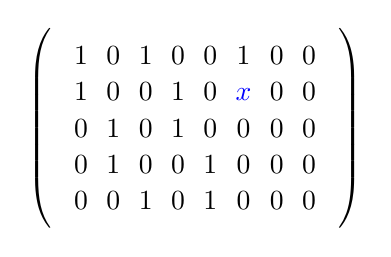
\begin{tikzpicture}[baseline=-\the\dimexpr\fontdimen22\textfont2\relax ]
\matrix (m)[matrix of math nodes,left delimiter=(,right delimiter=)]
{
	1 & 0 & 1 & 0 & 0 & 1 & 0 & 0\\
	1 & 0 & 0 & 1 & 0 & \color{blue}x & 0 & 0\\
	0 & 1 & 0 & 1 & 0 & 0 & 0 & 0\\
	0 & 1 & 0 & 0 & 1 & 0 & 0 & 0\\
	0 & 0 & 1 & 0 & 1 & 0 & 0 & 0 \\
};
\begin{pgfonlayer}{myback}
\fhighlight[green!30]{m-2-1}{m-2-8}
\fhighlight[red!30]{m-1-1}{m-5-1}
\fhighlight[yellow!30]{m-1-6}{m-1-6}
\end{pgfonlayer}
\end{tikzpicture}
\end{equation}

\begin{itemize}
	\item[5.] Algoritma \textit{Anti Girth}-4 dimulai dengan menyimpan, baris dari elemen 1 sebelumnya yang nantinya akan digunakan pada pengecekan akhir. Kemudian melakukan pengecekan dari kiri ke kanan apabila ditemukan elemen 1, maka akan berlanjut ke langkah berikutnya. Apabila tidak ditemukan elemen 1 pada kolom tersebut, maka $x$ akan menjadi elemen 1. Pengecekan akan dilakukan sampai kolom sebelum kolom $x$.
\end{itemize}

%\begin{figure}
%	\centering 
%	\hspace{-1.2cm}
%	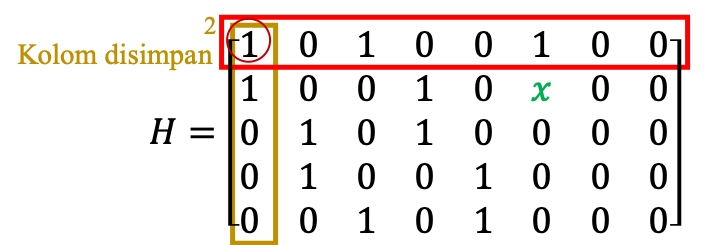
\includegraphics[scale=0.5]{pics/step6}
%	\centering 
%\end{figure}

\begin{equation}
\mathbf{H}=
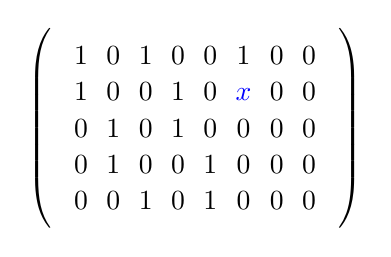
\begin{tikzpicture}[baseline=-\the\dimexpr\fontdimen22\textfont2\relax ]
\matrix (m)[matrix of math nodes,left delimiter=(,right delimiter=)]
{
	1 & 0 & 1 & 0 & 0 & 1 & 0 & 0\\
	1 & 0 & 0 & 1 & 0 & \color{blue}x & 0 & 0\\
	0 & 1 & 0 & 1 & 0 & 0 & 0 & 0\\
	0 & 1 & 0 & 0 & 1 & 0 & 0 & 0\\
	0 & 0 & 1 & 0 & 1 & 0 & 0 & 0 \\
};
\begin{pgfonlayer}{myback}
\fhighlight[green!30]{m-1-1}{m-1-8}
\fhighlight[red!30]{m-1-1}{m-5-1}
\fhighlight[yellow!30]{m-1-1}{m-1-1}
\end{pgfonlayer}
\end{tikzpicture}
\end{equation}

\begin{itemize}
	\item[6.] Langkah ke-2 Algoritma \textit{Anti Girth}-4, menyimpan kolom dari elemen 1 yang ditemukan pada proses pengecekan di langkah pertama. 
	\item [7.] Kemudian melakukan pengecekan akhir, yaitu apabila
	\begin{equation}
	\mathbf{H}_{Baris\_simpan, Kolom\_simpan}=1,
	\end{equation}
	pada $x$ akan terbentuk \textit{girth} 4 jika $x$ berelemen 1, sehingga $x$ akan berpindah ke \textit{check node} dengan CND minimal berikutnya dan melakukan pengecekan lagi.
\end{itemize}

Matriks \textit{parity check} LDPC \textit{codes} yang terbentuk dan graf pohon pada variable \textit{nodes} ke-dua menggunakan aturan PEG ditunjukkan oleh Gambar \ref{fig:PEGM}. Dapat diketahui bahwa matriks \textit{parity check} tidak menghasilkan \textit{girth}-4.
\begin{figure}[tb]
	\centering 
	\hspace{-1.2cm}
	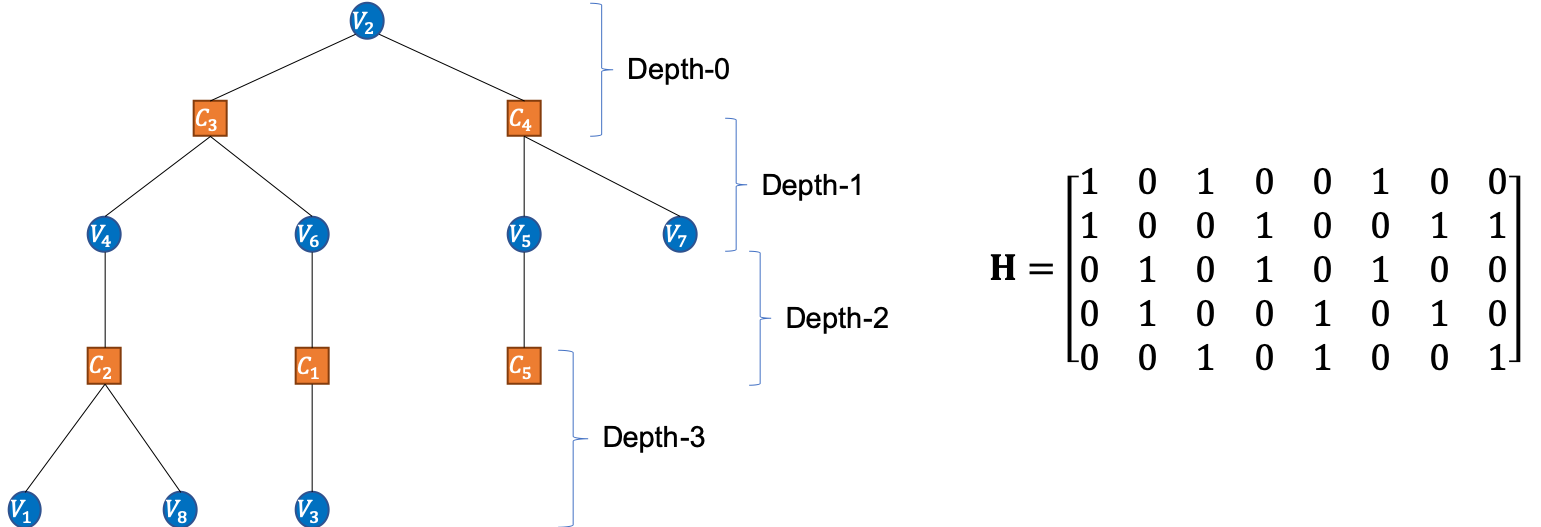
\includegraphics[width=1\textwidth]{pics/withmatlabpeg2}
	\centering 
	\caption{Hasil graf pohon dan matriks \textit{parity check} LDPC \textit{codes} menggunakan algoritma PEG yang diusulkan.}
	\label{fig:PEGM}
\end{figure}

\subsection{Usulan LDPC \textit{Codes} DVB-T2 menggunakan PEG}
Tugas Akhir ini juga mengusulkan \textit{degree distribution} untuk \textit{downscaled} LDPC \textit{codes} DVB-T2 dengan menggunakan algoritma PEG. \textit{Degree distribution} pada \textit{downscaled} LDPC \textit{codes} yang diusulkan untuk \textit{code rate} $R_e=\frac{4}{9}$ adalah:
\begin{eqnarray}
\Lambda (x) &=& \frac{1}{270}x+\frac{149}{270}x^2+\frac{90}{270}x^3+\frac{30}{270}x^8 \\
\Omega(x) &=& \frac{92}{150}x^5+\frac{58}{150}x^6,
\end{eqnarray}
untuk \textit{code rate} $R_e=\frac{3}{5}$ adalah:
\begin{eqnarray}
\Lambda (x) &=& \frac{1}{270}x+\frac{107}{270}x^2+\frac{132}{270}x^3+\frac{1}{270}x^7+\frac{7}{270}x^8 \nonumber \\ &&+\frac{1}{270}x^9+\frac{11}{270}x^{10}+\frac{10}{270}x^{12},   \\
\Omega(x) &=& \frac{59}{108}x^8+\frac{49}{108}x^9,
\end{eqnarray}
untuk \textit{code rate} $R_e=\frac{2}{3}$ adalah:
\begin{eqnarray}
\Lambda (x) &=& \frac{1}{270}x+\frac{89}{270}x^2+\frac{162}{270}x^3+\frac{1}{270}x^7 \nonumber \\ &&+\frac{9}{270}x^8+\frac{1}{270}x^{12}+\frac{7}{270}x^{13} ,  \\
\Omega(x) &=& \frac{37}{90}x^{10}+\frac{53}{90}x^9,
\end{eqnarray}
untuk \textit{code rate} $R_e=\frac{11}{15}$ adalah:
\begin{eqnarray}
\Lambda (x) &=& \frac{1}{270}x+\frac{71}{270}x^2+\frac{192}{270}x^3+\frac{6}{270}x^{12},   \\
\Omega(x) &=& \frac{4}{72}x^{10}+\frac{65}{72}x^{11},+\frac{3}{72}x^{12},
\end{eqnarray}
untuk \textit{code rate} $R_e=\frac{7}{9}$ adalah:
\begin{eqnarray}
\Lambda (x) &=& \frac{1}{270}x+\frac{59}{270}x^2+\frac{210}{270}x^3,  \\
\Omega(x) &=& \frac{31}{60}x^{12}+\frac{29}{60}x^{13},
\end{eqnarray}
untuk \textit{code rate} $R_e=\frac{37}{45}$ adalah:
\begin{eqnarray}
\Lambda (x) &=& \frac{1}{270}x+\frac{76}{270}x^2+\frac{185}{270}x^3 +\frac{2}{270}x^4+\frac{1}{270}x^{12}+\frac{3}{270}x^{13},  \\
\Omega(x) &=& \frac{5}{48}x^{15}+\frac{39}{48}x^{16}+\frac{2}{48}x^{17}+\frac{2}{48}x^{18}.
\end{eqnarray}


%\subsection{\textit{Formatting} Tulisan}
%\begin{itemize}
%\item Tulisan Tebal (\textit{Bold})\\
%\textbackslash textbf\{\textit{argument}\} untuk menebalkan tulisan.\\
%contoh:
%\textbackslash textbf\{tulisan tebal\} $\rightarrow$ \textbf{tulisan tebal}
%
%\item Tulisan Miring (\textit{Italic})\\
%\textbackslash textit\{\textit{argument}\} untuk memiringkan tulisan.\\
%contoh:
%\textbackslash textit\{tulisan miring\} $\rightarrow$ \textit{tulisan miring}
%
%\item Tulisan Bergaris Bawah (\textit{Underlined})\\
%\textbackslash uline\{\textit{argument}\} untuk menggarisbahwahi tulisan.\\
%contoh:
%\textbackslash uline\{tulisan bergaris bawah\} $\rightarrow$ \uline{tulisan bergaris bawah}
%
%\item Tulisan Menggantung ke Atas (\textit{Superscript})\\
%\textbackslash textsuperscript\{\textit{argument}\} untuk membuat tulisan menggantung.\\
%contoh:
%\textbackslash textsuperscript\{tulisan menggantung\} $\rightarrow$ \textsuperscript{tulisan menggantung ke atas}
%
%\item Tulisan Menggantung ke Bawah (\textit{Subscript})\\
%\textbackslash textsubscript\{\textit{argument}\} untuk membuat tulisan menggantung.\\
%contoh:
%\textbackslash textsubscript\{tulisan menggantung\} $\rightarrow$ \textsubscript{tulisan menggantung ke bawah}
%
%\item Tulisan yang Dicoret (\textit{Strike-through})
%\textbackslash sout\{\textit{argument}\} untuk membuat tulisan tercoret.\\
%contoh:
%\textbackslash sout\{tulisan tercoret\} $\rightarrow$ \sout{tulisan tercoret}
%\end{itemize}
%
%\subsection{Memasukkan Gambar}
%Untuk memasukkan gambar ke dalam dokumen, digunakan \textit{syntax} \textbackslash begin\{figure\} ... \textbackslash end\{figure\}. Berikut contoh memasukkan \textit{file} gambar \textit{bipartite.png} yang berada di dalam folder \textit{pics/diagram/}. Dari kode tersebut didapatkan hasil gambar \ref{fig:bipartite}. Label dapat diberikan di dalam \textit{figure}, sehingga untuk merujuk sebuah gambar dapat digunakan \textit{ref}. Contoh penggunaan \textit{ref}, misalkan \textbackslash ref\{fig:bipartite\} $\rightarrow$ \ref{fig:bipartite}.
%
%\begin{lstlisting}
%\begin{figure}
%	\centering
%	\includegraphics[width=0.6\textwidth]
%		{pics/diagram/bipartite.png}
%		\caption{Topologi \textit{Bipartite} untuk Pengukuran Fail-Over Delay}
%	\label{fig:bipartite}
%\end{figure}
%\end{lstlisting}
%
%\begin{figure}
%	\centering
%	\includegraphics[width=0.6\textwidth]
%		{pics/diagram/bipartite.png}
%		\caption{Topologi \textit{Bipartite} untuk Pengukuran Fail-Over Delay}
%	\label{fig:bipartite}
%\end{figure}
%
%\subsection{Membuat Tabel}
%Untuk memasukkan tabel ke dalam dokumen, digunakan \textit{syntax} \textbackslash begin\{table\} ... \textbackslash end\{table\}
%
%\begin{lstlisting}
%\begin{table}
%	\centering
%	\caption{Jumlah \textit{Switch} dan \textit{Host} serta Jenis \textit{Traffic} untuk Setiap Pengukuran}
%	\label{tab:tab1}
%	\begin{tabular}{| l | r | r | r | c |}
%		\hline
%		Pengukuran & L1 & L2 & \textit{Host} & \textit{Traffic}\\ 
%		\hline
%		\textit{Fail-Over Delay} & 2 - 4  & 1 - 8 & 1 - 8 & ICMP Ping Tunggal\\
%		\textit{Load Balance: Load Distribution} & 1 - 4 & 1 & 1 & 200 UDP \textit{Flows}\\
%		\textit{Load Balance: Performance} & 1 - 4  & 1 - 8 & 1 - 8 & Data, Video, VoIP \textit{Flows}\\
%		\textit{Overhead Size} & 2 & 1 & 1 & 25 - 150 UDP \textit{Flows}\\
%		\textit{Memory Consumption: Switch} & 1 - 4  & 1 - 8 & 0 & -\\
%		\textit{Memory Consumption: Host}  & 1 & 1 & 0 - 200 & - \\
%		\hline
%	\end{tabular}
%\end{table}
%\end{lstlisting}
%
%\begin{table}
%	\centering
%	\caption{Jumlah \textit{Switch} dan \textit{Host} serta Jenis \textit{Traffic} untuk Setiap Pengukuran}
%	\label{tab:tab1}
%	\begin{tabular}{| l | r | r | r | c |}
%		\hline
%		Pengukuran & L1 & L2 & \textit{Host} & \textit{Traffic}\\ 
%		\hline
%		\textit{Fail-Over Delay} & 2 - 4  & 1 - 8 & 1 - 8 & ICMP Ping Tunggal\\
%		\textit{Load Balance: Load Distribution} & 1 - 4 & 1 & 1 & 200 UDP \textit{Flows}\\
%		\textit{Load Balance: Performance} & 1 - 4  & 1 - 8 & 1 - 8 & Data, Video, VoIP \textit{Flows}\\
%		\textit{Overhead Size} & 2 & 1 & 1 & 25 - 150 UDP \textit{Flows}\\
%		\textit{Memory Consumption: Switch} & 1 - 4  & 1 - 8 & 0 & -\\
%		\textit{Memory Consumption: Host}  & 1 & 1 & 0 - 200 & - \\
%		\hline
%	\end{tabular}
%\end{table}
%
%\subsection{Notasi Matematika}
%Untuk menuliskan notasi matematika, pada \latex digunakan \textit{syntax} \$ ... \$ untuk penggunaan di dalam paragraf dan \textbackslash begin\{equation\} ... \textbackslash end\{equation\} untuk penggunaan terpisah di luar paragraf. Sebagai contoh sebagai berikut.
%\begin{itemize}
%\item contoh 1:
%\begin{lstlisting}
%\begin{equation}
%	metric_{i,j} = \frac{10^2}{(capacity_{E_{i,j}} - 	load_{E_{i,j}})}
%	\label{eq:metric1}
%\end{equation}
%\end{lstlisting}
%\begin{equation}
%	metric_{i,j} = \frac{10^2}{(capacity_{E_{i,j}} - 	load_{E_{i,j}})}
%	\label{eq:metric1}
%\end{equation}
%\item contoh 2:
%\begin{lstlisting}
%\begin{equation}
%	f(x)=(x+a)(x+b)
%	\label{eq:fx1}
%\end{equation}
%\end{lstlisting}
%\begin{equation}
%	f(x)=(x+a)(x+b)
%	\label{eq:fx1}
%\end{equation}
%\item contoh 3
%\begin{lstlisting}
%\begin{subequations}
%Maxwell's equations:
%	\begin{align}
%		B'&=-\nabla \times E,\\
%		E'&=\nabla \times B - 4\pi j,
%	\end{align}
%	\label{eq:maxwell}
%\end{subequations}
%\end{lstlisting}
%\begin{subequations}
%Maxwell's equations:
%	\begin{align}
%		B'&=-\nabla \times E,\\
%		E'&=\nabla \times B - 4\pi j,
%	\end{align}
%	\label{eq:maxwell}
%\end{subequations}
%\item contoh 4
%\begin{lstlisting}[language=tex]
%matriks $Adj$ digunakan untuk menggambarkan topologi jaringan  $G = (V,E)$, di mana $V = \{v_{1}, v_{2}, ..., v_{n}\}$ merupakan \textit{switch} dan $E = \{e_{1,1}, e_{1,2}, ..., e_{n,n}\}$ merupakan \textit{link} antar-\textit{switch}. Setiap $E_{i,j}$ menyimpan informasi \textit{metric} sesuai persamaan \ref{eq:metric1} . Hasil dari algoritma ini adalah jalur $T_{k,l}$ yang disimpan di dalam \textit{bucket Path} atau $T$. Setiap $T_{k,l}$ mempunyai nilai \textit{metric} sesuai persamaan \ref{eq:metric2}.
%\end{lstlisting}
%matriks $Adj$ digunakan untuk menggambarkan topologi jaringan  $G = (V,E)$, di mana $V = \{v_{1}, v_{2}, ..., v_{n}\}$ merupakan \textit{switch} dan $E = \{e_{1,1}, e_{1,2}, ..., e_{n,n}\}$ merupakan \textit{link} antar-\textit{switch}. Setiap $E_{i,j}$ menyimpan informasi \textit{metric} sesuai persamaan \ref{eq:metric1}. Hasil dari algoritma ini adalah jalur $T_{k,l}$ yang disimpan di dalam \textit{bucket Path} atau $T$. Setiap $T_{k,l}$ mempunyai nilai \textit{metric} sesuai persamaan 3.2.
%\end{itemize} 
%
%\subsection{Notasi Algoritma \textit{Pseudo-Code}}
%Untuk menuliskan \textit{pseudo-code} digunakan \textit{syntax} \textbackslash begin\{algorithm\} ... \textbackslash end\{algorithm\}. Berikut contoh notasi \textit{pseudo code}.
%\begin{lstlisting}
%\begin{algorithm}
%\caption{--- Find all possible path from graph G --- Adapted from DFS algorithm}\label{alg1}
%\begin{algorithmic}[1]
%\Require network topology $G = (V,E)$ represented in dictionary $Adj$, where $V, E$ represents DPID and link between DPID
%\Ensure a routing table for source-destination DPID pairs represented in dictionary $T$
%\State $T \leftarrow \{\}$
%\Procedure{Per\textunderscore Source\textunderscore DFS}{$source, origin =$ None, $path \leftarrow []$}
%  \If{$origin \equiv$ None}
%    \State $origin \leftarrow source$
%  \EndIf
%  \For{$i \in M[source]$}
%    \If{$i \in path \lor i \equiv origin$}
%      \State continue
%    \Else
%      \If{$i \notin T[origin]$}
%        \State $T[origin][i] \leftarrow [path + [i])]$
%        \Else
%          \State append $[path + [i])]$ to $T[origin][i]$
%      \EndIf
%      \State PER\textunderscore SOURCE\textunderscore DFS($i, origin, path + [i]$)
%    \EndIf
%  \EndFor
%\EndProcedure
%\For{$i \in Adj$}
%  \State $path[i] \leftarrow \{\}$
%  \State PER\textunderscore SOURCE\textunderscore DFS($i$)
%\EndFor
%\end{algorithmic}
%\end{algorithm}
%\end{lstlisting}
%
%\begin{algorithm}
%\caption{--- Find all possible path from graph G --- Adapted from DFS algorithm}\label{alg1}
%\begin{algorithmic}[1]
%\Require network topology $G = (V,E)$ represented in dictionary $Adj$, where $V, E$ represents DPID and link between DPID
%\Ensure a routing table for source-destination DPID pairs represented in dictionary $T$
%\State $T \leftarrow \{\}$
%\Procedure{Per\textunderscore Source\textunderscore DFS}{$source, origin =$ None, $path \leftarrow []$}
%  \If{$origin \equiv$ None}
%    \State $origin \leftarrow source$
%  \EndIf
%  \For{$i \in M[source]$}
%    \If{$i \in path \lor i \equiv origin$}
%      \State continue
%    \Else
%      \If{$i \notin T[origin]$}
%        \State $T[origin][i] \leftarrow [path + [i])]$
%        \Else
%          \State append $[path + [i])]$ to $T[origin][i]$
%      \EndIf
%      \State PER\textunderscore SOURCE\textunderscore DFS($i, origin, path + [i]$)
%    \EndIf
%  \EndFor
%\EndProcedure
%\For{$i \in Adj$}
%  \State $path[i] \leftarrow \{\}$
%  \State PER\textunderscore SOURCE\textunderscore DFS($i$)
%\EndFor
%\end{algorithmic}
%\end{algorithm}
%
%\subsection{Penulisan Daftar Referensi}
%Terdapat banyak sekali gaya penulisan daftar referensi. Pada \textit{template} ini penulisan daftar referensi merujuk ke IEEE. Gaya penulisan daftar referensi IEEE \cite{ieee_style} memiliki beberapa format yang berbeda untuk jenis referensi yang berbeda. Jenis-jenis publikasi yang diterangkan cara penulisan daftar referensinya oleh IEEE antara lain: \textit{paper} jurnal, \textit{paper} seminar/\textit{conference}, dokumen paten, dokumen standar, dokumen laporan/\textit{report}, tesis dan disertasi, buku, serta beberapa dokumen, artikel, perangkat lunak, maupun sumber kode yang tersedia \textit{online}. Pada \textit{pustaka.tex}, sudah dibuat beberapa daftar referensi sebagai contoh dalam pembuatan daftar referensi lain yang diinginkan oleh penulis.


\section{Usulan Teknik untuk Menghitung \textit{Girth} LDPC \textit{Codes}}
		\begin{figure}[tb]
	\centering 
	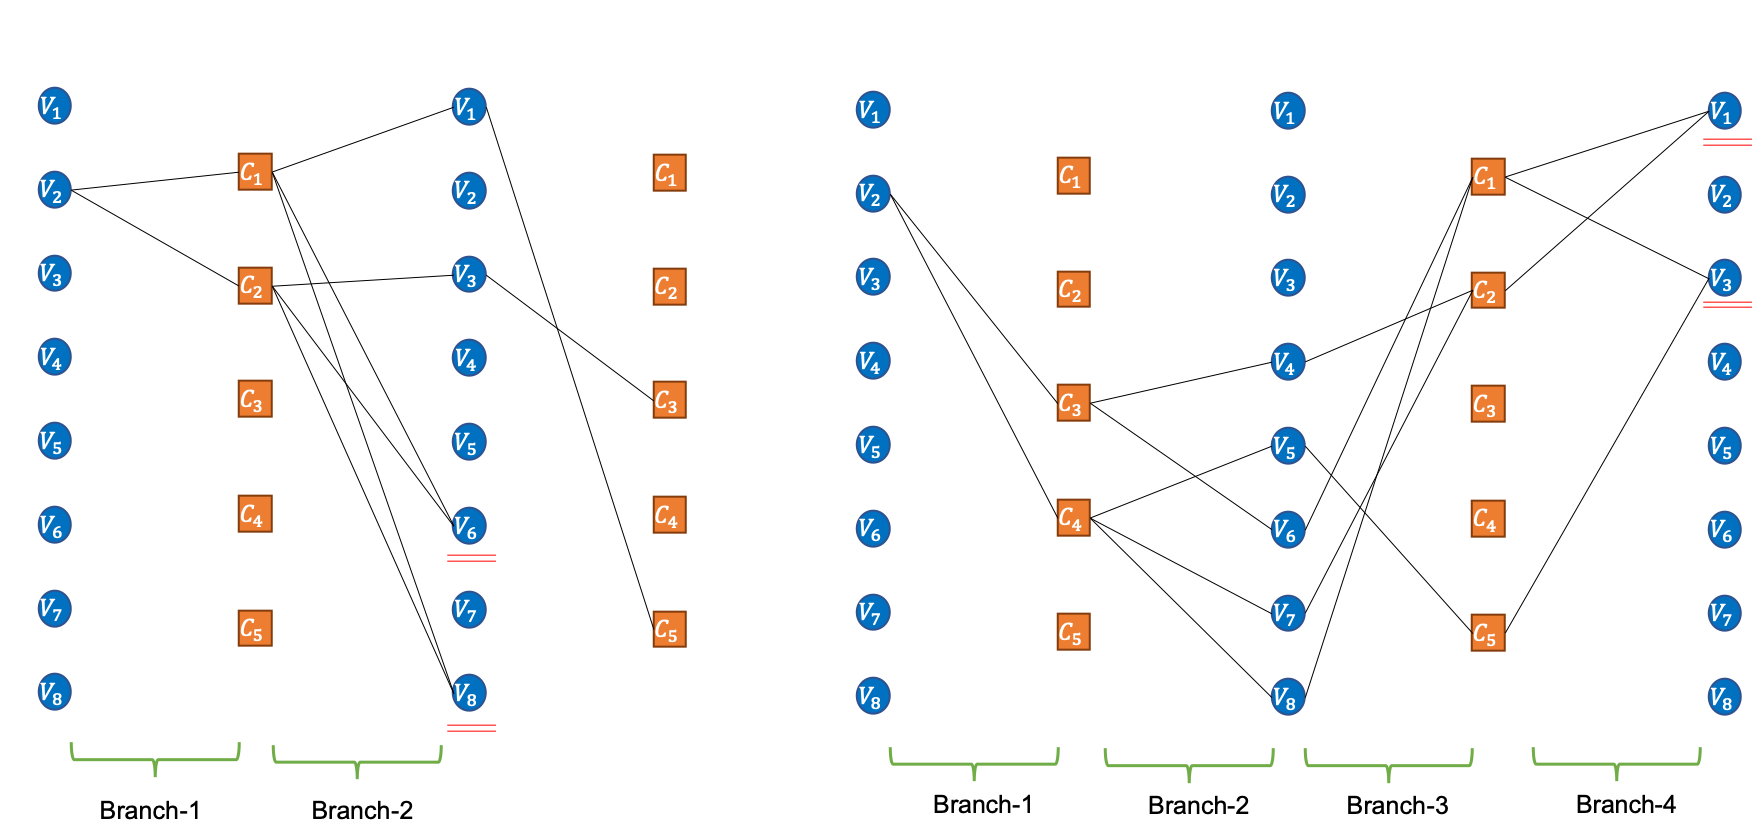
\includegraphics[width=1\textwidth]{pics/hitunggirth}
	\centering 
	\caption{Algoritma untuk menghitung \textit{girth} LDPC \textit{codes} yang diusulkan.}
	\label{fig:girthhitung}
\end{figure}
Tugas Akhir ini mengusulkan sebuah teknik untuk menghitung \textit{girth} dari setiap \textit{variable nodes} pada LDPC \textit{codes}, sehingga dapat diketahui distribusi \textit{local girth} dari LDPC \textit{codes}. \textit{Girth} adalah nilai \textit{local girth} terkecil dari distribusi \textit{girth} LDPC \textit{codes}. Teknik yang diusulkan adalah hasil dari modifikasi dan pengembangan dari algoritma pembuatan graf pohon pada PEG ditunjukkan oleh Gambar \ref{fig:girthhitung}. Berikut langkah-langkah untuk menghitung \textit{girth} yang diusulkan:
\begin{enumerate}
	\item Tentukan satu \textit{variable node} dan sebarkan \textit{edges}-nya sesuai dari matriks.
	\item Sebarkan \textit{edges} terus menerus sampai terdapat \textit{node} yang tidak dapat menyebarkan \textit{edge}.
	\item Hitung \textit{branch} $b$ dimulai dari satu, lalu dengan menggunakan persamaan
	\begin{equation}
	g=b\times 2,
	\end{equation}
	maka nilai \textit{local girth} $g$ dapat diketahui.
\end{enumerate}

% Bab 4 : Pengujian
%-----------------------------------------------------------------------------%
\chapter{\babEmpat}
%-----------------------------------------------------------------------------%
Bab ini menunjukkan hasil dari studi kinerja LDPC \textit{codes} DVB-T2 pada kanal AWGN dan \textit{channel model} DVB-T2 Indonesia. Bab ini juga menganalisis \textit{degree distribution} LDPC \textit{codes} DVB-T2 yang diusulkan dengan menggunakan EXIT \textit{chart} beserta validasinya menggunakan parameter praktis BER dan jumlah \textit{girth}.



\section{Analisis EXIT \textit{Chart} LDPC \textit{Codes} DVB-T2 pada Kanal AWGN}

Tugas Akhir ini menganalisis kinerja LDPC \textit{codes} DVB-T2 menggunakan EXIT \textit{chart} berdasarkan \textit{degree distribution} setiap \textit{code rate} dari LDPC \textit{codes} yang terbentuk. EXIT \textit{chart} mengeplot \textit{mutual information} di titik $V$ dan $C$ yang ditunjukkan pada proses \textit{iterative decoding} LDPC \textit{codes}. Secara praktis informasi ini diwakili oleh LLR, \textit{iterative decoding} pada LDPC \textit{codes} menukar LLR antara VND dan CND melalui \textit{edge} yang menghubungkan keduanya. \textit{Mutual information} yang terlibat adalah $ I_ {A, C} , I_ {E, C} , I_ {A, V} , I_ {E, V} $ seperti pada Gambar \ref{gambar: exit2} dan \ref{fig:exit49} mengekspresikan \textit{mutual information} yang masuk ke CND, \textit{mutual information} yang keluar dari CND, \textit{mutual information} yang masuk ke VND, dan \textit{mutual information} yang keluar dari VND pada iterasi LDPC \textit{codes}. Gambar \ref{gambar: exit2} menunjukkan EXIT \textit{chart} untuk \textit{code rate} $R_e=\frac{4}{9}$ untuk semua LDPC \textit{codes} DVB-T2 yang diusulkan pada SNR $\gamma=2.25$~dB dan menunjukkan EXIT \textit{chart} untuk \textit{code rate} $R_e=\frac{3}{5}$ untuk semua LDPC \textit{codes} DVB-T2 yang diusulkan pada SNR $\gamma=3.75$~dB. Gambar \ref{fig:exit49} menunjukkan EXIT \textit{chart} untuk \textit{code rate} $R_e=\frac{2}{3}$ untuk semua LDPC \textit{codes} DVB-T2 yang diusulkan pada SNR $\gamma=4$~dB.



Tugas Akhir ini mengalisis EXIT \textit{chart} pada setiap LDPC \textit{codes} DVB-T2 yang diusulkan pada kanal AWGN dalam dua dimensi (2D). Untuk mempermudah analisis, Tugas Akhir ini mengukur \textit{mutual information} menggunakan fungsi $J$ dan $J^{-1}$. Hubungan antara varians dan \textit{mutual information} adalah \cite{exit1}

\begin{eqnarray}
\sigma &=& J^{-1}({I_{A}}),\\
I&=&J(\sigma)
\end{eqnarray}
\begin{figure}
	\centering
	%	\hspace{-0.2 in}
	\begin{minipage}{1\linewidth}
		\hspace{0.75 cm}
		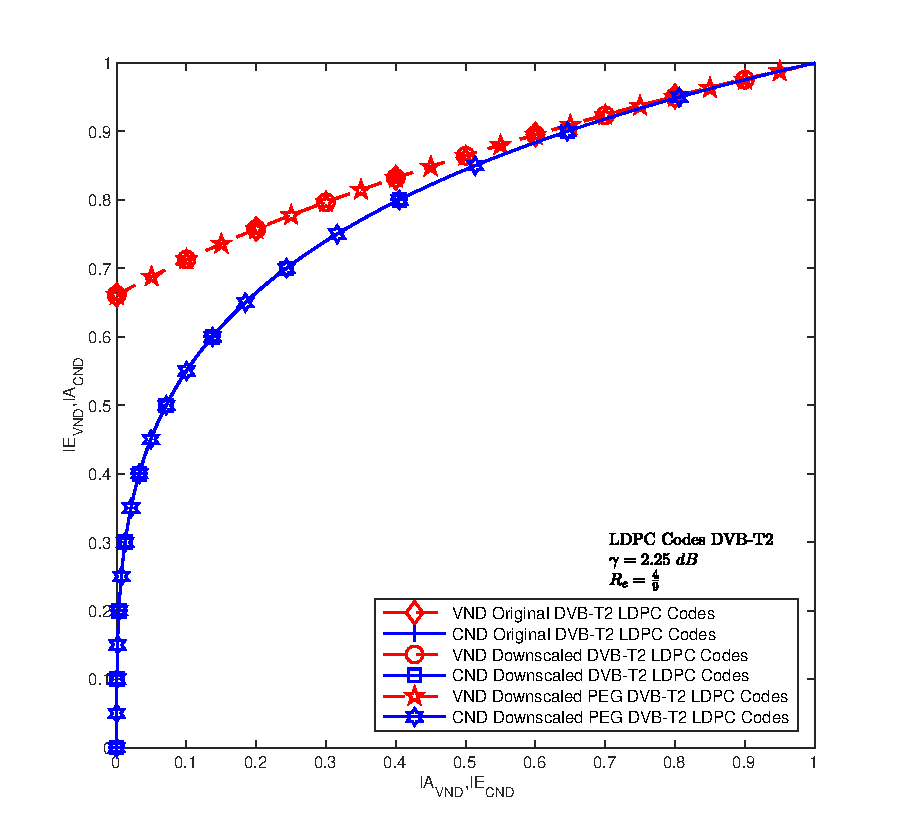
\includegraphics[width=0.85\textwidth]{pics/exit/12/12semua=snr2,25Ich=0,6613.pdf}
		\vspace{-1cm}
		
		\center  (a)
	\end{minipage}
	\hfill
	\begin{minipage}{1\linewidth}
		\hspace{0.75 cm}
		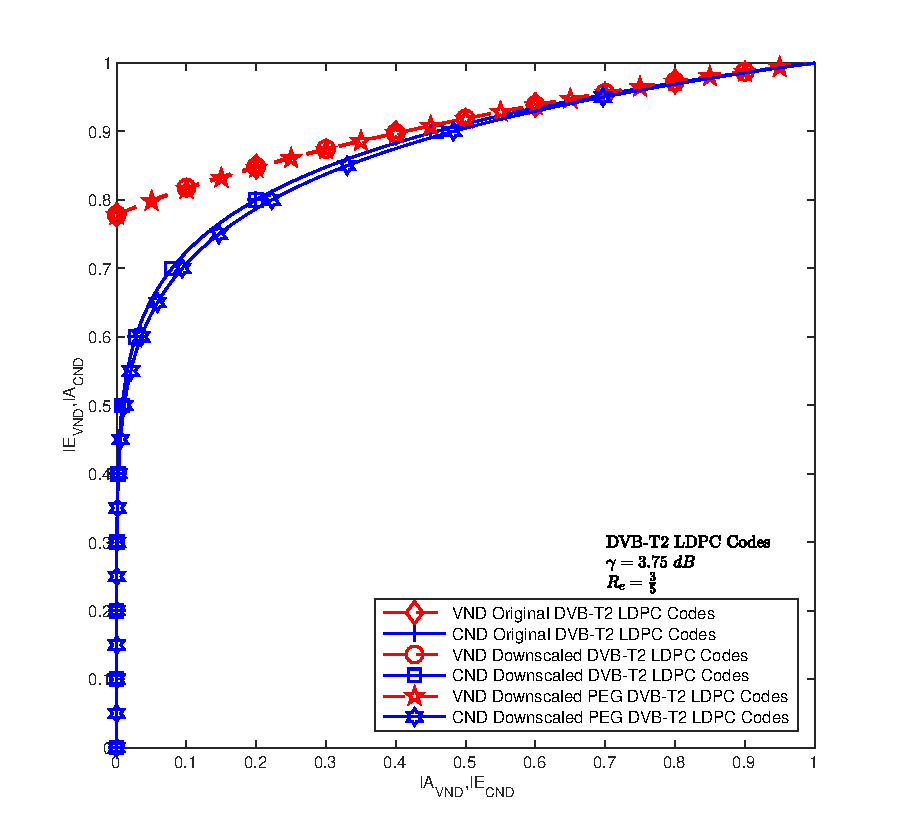
\includegraphics[width=0.85\textwidth]{pics/exit/35/35semua=snr3,75Ich=0,7786.pdf}
		\vspace{-1cm}
		\center (b)
	\end{minipage}
	%	\begin{minipage}{.5\linewidth}
	%		\hspace{-0.4 cm}
	%		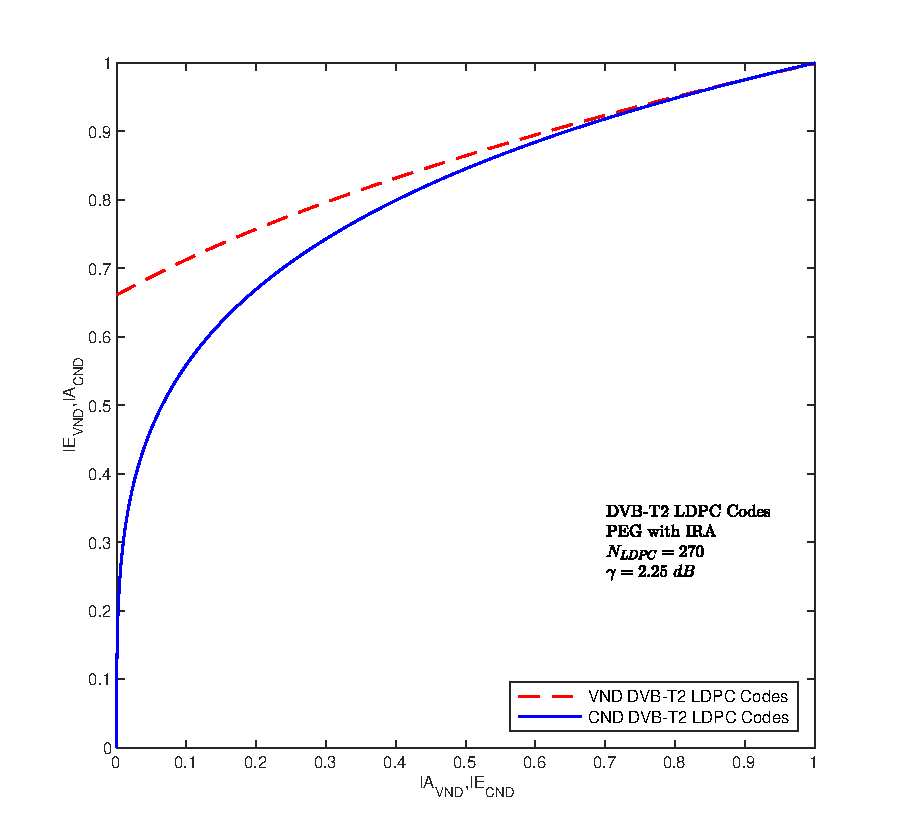
\includegraphics[width=3in]{pics/exit/12/12peg=snr2,25Ich=0,6613.pdf}
	%		\vspace{-1cm}
	%		\center (c)
	%	\end{minipage}
	\caption {Analisis EXIT \textit{chart} LDPC \textit{codes} DVB-T2 dengan (a) $R_e=\frac{4}{9}$ dan (b) $R_e=\frac{3}{5}$, masing-masing, pada SNR $\gamma=2,5~dB$ dan $\gamma=3,75~dB$.}
	\label{gambar: exit2}
\end{figure}\begin{figure}[t!]
\centering
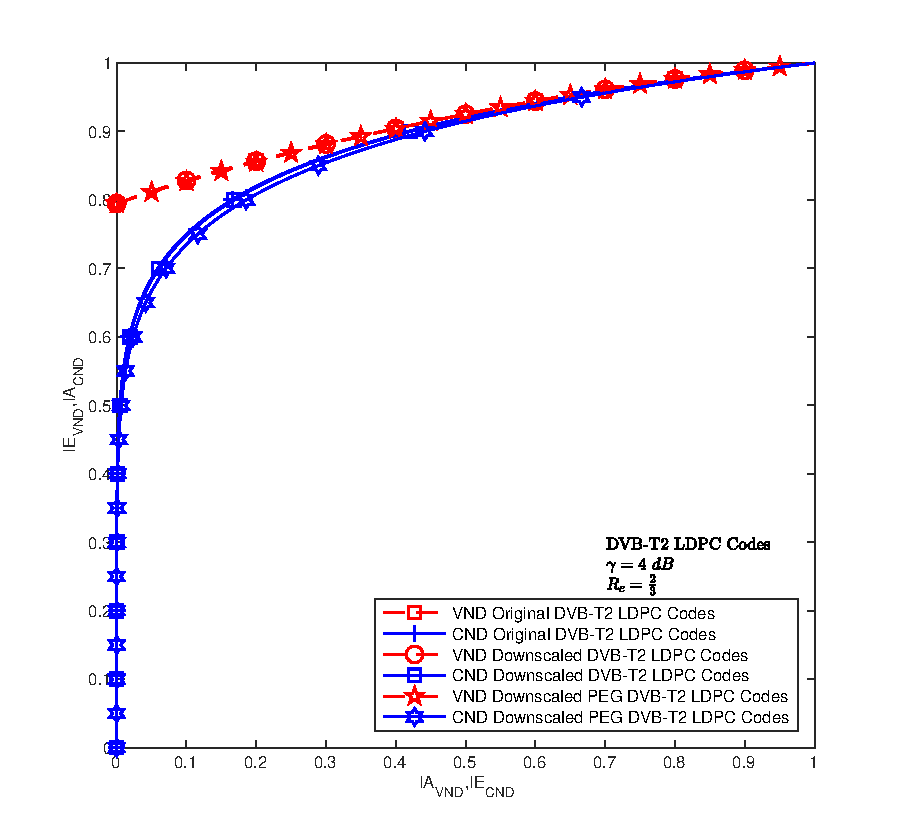
\includegraphics[width=1\textwidth]
{pics/exit/23/23semua=snr4Ich=0,795.pdf}
\caption{Analisis EXIT \textit{chart} LDPC \textit{codes} DVB-T2 dengan $R_e=\frac{2}{3}$ pada SNR $\gamma=4~dB$.}
\label{fig:exit49}
\end{figure} 
\noindent dengan $\sigma^2 = \frac{4}{\sigma_n^2}$,  $\sigma_n^2$ adalah \textit{noise variance}.  EXIT \textit{chart} dalam Tugas Akhir ini mengeplot berdasarkan \textit{mutual information}
\begin{equation}
I_{E,V}\! =\! \sum_i \mathcal{F}_i^\Lambda { J\left( \sqrt{(d_{V_i}\!-\!1)[J^{-1}(I_{A,V})]^2\!+\! [J^{-1}(I_{A_{CH}})]^2}\right)}
\label{eq:I_E_V_int}
\end{equation} 
dengan $\mathcal{F}_i^\Lambda$ adalah pecahan ke-$i$ dari $\Lambda_{LDPC}(x)$ dan 
\begin{equation}
I_{E,C} = 1-\sum_i \mathcal{F}_i^\Omega J\left( \sqrt{(d_{C_i}-1)[J^{-1}(1-I_{A,C})]^2}\right)
\end{equation}
dengan $\mathcal{F}_i^\Omega$ adalah pecahan ke-$i$ pada $\Omega_{LDPC}(x)$. Parameter $I_{A_{CH}}$ adalah \textit{mutual information} yang berasal dari \textit{channel}.


Gambar \ref{fig:exit3} menunjukkan EXIT \textit{chart} untuk \textit{code rate} $R_e=\frac{11}{15}$ untuk semua LDPC \textit{codes} DVB-T2 yang diusulkan pada SNR $\gamma=4.25$~dB. Gambar \ref{gambar: exit737} menunjukkan EXIT \textit{chart} untuk \textit{code rate} $R_e=\frac{11}{15}$ untuk semua LDPC \textit{codes} DVB-T2 yang diusulkan pada SNR $\gamma=4.5$~dB dan menunjukkan EXIT \textit{chart} untuk \textit{code rate} $R_e=\frac{37}{45}$ untuk semua LDPC \textit{codes} DVB-T2 yang diusulkan pada SNR $\gamma=5.25$~dB.

EXIT \textit{chart} menunjukkan celah kecil yang membuktikan distribusi derajat yang baik, celah terbuka pada EXIT \textit{chart} bermanfaat untuk memulai decoding di awal kurva. Evaluasi EXIT \textit{chart} pada Tugas Akhir ini menunjukkan semakin besar \textit{code rate}, maka nilai SNR untuk mencapai kurva EXIT yang baik semakin besar. Setiap kurva EXIT \textit{chart} menunjukkan bahwa original LDPC \textit{codes} memiliki EXIT \textit{chart} yang sedikit lebih baik daripada LDPC \textit{codes} DVB-T2 yang diusulkan, sehingga membuktikan bahwa \textit{downscaled} LDPC \textit{codes} dapat memiliki kinerja yang tidak jauh beda daripada original LDPC \textit{codes}.
\begin{figure}[b!]
	\centering
	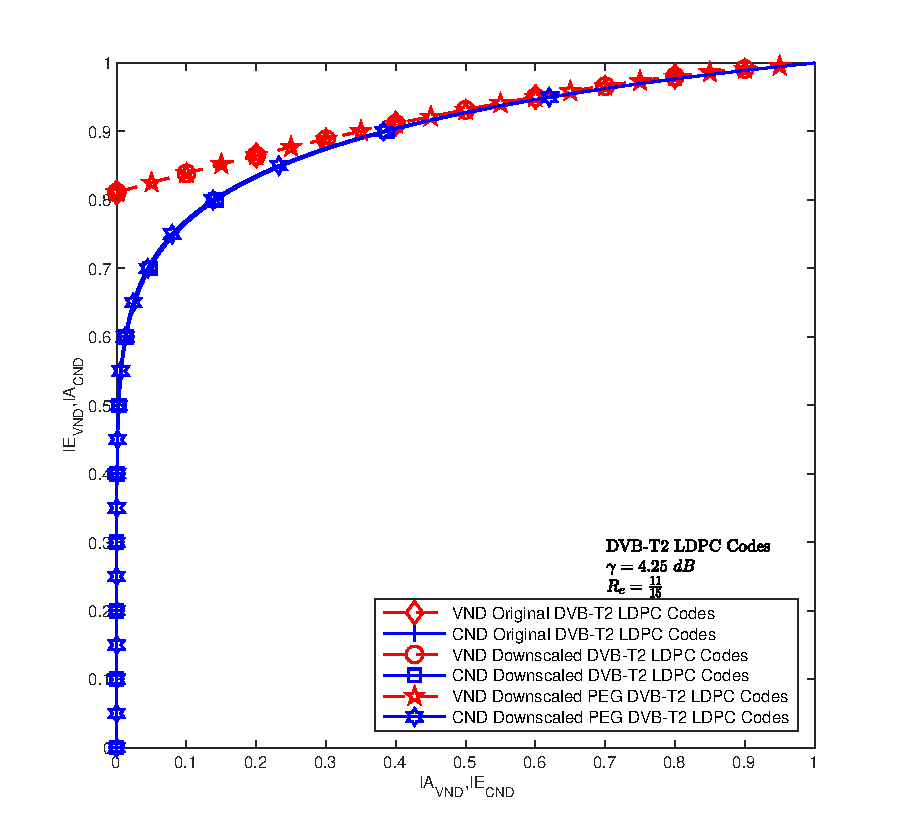
\includegraphics[width=1\textwidth]
	{pics/exit/34/34semua=snr4,25Ich=0,8113.pdf}
	\caption{Analisis EXIT \textit{chart} LDPC \textit{codes} DVB-T2 dengan $R_e=\frac{11}{15}$ pada SNR $\gamma=4,25~dB$.}
	\label{fig:exit3}
\end{figure}
\begin{figure}[H]
	\centering
	%	\hspace{-0.2 in}
	\begin{minipage}{1\linewidth}
		\hspace{0.75 cm}
		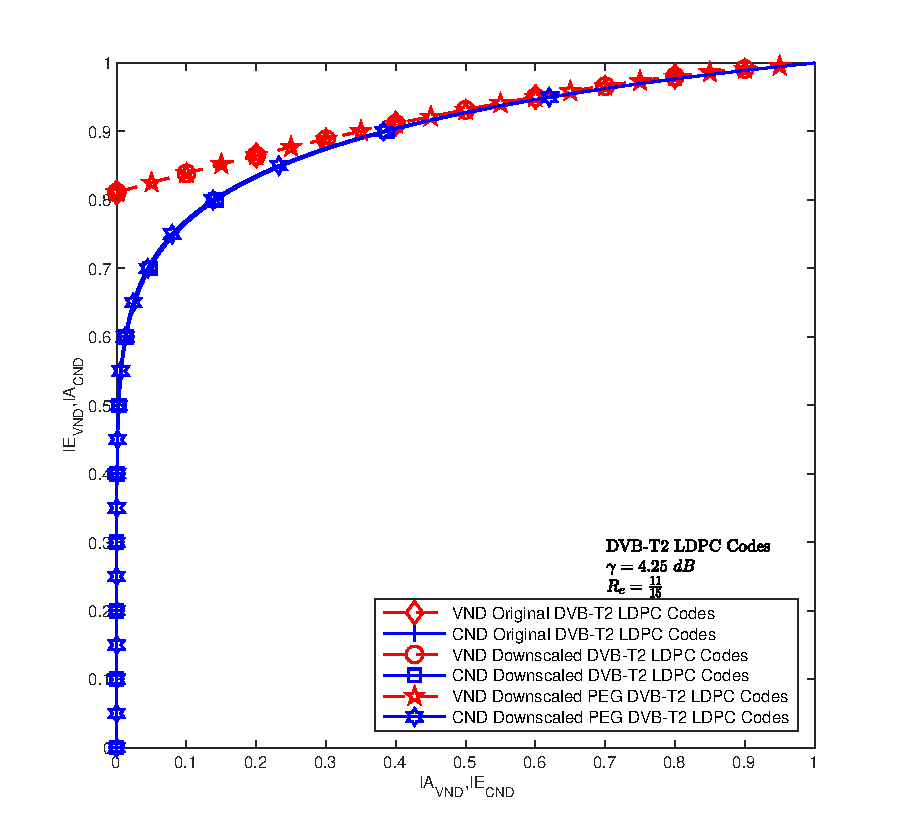
\includegraphics[width=0.85\textwidth]{pics/exit/34/34semua=snr4,25Ich=0,8113.pdf}
		\vspace{-1cm}
		
		\center  (a)
	\end{minipage}
	\hfill
	\begin{minipage}{1\linewidth}
		\hspace{0.75 cm}
		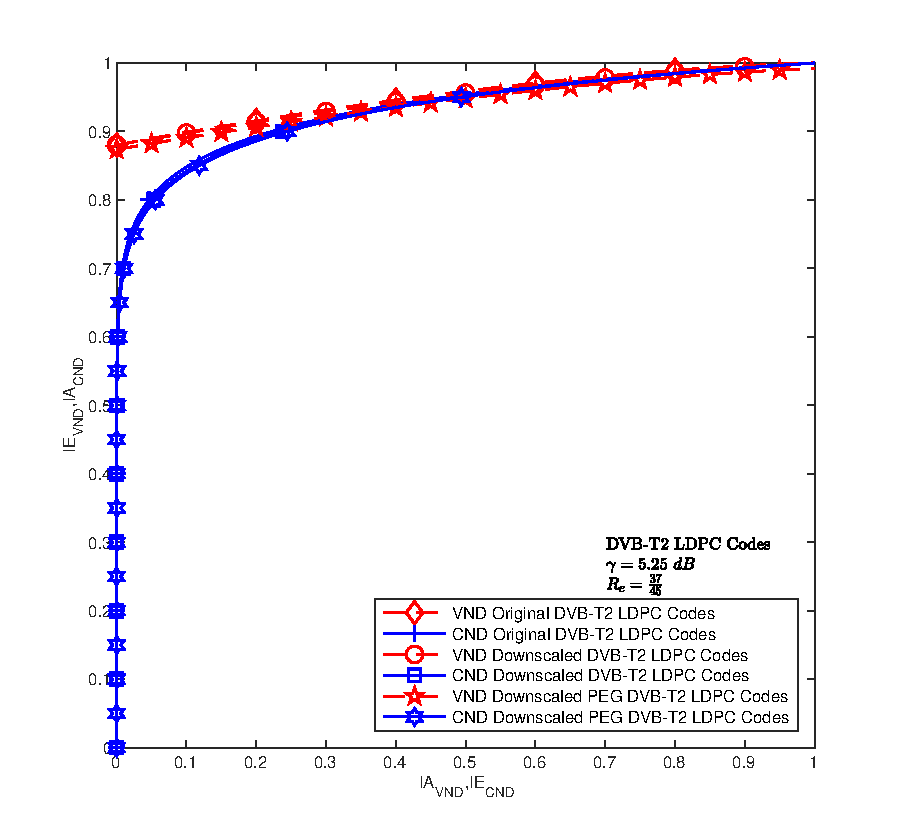
\includegraphics[width=0.85\textwidth]{pics/exit/56/56semua=snr5,25Ich=0,8804.pdf}
		\vspace{-1cm}
		\center (b)
	\end{minipage}
	%	\begin{minipage}{.5\linewidth}
	%		\hspace{-0.4 cm}
	%		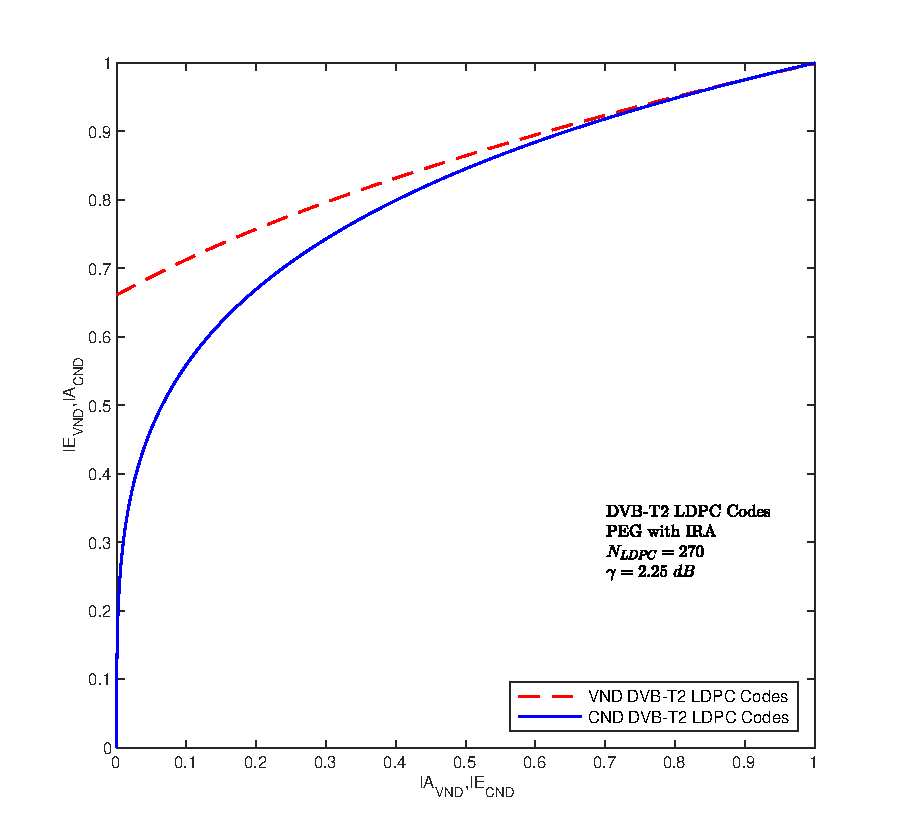
\includegraphics[width=3in]{pics/exit/12/12peg=snr2,25Ich=0,6613.pdf}
	%		\vspace{-1cm}
	%		\center (c)
	%	\end{minipage}
	\caption {Analisis EXIT \textit{chart} LDPC \textit{codes} DVB-T2 pada (a) $R_e=\frac{7}{9}$ dan (b) $R_e=\frac{37}{45}$, masing-masing, pada SNR $\gamma=4,5~dB$ dan $\gamma=5,25~dB$.}
	\label{gambar: exit737}
\end{figure}






%-----------------------------------------------------------------------------%

%EXIT
%\hspace{15cm}
%\begin{figure}
%	\centering
%	\hspace{-0.1 in}
%	\begin{minipage}{.5\linewidth}
%		\hspace{-0.5cm}
%		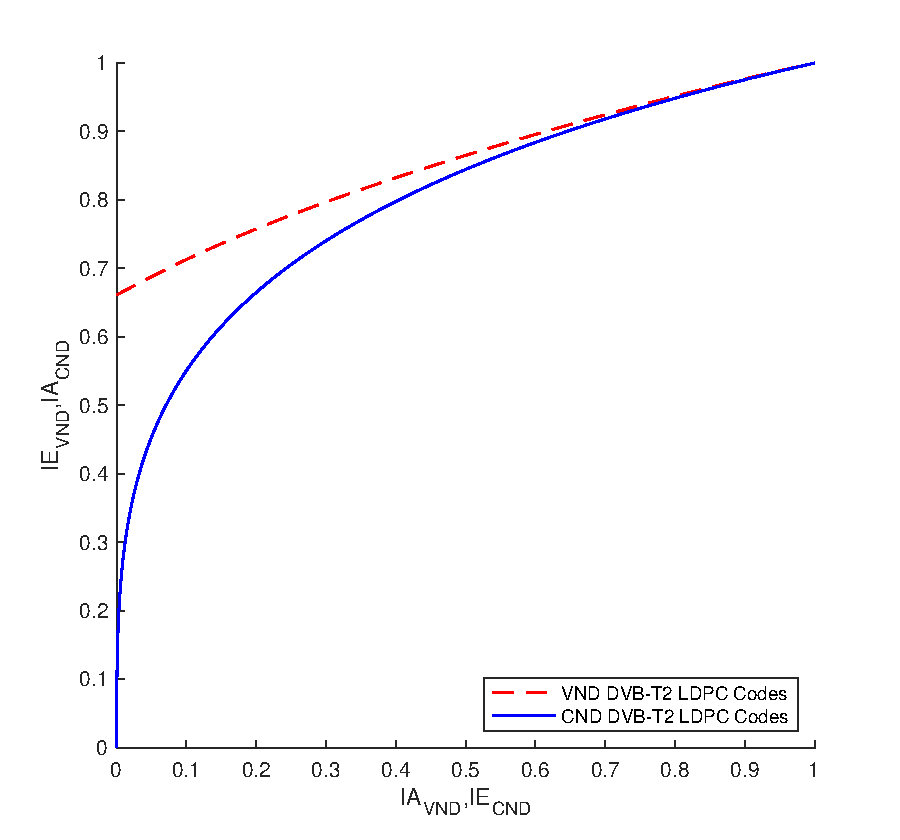
\includegraphics[width=3in]{pics/12/12asli=snr2,25Ich=0,6613.pdf}
%		\vspace{-1.25cm}
%		
%		\center (a)
%	\end{minipage}
%	\hfill 	\hspace{-0.1 in}
%	\begin{minipage}{.5\linewidth}
%%		\hspace{2.25 cm}
%		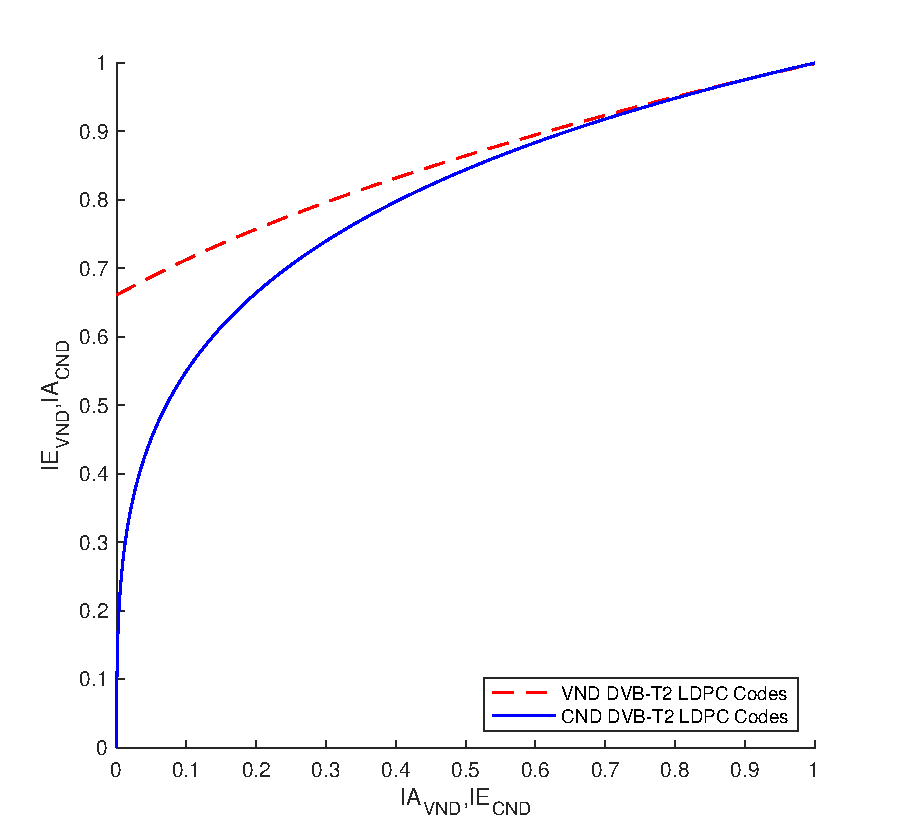
\includegraphics[width=3in]{pics/12/12ds=snr2,25Ich=0,6613.pdf}
%		\vspace{-1.15cm}
%		\center \hspace*{0.75cm}(b)
%	\end{minipage}
%	\begin{minipage}{.5\linewidth}
%		\hspace{-0.5cm}
%		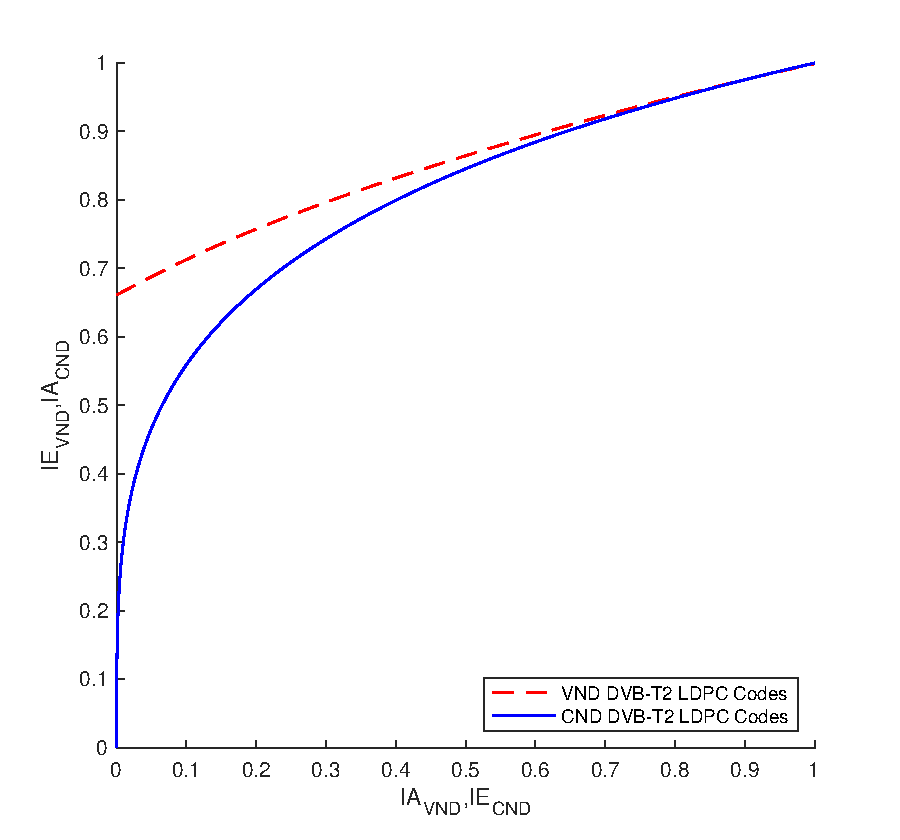
\includegraphics[width=3in]{pics/12/12peg=snr2,25Ich=0,6613.pdf}
%		\vspace{-1.25cm}
%		\center (c)
%	\end{minipage}
%	\hspace{-0.1 in}
%	\begin{minipage}{.5\linewidth}
%%		\hspace{2.25 cm}
%		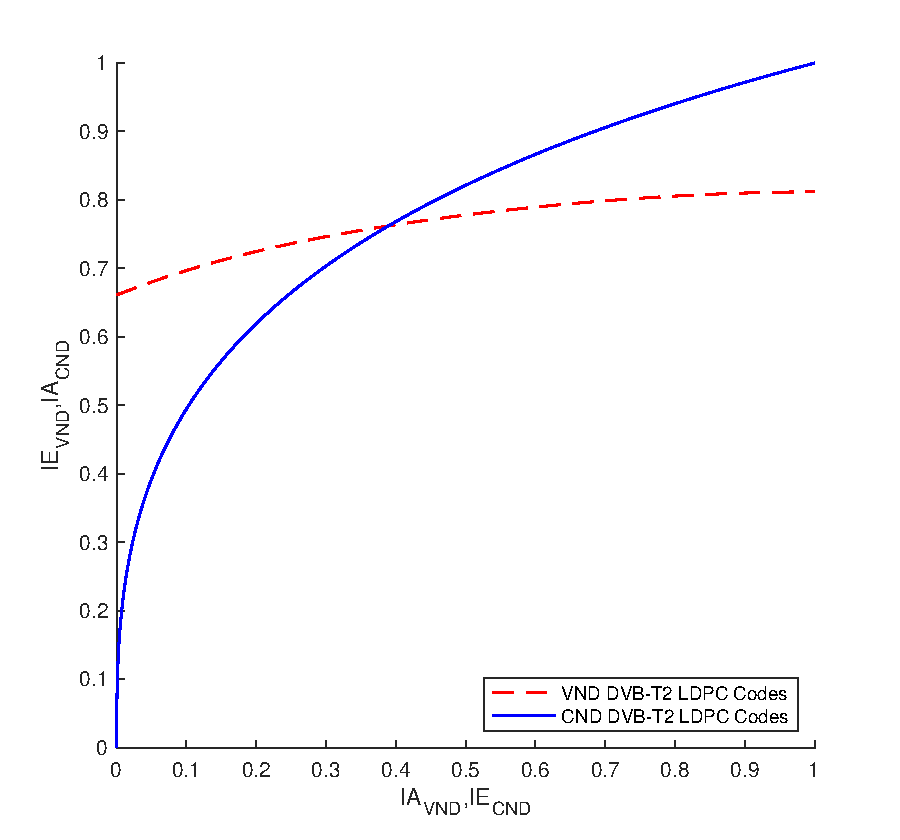
\includegraphics[width=3in]{pics/12/12pegLDGM=snr2,25Ich=0,6613.pdf}
%		\vspace{-1.25cm}
%		\center \hspace*{0.75cm}(d)
%	\end{minipage}
%	\caption {Analisis EXIT \textit{Chart} LDPC \textit{codes} DVB-T2 $R_e=\frac{4}{9}$ dengan: (a)  $N_{LDPC}=16200$, (b) $N_{LDPC}=270$ menggunakan metode \textit{downscaled}, (c) $N_{LDPC}=270$ menggunakan PEG dengan \textit{accumulator}, dan (d) $N_{LDPC} = 270 $ menggunakan PEG dengan LDGM.}
%	\label{gambar: exit49}
%\end{figure}



%
%\begin{figure}
%	\centering
%	\hspace{-0.2 in}
%	\begin{minipage}{.5\linewidth}
%		\hspace{-0.4 cm}
%		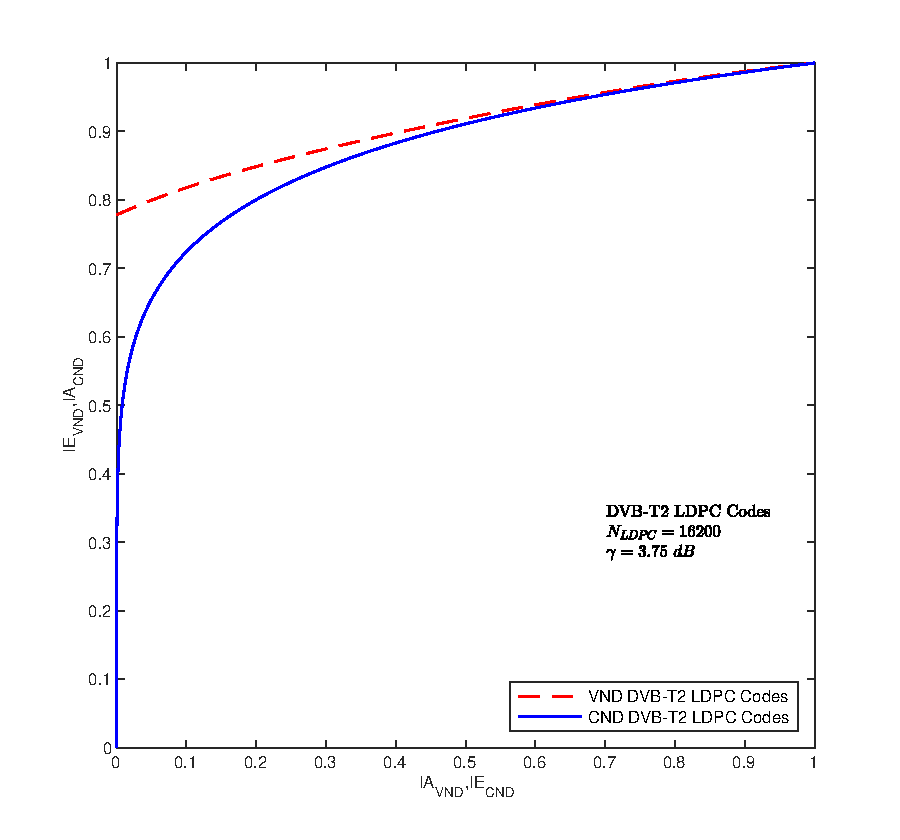
\includegraphics[width=3in]{pics/exit/35/35asli=snr3,75Ich=0,7786.pdf}
%		\vspace{-1cm}
%		
%		\center (a)
%	\end{minipage}
%	\hfill
%	\begin{minipage}{.5\linewidth}
%		\hspace{-0.4 cm}
%		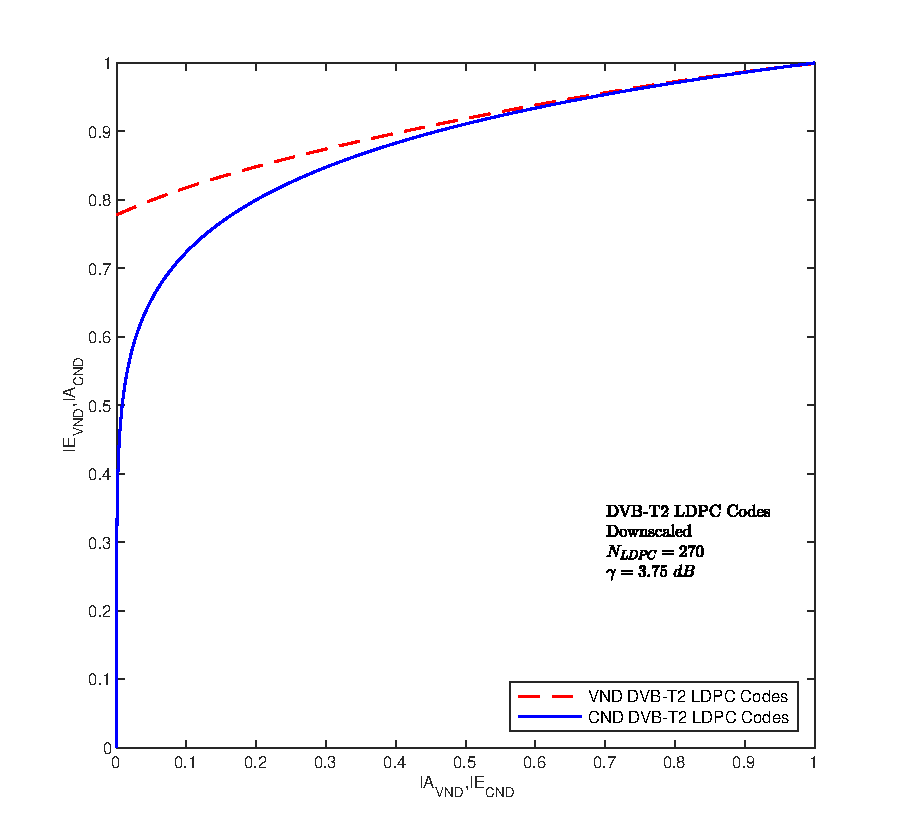
\includegraphics[width=3in]{pics/exit/35/35ds=snr3,75Ich=0,7786.pdf}
%		\vspace{-1cm}
%		\center (b)
%	\end{minipage}
%	\begin{minipage}{.5\linewidth}
%		\hspace{-0.4 cm}
%		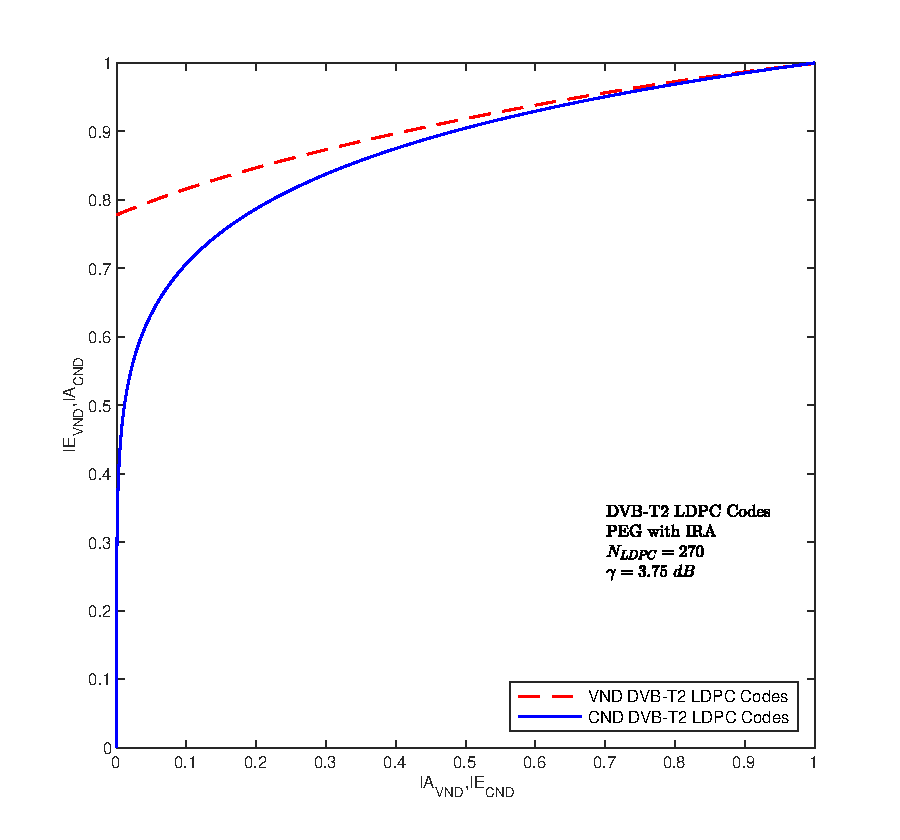
\includegraphics[width=3in]{pics/exit/35/35peg=snr3,75Ich=0,7786.pdf}
%		\vspace{-1cm}
%		\center (c)
%	\end{minipage}
%%		\caption {Analisis EXIT \textit{Chart} LDPC \textit{codes} DVB-T2 $R_e=\frac{3}{5}$ dengan: (a)  $N_{LDPC}=16200$, (b) $N_{LDPC}=270$ menggunakan metode \textit{downscaled}, dan (c) $N_{LDPC}=270$ menggunakan PEG.}
%	\caption {Analisis EXIT \textit{Chart} LDPC \textit{codes} DVB-T2 $R_e=\frac{3}{5}$.}
%	\label{gambar: exit35}
%\end{figure}
%
%\begin{figure}
%	\centering
%	\hspace{-0.2 in}
%	\begin{minipage}{.5\linewidth}
%		\hspace{-0.4 cm}
%		\includegraphics[width=3in]{pics/exit/23/23asli=snr4Ich=0,795.pdf}
%		\vspace{-1cm}
%		
%		\center (a)
%	\end{minipage}
%	\hfill
%	\begin{minipage}{.5\linewidth}
%		\hspace{-0.4 cm}
%		\includegraphics[width=3in]{pics/exit/23/23ds=snr4Ich=0,795.pdf}
%		\vspace{-1cm}
%		\center (b)
%	\end{minipage}
%	\begin{minipage}{.5\linewidth}
%		\hspace{-0.4 cm}
%		\includegraphics[width=3in]{pics/exit/23/23peg=snr4Ich=0,795.pdf}
%		\vspace{-1cm}
%		\center (c)
%	\end{minipage}
%%		\caption {Analisis EXIT \textit{Chart} LDPC \textit{codes} DVB-T2 $R_e=\frac{2}{3}$ dengan: (a)  $N_{LDPC}=16200$, (b) $N_{LDPC}=270$ menggunakan metode \textit{downscaled}, dan (c) $N_{LDPC}=270$ menggunakan PEG.}
%			\caption {Analisis EXIT \textit{Chart} LDPC \textit{codes} DVB-T2 $R_e=\frac{2}{3}$.}
%	\label{gambar: exit23}
%\end{figure}
%
%\begin{figure}
%	\centering
%	\hspace{-0.2 in}
%	\begin{minipage}{.5\linewidth}
%		\hspace{-0.4 cm}
%		\includegraphics[width=3in]{pics/exit/34/34asli=snr4,25Ich=0,8113.pdf}
%		\vspace{-1cm}
%		
%		\center (a)
%	\end{minipage}
%	\hfill
%	\begin{minipage}{.5\linewidth}
%		\hspace{-0.4 cm}
%		\includegraphics[width=3in]{pics/exit/34/34asli=snr4,25Ich=0,8113.pdf}
%		\vspace{-1cm}
%		\center (b)
%	\end{minipage}
%	\begin{minipage}{.5\linewidth}
%		\hspace{-0.4 cm}
%		\includegraphics[width=3in]{pics/exit/34/34asli=snr4,25Ich=0,8113.pdf}
%		\vspace{-1cm}
%		\center (c)
%	\end{minipage}
%%		\caption {Analisis EXIT \textit{Chart} LDPC \textit{codes} DVB-T2 $R_e=\frac{11}{15}$ dengan: (a)  $N_{LDPC}=16200$, (b) $N_{LDPC}=270$ menggunakan metode \textit{downscaled}, dan (c) $N_{LDPC}=270$ menggunakan PEG.}
%		\caption {Analisis EXIT \textit{Chart} LDPC \textit{codes} DVB-T2 $R_e=\frac{11}{15}$.}
%	\label{gambar: exit1115}
%\end{figure}
%
%\begin{figure}
%	\centering
%	\hspace{-0.2 in}
%	\begin{minipage}{.5\linewidth}
%		\hspace{-0.4 cm}
%		\includegraphics[width=3in]{pics/exit/45/45asli=snr4,5Ich=0,8303.pdf}
%		\vspace{-1cm}
%		
%		\center (a)
%	\end{minipage}
%	\hfill
%	\begin{minipage}{.5\linewidth}
%		\hspace{-0.4 cm}
%		\includegraphics[width=3in]{pics/exit/45/45ds=snr4,5Ich=0,8303.pdf}
%		\vspace{-1cm}
%		\center (b)
%	\end{minipage}
%	\begin{minipage}{.5\linewidth}
%		\hspace{-0.4 cm}
%		\includegraphics[width=3in]{pics/exit/45/45peg=snr4,5Ich=0,8303.pdf}
%		\vspace{-1cm}
%		\center (c)
%	\end{minipage}
%%		\caption {Analisis EXIT \textit{Chart} LDPC \textit{codes} DVB-T2 $R_e=\frac{7}{9}$ dengan: (a)  $N_{LDPC}=16200$, (b) $N_{LDPC}=270$ menggunakan metode \textit{downscaled}, dan (c) $N_{LDPC}=270$ menggunakan PEG.}
%		\caption {Analisis EXIT \textit{Chart} LDPC \textit{codes} DVB-T2 $R_e=\frac{7}{9}$.}
%	\label{gambar: exit79}
%\end{figure}
%
%\begin{figure}
%	\centering
%	\hspace{-0.2 in}
%	\begin{minipage}{.5\linewidth}
%		\hspace{-0.4 cm}
%		\includegraphics[width=3in]{pics/exit/56/56asli=snr5,25Ich=0,8804.pdf}
%		\vspace{-1cm}
%		
%		\center (a)
%	\end{minipage}
%	\hfill
%	\begin{minipage}{.5\linewidth}
%		\hspace{-0.4 cm}
%		\includegraphics[width=3in]{pics/exit/56/56ds=snr5,25Ich=0,8804.pdf}
%		\vspace{-1cm}
%		\center (b)
%	\end{minipage}
%	\begin{minipage}{.5\linewidth}
%		\hspace{-0.4 cm}
%		\includegraphics[width=3in]{pics/exit/56/56peg=snr5,25Ich=0,8804.pdf}
%		\vspace{-1cm}
%		\center (c)
%	\end{minipage}
%%	\caption {Analisis EXIT \textit{Chart} LDPC \textit{codes} DVB-T2 $R_e=\frac{37}{45}$ dengan: (a)  $N_{LDPC}=16200$, (b) $N_{LDPC}=270$ menggunakan metode \textit{downscaled}, dan (c) $N_{LDPC}=270$ menggunakan PEG.}
%		\caption {Analisis EXIT \textit{Chart} LDPC \textit{codes} DVB-T2 $R_e=\frac{37}{45}$.}
%\label{gambar: exit3745}
%\end{figure}










% Gambar \ref{gambar: exit49} menunjukkan perbandingan EXIT \textit{chart} antara original, \textit{downscaled}, dan \textit{downscaled} menggunakan PEG DVB-T2 LDPC \textit{codes} dengan code rate $R_e=\frac{4}{9}$ pada SNR $\gamma=2,25$. Gambar \ref{gambar: exit35} menunjukkan perbandingan EXIT \textit{chart} antara original, \textit{downscaled}, dan \textit{downscaled} menggunakan PEG DVB-T2 LDPC \textit{codes} dengan code rate $R_e=\frac{3}{5}$ pada SNR $\gamma=3,75$. Gambar \ref{gambar: exit23} menunjukkan perbandingan EXIT \textit{chart} antara original, \textit{downscaled}, dan \textit{downscaled} menggunakan PEG DVB-T2 LDPC \textit{codes} dengan code rate $R_e=\frac{2}{3}$ pada SNR $\gamma=4$. Gambar \ref{gambar: exit1115} menunjukkan perbandingan EXIT \textit{chart} antara original, \textit{downscaled}, dan \textit{downscaled} menggunakan PEG DVB-T2 LDPC \textit{codes} dengan code rate $R_e=\frac{11}{15}$ pada SNR $\gamma=4,25$. Gambar \ref{gambar: exit79} menunjukkan perbandingan EXIT \textit{chart} antara original, \textit{downscaled}, dan \textit{downscaled} menggunakan PEG DVB-T2 LDPC \textit{codes} dengan code rate $R_e=\frac{7}{9}$ pada SNR $\gamma=4,5$. Gambar \ref{gambar: exit3745} menunjukkan perbandingan EXIT \textit{chart} antara original, \textit{downscaled}, dan \textit{downscaled} menggunakan PEG DVB-T2 LDPC \textit{codes} dengan code rate $R_e=\frac{37}{45}$ pada SNR $\gamma=5,25$.

 %-----------------------------------------------------------------------------%

\section{Analisis Kinerja BER}
Tugas Akhir ini mengevaluasi kinerja BER dari LDPC \textit{codes} DVB-T2 dengan $N_{LDPC}=16200$, \textit{downscaled} LDPC \textit{codes} DVB-T2 dengan $N_{LDPC}=270$, \textit{downscaled} LDPC \textit{codes} DVB-T2 menggunakan PEG dengan \textit{accumulator}, dan \textit{downscaled} LDPC \textit{codes} DVB-T2 menggunakan PEG dengan LDGM pada kanal AWGN dan \textit{channel model} DVB-T2 Indonesia.
% yang direpresentasikan oleh \textit{channel model} DVB-T2 Kota Bandung.


%\begin{figure}
%	\centering
%	\hspace{ -0.1in}
%	\begin{minipage}{.5\linewidth}
%		\hspace{-1.15cm}
%		\includegraphics[width=3.5in]{pics/exit/23/23semua=snr4Ich=0,795.pdf}
%		\vspace{-1.5cm}
%		
%		\center (a)
%	\end{minipage}
%	\hfill 	\hspace{ -0.1in}
%	\begin{minipage}{.5\linewidth}
%%		\hspace{2.25 cm}
%		\includegraphics[width=3.5in]{pics/exit/34/34semua=snr4,25Ich=0,8113.pdf}
%		
%		\vspace{-0.95cm}
%		\center \hspace*{2.25cm}(b)
%	\end{minipage}
%	
%	\begin{minipage}{.5\linewidth}
%		\hspace{-1.25cm}
%		\includegraphics[width=3.5in]{pics/exit/45/45semua=snr4,5Ich=0,8303.pdf}
%		\vspace{-1.5cm}
%		\center (c)
%	\end{minipage}
%	\hfill \hspace{-0.1 in}
%	\begin{minipage}{.5\linewidth}
%%		\hspace{2.25 cm}
%		\includegraphics[width=3.5in]{pics/exit/56/56semua=snr5,25Ich=0,8804.pdf}
%		\vspace{-1.5cm}
%		\center \hspace*{2.25cm}(d)
%	\end{minipage}
%	\caption {Analisis EXIT \textit{chart} LDPC \textit{codes} DVB-T2 pada (a) $R_e=\frac{2}{3}$, (b) $R_e=\frac{11}{15}$, (c) $R_e=\frac{7}{9}$, dan (d) $R_e=\frac{37}{45}$.}
%	\label{gambar: exit4}
%\end{figure}


%\begin{figure}
%	\centering
%	\hspace{-0.2 in}
%	\begin{minipage}{.5\linewidth}
%		\hspace{-0.4 cm}
%		\includegraphics[width=3in]{hasildsfix.pdf}
%		\vspace{-1cm}
%		
%		\center (a)
%	\end{minipage}
%	\hfill
%	\begin{minipage}{.5\linewidth}
%		\hspace{-0.4 cm}
%		\includegraphics[width=3in]{hasilpegawgn.pdf}
%		\vspace{-1cm}
%		\center (b)
%	\end{minipage}
%	\hspace{-0.8 in}
%	\begin{minipage}{.5\linewidth}
%		\hspace{-0.4 cm}
%		\includegraphics[width=3in]{hasiloriAWGN.pdf}
%		\vspace{-1cm}
%		\center (c)
%	\end{minipage}
%	\begin{minipage}{.5\linewidth}
%	\hspace{2.25 cm}
%	\includegraphics[width=3in]{hasilpegawgnfixLDGM.pdf}
%	\vspace{-0.5cm}
%	\center (c)
%\end{minipage}
%	\caption {Kinerja BER LDPC \textit{codes} DVB-T2 dengan: (a) $N_{LDPC}=270$ menggunakan PEG, (b) $N_{LDPC}=270$ menggunakan metode \textit{downscaled}, dan (c) $N_{LDPC}=16200$ pada kanal AWGN .}
%	\label{gambar: awgnhasil}
%\end{figure}




\subsection{Kinerja pada Kanal AWGN}
Tugas Akhir ini membandingkan hasil kinerja BER dengan teori BER pada kanal AWGN dalam SNR $\gamma$ seperti pada Gambar \ref{fig:awgnori} dan \ref{gambar:dspeg}. 
\begin{figure}[b!]
	\centering
	\includegraphics[width=1\textwidth]
	{hasiloriAWGN.pdf}
	\caption{Kinerja BER LDPC \textit{codes} DVB-T2 dengan $N_{LDPC}=16200$ pada kanal AWGN.}
	\label{fig:awgnori}
\end{figure}


\begin{figure}[H]
	\centering
	%	\hspace{-0.2 in}
	\begin{minipage}{1\linewidth}
		\hspace{0.75 cm}
		\includegraphics[width=0.85\textwidth]{hasildsfix.pdf}
		\vspace{-1cm}
		
		\center  (a)
	\end{minipage}
	\hfill
	\begin{minipage}{1\linewidth}
		\hspace{0.75 cm}
		\includegraphics[width=0.85\textwidth]{hasilpegawgnfix.pdf}
		\vspace{-1cm}
		\center (b)
	\end{minipage}
	%	\begin{minipage}{.5\linewidth}
	%		\hspace{-0.4 cm}
	%		\includegraphics[width=3in]{pics/exit/12/12peg=snr2,25Ich=0,6613.pdf}
	%		\vspace{-1cm}
	%		\center (c)
	%	\end{minipage}
	\caption {Kinerja BER LDPC \textit{codes} DVB-T2 dengan: (a) $N_{LDPC}=270$ menggunakan metode \textit{downscaling} dan (b) $N_{LDPC}=270$ menggunakan PEG dengan \textit{accumulator} pada kanal AWGN.}
	\label{gambar:dspeg}
\end{figure}

Gambar \ref{fig:awgnori} menunjukkan perbandingan kinerja original LDPC \textit{codes} DVB-T2 untuk semua \textit{code rate} pada kanal AWGN dengan teori BER QPSK dan \textit{uncoded} QPSK, LDPC \textit{codes} DVB-T2 yang diusulkan terbukti dapat memiliki kinerja BER yang jauh lebih baik daripada teori BER QPSK dan tanpa \textit{channel coding} (\textit{uncoded}) QPSK. Gambar \ref{gambar:dspeg} (a) menunjukkan perbandingan kinerja \textit{downscaled} LDPC \textit{codes} DVB-T2 untuk semua \textit{code rate} pada kanal AWGN dengan teori BER QPSK dan \textit{uncoded} QPSK, sedangkan Gambar \ref{gambar:dspeg} (b) menunjukkan perbandingan kinerja \textit{downscaled} LDPC \textit{codes} DVB-T2 yang dikombinasikan dengan \textit{accumulator} untuk semua \textit{code rate} pada kanal AWGN dengan teori BER QPSK dan \textit{uncoded} QPSK. Gambar \ref{fig:pegldgm} menunjukkan perbandingan kinerja \textit{downscaled} LDPC \textit{codes} DVB-T2 yang dikombinasikan dengan LDGM untuk semua \textit{code rate} pada kanal AWGN dengan teori BER QPSK dan \textit{uncoded} QPSK.


\begin{figure}[b!]
	\centering
	\includegraphics[width=1\textwidth]
	{hasilpegawgnfixLDGM.pdf}
	\caption{Kinerja BER LDPC \textit{codes} DVB-T2 dengan $N_{LDPC}=270$ menggunakan PEG dengan LDGM pada kanal AWGN.}
	\label{fig:pegldgm}
\end{figure}

Kinerja BER LDPC \textit{codes} DVB-T2 yang diusulkan terbukti dapat memiliki kinerja BER yang jauh lebih baik daripada teori BER QPSK dan \textit{uncoded} QPSK.
%Kinerja BER \textit{downscaled} LDPC codes dengan menggunakan PEG memiliki kinerja yang lebih baik daripada metode downscaled normal.
 Tabel \ref{tabel:hasilawgn} menunjukkan bahwa semakin besar panjang blok pada LDPC \textit{codes} yang digunakan, maka LDPC \textit{codes} akan memiliki kinerja lebih baik. Tabel \ref{tabel:hasilawgn}  menunjukkan bahwa gap kinerja antara original dan \textit{downscaled} LDPC \textit{codes} rata-rata $2~dB$ pada setiap \textit{code rate}.

\begin{table*} [t]
	\centering
	\caption{Perbandingan kinerja LDPC \textit{codes} DVB-T2 yang diusulkan pada kanal AWGN.}
	\label{tab:tab1}
%	\begin{tabular}{|c|c|c|c|}
%		\hline
%		\rowcolor[HTML]{FFCB2F} 
%		\multicolumn{1}{|c|}{\cellcolor[HTML]{FFCB2F}\textbf{Code rate}} & \textbf{Original LDPC \textit{codes}} & \textbf{\textit{Downscaled} LDPC \textit{codes}} & \textbf{PEG LDPC \textit{codes}} \\ \hline
%		$R_e=\frac{4}{9}$ & 160 & 160 & 128 \\ \hline
%		$R_e=\frac{3}{5}$ & 1 $\times$ 832 & 1 $\times$ 672 & 1 $\times$ 544 \\ \hline
%		$R_e=\frac{2}{3}$ & 160 $\times$ 832 & 160 $\times$ 672 & 128 $\times$ 544 \\ \hline
%		$R_e=\frac{11}{15}$ & 672 $\times$ 832 & 512 $\times$ 672 & 416 $\times$ 544 \\ \hline
%		$R_e=\frac{7}{9}$ & 692.224 & 451.584 & 295.936 \\ \hline
%				$R_e=\frac{37}{45}$ & 692.224 & 451.584 & 295.936 \\ \hline
%	\end{tabular}
%\begin{tabular}{|c|c|c|c|}
%	\hline
%	\multicolumn{4}{|c|}{Analisis SNR terhadap BER $= 10^{-4}$}     \\
%	\hline
%%	\rowcolor[HTML]{FFCB2F}
%	\textit{Code rate} & Original LDPC \textit{codes} & \textit{Downscaled} LDPC \textit{codes} & PEG LDPC \textit{codes} \\ \hline
%	\xrowht[()]{10pt}
%	$R_e=\frac{4}{9}$ & $0,2~dB$ & $2,83~dB$ & $3,5~dB$ \\ \hline \xrowht[()]{10pt}
%			$R_e=\frac{3}{5}$ & $2,1~dB$  & $4,1~dB$ & $4,9~dB$\\ \hline \xrowht[()]{10pt}
%			$R_e=\frac{2}{3}$ & $3,1~dB$ & $5~dB$ & $5,3~dB$ \\ \hline \xrowht[()]{10pt}
%			$R_e=\frac{11}{15}$ & $4,1~dB$ & $5,8~dB$ & $5,6~dB$ \\ \hline \xrowht[()]{10pt}
%			$R_e=\frac{7}{9}$ & $4,4~dB$ & $6,15~dB$ & $6,25~dB$ \\ \hline \xrowht[()]{10pt}
%					$R_e=\frac{37}{45}$ & $5,1~dB$ & $7~dB$ & $6,5~dB$ \\ \hline
%\end{tabular}
\begin{adjustbox}{width=1\textwidth , totalheight=\textheight-2\baselineskip,keepaspectratio}
	\begin{tabular}{|c|p{2.75cm}|p{2.75cm}|p{2.75cm}|p{2.75cm}|}
	\hline
	\multicolumn{5}{|c|}{\large \thead{ Analisis SNR terhadap $BER = 10^{-4}$}}    \\
	\hline
	%	\rowcolor[HTML]{FFCB2F}
		\thead{ \large \textit{Code rate}} & \thead{ \large Original \\LDPC} & \large \thead{ \textit{Downscaled} \\LDPC }& \large \thead{ PEG LDPC \\\textit{accumulator} } & \large \thead{ PEG LDPC \\LDGM} \xrowht[()]{0.65pt}
 \\ \hline
	\xrowht[()]{15pt}
	\large $R_e=\frac{4}{9}$ & \large $0,2~dB$ &  \large $2,83~dB$ & \large $4,25~dB$ & \large $5,15~dB$ \\ \hline \xrowht[()]{15pt}
	\large $R_e=\frac{3}{5}$ &\large $2,1~dB$  &\large $4,1~dB$ &\large $5,1~dB$ &\large $5,25~dB$ \\ \hline \xrowht[()]{15pt}
	\large $R_e=\frac{2}{3}$ &\large $3,1~dB$ &\large $5~dB$ &\large $5,5~dB$ &\large $5,35~dB$ \\ \hline \xrowht[()]{15pt}
	\large $R_e=\frac{11}{15}$ &\large $4,1~dB$ &\large $5,8~dB$ &\large $6,2~dB$ &\large $6~dB$ \\ \hline \xrowht[()]{15pt}
	\large $R_e=\frac{7}{9}$ &\large $4,4~dB$ &\large $6,15~dB$ &\large $6,4~dB$ &\large $6,25~dB$ \\ \hline \xrowht[()]{15pt}
	\large $R_e=\frac{37}{45}$ &\large $5,1~dB$ &\large $7~dB$ &\large $6.85~dB$ &\large $6,85~dB$ \\ \hline
\end{tabular}
	            \end{adjustbox}

\label{tabel:hasilawgn}
\end{table*}



%\begin{figure}
%	\centering
%%	\hspace{ -0.1in}
%	\begin{minipage}{.5\linewidth}
%		\hspace{-1.75cm}
%		\includegraphics[width=4in]{hasildsfix.pdf}
%		\vspace{-1.5cm}
%		
%		\center (a)
%	\end{minipage}
%	\hfill 	
%%	\hspace{ -0.1in}
%	\begin{minipage}{.5\linewidth}
%		\hspace{-1.75cm}
%		\includegraphics[width=4in]{hasiloriAWGN.pdf}
%		
%%		\vspace{-0.85cm}
%		\vspace{-0.75cm}
%
%		\center 
%%		\hspace*{0.75cm}
%		(b)
%	\end{minipage}
%	\hfill
%%	\begin{minipage}{.5\linewidth}
%%		\hspace{-1.5cm}
%%		\includegraphics[width=4in]{hasilpegawgnfix.pdf}
%%		\vspace{-1.5cm}
%%		\center (c)
%%	\end{minipage}
%%	\hspace{-0.1 in}
%%	\begin{minipage}{.5\linewidth}
%%%		\hspace{2.25 cm}
%%		\includegraphics[width=4in]{hasilpegawgnfixLDGM.pdf}
%%		\vspace{-1.5cm}
%%		\center \hspace*{0.75cm}(d)
%%	\end{minipage}
%	\caption {Kinerja BER LDPC \textit{codes} DVB-T2 dengan: (a) $N_{LDPC}=270$ menggunakan metode \textit{downscaling} dan (b) $N_{LDPC}=16200$ kanal AWGN .}
%	\label{gambar: awgnhasil}
%\end{figure}
%
%\begin{figure}
%	\centering
%%	\hspace{ -0.1in}
%%	\begin{minipage}{.5\linewidth}
%%		\hspace{-1.75cm}
%%		\includegraphics[width=4in]{hasildsfix.pdf}
%%		\vspace{-1.5cm}
%%		
%%		\center (a)
%%	\end{minipage}
%%	\hfill 	
%%%	\hspace{ -0.1in}
%%	\begin{minipage}{.5\linewidth}
%%		\hspace{-1.75cm}
%%		\includegraphics[width=4in]{hasiloriAWGN.pdf}
%%		
%%%		\vspace{-0.85cm}
%%		\vspace{-0.75cm}
%%
%%		\center 
%%%		\hspace*{0.75cm}
%%		(b)
%%	\end{minipage}
%%	\hfill
%	\begin{minipage}{.5\linewidth}
%	\hspace{-1.75cm}
%		\includegraphics[width=4in]{hasilpegawgnfix.pdf}
%		\vspace{-1.5cm}
%		\center (a)
%	\end{minipage}
%%	\hspace{-0.1 in}
%	\begin{minipage}{.5\linewidth}
%		\hspace{-1.75 cm}
%		\includegraphics[width=4in]{hasilpegawgnfixLDGM.pdf}
%%		\vspace{-0.75cm}
%				\vspace{-1.5cm}
%
%		\center 
%%		\hspace*{0.75cm}
%		(b)
%	\end{minipage}
%	\caption {Kinerja BER LDPC \textit{codes} DVB-T2 dengan: (a) $N_{LDPC}=270$ menggunakan PEG dengan \textit{Accumulator} dan (b) $N_{LDPC}=270$ menggunakan PEG dengan LDGM pada kanal AWGN.}
%	\label{gambar: awgnhasilpeg}
%\end{figure}

%
%\begin{figure}
%	\centering
%	\hspace{ -0.1in}
%	\begin{minipage}{.5\linewidth}
%		\hspace{-1.15cm}
%		\includegraphics[width=3.5in]{hasildsfix.pdf}
%		\vspace{-1.5cm}
%		
%		\center (a)
%	\end{minipage}
%	\hfill 	\hspace{ -0.1in}
%	\begin{minipage}{.5\linewidth}
%%		\hspace{2.25 cm}
%		\includegraphics[width=3.5in]{hasiloriAWGN.pdf}
%		
%		\vspace{-0.95cm}
%		\center \hspace*{2.25cm}(b)
%	\end{minipage}
%	
%	\begin{minipage}{.5\linewidth}
%		\hspace{-1.25cm}
%		\includegraphics[width=3.5in]{hasilpegawgnfix.pdf}
%		\vspace{-1.5cm}
%		\center (c)
%	\end{minipage}
%	\hfill \hspace{-0.1 in}
%	\begin{minipage}{.5\linewidth}
%%		\hspace{2.25 cm}
%		\includegraphics[width=3.5in]{hasilpegawgnfixLDGM.pdf}
%		\vspace{-1.5cm}
%		\center \hspace*{2.25cm}(d)
%	\end{minipage}
%	\caption {Kinerja BER LDPC \textit{codes} DVB-T2 dengan: (a) $N_{LDPC}=270$ menggunakan metode \textit{downscaling}, (b) $N_{LDPC}=16200$, (c) $N_{LDPC}=270$ menggunakan PEG dengan \textit{accumulator}, dan (d) $N_{LDPC}=270$ menggunakan PEG dengan LDGM pada kanal AWGN.}
%	\label{gambar: awgnhasil}
%\end{figure}
%
%\clearpage


%\begin{figure}
%	\centering
%	\hspace{ -0.1in}
%	\begin{minipage}{.5\linewidth}
%		\hspace{-0.5cm}
%		\includegraphics[width=3in]{hasildsfix.pdf}
%		\vspace{-1.5cm}
%		
%		\center (a)
%	\end{minipage}
%	\hfill 	\hspace{ -0.1in}
%	\begin{minipage}{.5\linewidth}
%%		\hspace{cm}
%		\includegraphics[width=3in]{hasiloriAWGN.pdf}
%		
%		\vspace{-0.85cm}
%		\center \hspace*{0.75cm}(b)
%	\end{minipage}
%	\hfill
%	\begin{minipage}{.5\linewidth}
%		\hspace{-0.5cm}
%		\includegraphics[width=3in]{hasilpegawgnfix.pdf}
%		\vspace{-1.5cm}
%		\center (c)
%	\end{minipage}
%	\hspace{-0.1 in}
%	\begin{minipage}{.5\linewidth}
%%		\hspace{2.25 cm}
%		\includegraphics[width=3in]{hasilpegawgnfixLDGM.pdf}
%		\vspace{-1.5cm}
%		\center \hspace*{0.75cm}(d)
%	\end{minipage}
%	\caption {Kinerja BER LDPC \textit{codes} DVB-T2 dengan: (a) $N_{LDPC}=270$ menggunakan metode \textit{downscaling}, (b) $N_{LDPC}=16200$, (c) $N_{LDPC}=270$ menggunakan PEG dengan \textit{Accumulator}, dan (d) $N_{LDPC}=270$ menggunakan PEG dengan LDGM pada kanal AWGN .}
%	\label{gambar: awgnhasil}
%\end{figure}

%Tabel \ref{label} menunjukkan kinerja BER LDPC c

%\begin{figure}
%	\centering
%	\hspace{-0.2 in}
%	\begin{minipage}{.5\linewidth}
%		\hspace{-0.4 cm}
%		\includegraphics[width=3in]{hasilOFDMdsfix.pdf}
%		\vspace{-1cm}
%		
%		\center (a)
%	\end{minipage}
%	\hfill
%	\begin{minipage}{.5\linewidth}
%		\hspace{-0.4 cm}
%		\includegraphics[width=3in]{hasilOFDMpegfix.pdf}
%
%		\vspace{-1cm}
%		\center (b)
%	\end{minipage}
%\begin{minipage}{.5\linewidth}
%	\hspace{2.25 cm}
%	\includegraphics[width=3in]{hasilOFDMaslifix.pdf}
%	
%	\vspace{-0.5cm}
%	\center (b)
%\end{minipage}
%\begin{minipage}{.5\linewidth}
%	\hspace{2.25 cm}
%	\includegraphics[width=1.5in]{hasilOFDMpegfixLDGM.pdf}
%	\vspace{-0.5cm}
%	\center (d)
%\end{minipage}
%	\caption {Kinerja BER LDPC \textit{codes} DVB-T2 dengan: (a) $N_{LDPC}=270$ menggunakan PEG, (b) $N_{LDPC}=270$ menggunakan metode \textit{downscaled}, dan (c) $N_{LDPC}=16200$ pada \textit{channel model} DVB-T2 Kota Bandung.}
%	\label{gambar: ofdmhasil}
%\end{figure}





\subsection{Kinerja pada \textit{Channel Model} DVB-T2 Indonesia}
%Tugas Akhir ini mengevaluasi dan menampilkan kinerja BER LDPC \textit{codes} DVB-T2 pada \textit{channel model} DVB-T2 Kota Bandung yang diharapkan dapat menjadi referensi untuk implementasi DVB-T2 di Indonesia. 

\begin{table*} [t!]
	\centering
	\caption{Perbandingan kinerja LDPC \textit{codes} DVB-T2 yang diusulkan pada \textit{channel model} DVB-T2 Kota Bandung.}
	
	%	\begin{tabular}{|c|c|c|c|}
	%		\hline
	%		\multicolumn{4}{|c|}{Analisis SNR terhadap BER $= 10^{-4}$}     \\
	%		\hline
	%		%	\rowcolor[HTML]{FFCB2F}
	%		\textit{Code rate} & Original LDPC \textit{codes} & \textit{Downscaled} LDPC \textit{codes} & PEG LDPC \textit{codes} \\ \hline
	%		\xrowht[()]{10pt}
	%		$R_e=\frac{4}{9}$ & $0,2~dB$ & $2,83~dB$ & $3,5~dB$ \\ \hline \xrowht[()]{10pt}
	%		$R_e=\frac{3}{5}$ & $2,1~dB$  & $4,1~dB$ & $4,9~dB$\\ \hline \xrowht[()]{10pt}
	%		$R_e=\frac{2}{3}$ & $3,1~dB$ & $5~dB$ & $5,3~dB$ \\ \hline \xrowht[()]{10pt}
	%		$R_e=\frac{11}{15}$ & $4,1~dB$ & $5,8~dB$ & $5,6~dB$ \\ \hline \xrowht[()]{10pt}
	%		$R_e=\frac{7}{9}$ & $4,4~dB$ & $6,15~dB$ & $6,25~dB$ \\ \hline \xrowht[()]{10pt}
	%		$R_e=\frac{37}{45}$ & $5,1~dB$ & $7~dB$ & $6,5~dB$ \\ \hline
	%	\end{tabular}
	\begin{adjustbox}{width=1\textwidth , totalheight=\textheight-2\baselineskip,keepaspectratio}
		\begin{tabular}{|c|p{2.75cm}|p{2.75cm}|p{2.75cm}|p{2.75cm}|}
			\hline
			\multicolumn{5}{|c|}{\large \thead{Analisis SNR terhadap $BER = 10^{-4}$}}     \\
			\hline
			%	\rowcolor[HTML]{FFCB2F}
			\large	\thead{\textit{Code rate} }&\large \thead{Original \\LDPC  }&\large \thead{ \textit{Downscaled} \\LDPC} &\large \thead { PEG LDPC \\ \textit{accumulator} }&\large \thead{PEG LDPC \\ LDGM }\\ \hline
			\xrowht[()]{15pt}
			\large $R_e=\frac{4}{9}$ &\large $4~dB$ & \large $15~dB$ &\large $16~dB$ &\large $17,15~dB$ \\ \hline \xrowht[()]{15pt}
			\large $R_e=\frac{3}{5}$ &\large $9~dB$  &\large $17,5~dB$ &\large $17~dB$ &\large $18,5~dB$\\ \hline \xrowht[()]{15pt}
			\large $R_e=\frac{2}{3}$ &\large $11,1~dB$ &\large $18,5~dB$ &\large $18,5~dB$ &\large $18,95~dB$\\ \hline \xrowht[()]{15pt}
			\large $R_e=\frac{11}{15}$ &\large $14,25~dB$ &\large $22~dB$ &\large $19,4~dB$ &\large $20~dB$\\ \hline \xrowht[()]{15pt}
			\large $R_e=\frac{7}{9}$ &\large $14,95~dB$ &\large $23~dB$ &\large $22~dB$ &\large $21,15~dB$\\ \hline \xrowht[()]{15pt}
			\large $R_e=\frac{37}{45}$ & \large $17,1~dB$ &\large  $24~dB$ &\large $23,5~dB$ &\large $24,15~dB$\\ \hline
		\end{tabular}
	\end{adjustbox}
	\label{tabel:hasilOFDM}
\end{table*}

Tugas Akhir ini membandingkan hasil kinerja BER dengan teori BER pada kanal \textit{single path} (\textit{Rayleigh fading}) dan BER untuk \textit{uncoded} QPSK pada \textit{channel model} DVB-T2 Kota Bandung dalam SNR $\gamma$ yang ditunjukkan pada Tabel \ref{tabel:hasilOFDM}. 


Sistem OFDM mengharuskan setiap simbol yang dikirim pada satu blok atau \textit{frame} sama dengan jumlah FFT \textit{size}, sedangkan bit yang dikirimkan LDPC \textit{codes} untuk setiap \textit{frame}-nya pun bersifat tetap. Oleh karena itu, Tugas Akhir ini menggunakan teknik penambahan \textit{dummy} pada pengirim untuk mengisi bit yang kosong pada OFDM, kemudian pada penerima \textit{dummy} akan dilepas sebelum di-\textit{decode}, \textit{dummy} diletakkan di bagian belakang bit yang akan dikirimkan.

 \begin{figure}[tb!]
	\centering
	\includegraphics[width=1\textwidth]
	{hasilOFDMaslifix2.pdf}
	\caption{Kinerja BER LDPC \textit{codes} DVB-T2 dengan $N_{LDPC}=16200$ pada \textit{channel model} DVB-T2 Kota Bandung.}
	\label{fig:ofdmori}
\end{figure}

Khusus untuk LDPC \textit{codes} dengan $N_{LDPC}=16200$ yang ditunjukkan pada Gambar \ref{fig:ofdmori} karena keterbatasan simulasi komputer, Tugas Akhir ini menggunakan metode \textit{slicing} pada \textit{codeword} yang terbentuk. \textit{Codeword} dipotong-potong seukuran dengan FFT \textit{size} 256. Sebelum proses \textit{decoding} LLR yang terpotong-potong digabungkan kembali menjadi satu.

\begin{figure}[b!]
	\centering
	\includegraphics[width=1\textwidth]
	{hasilOFDMdsfix2.pdf}
	\caption{Kinerja BER \textit{downscaled} LDPC \textit{codes} DVB-T2 dengan $N_{LDPC}=270$ pada \textit{channel model} DVB-T2 Kota Bandung.}
	\label{fig:ofdmds}
\end{figure}

 Tugas Akhir ini menyajikan analisis daya dalam SNR terhadap kinerja pada $BER=10^{-4}$ berdasarkan modulasi QPSK pada sistem OFDM dengan FFT \textit{size} $256$ dan panjang CP sebesar $8$. Gambar \ref{fig:ofdmori} menunjukkan perbandingan kinerja original LDPC \textit{codes} DVB-T2 untuk semua \textit{code rate} pada \textit{channel model} DVB-T2 Bandung dengan teori BER \textit{singlepath} QPSK dan \textit{uncoded} QPSK. Gambar \ref{fig:ofdmds} menunjukkan perbandingan kinerja \textit{downscaled} LDPC \textit{codes} DVB-T2 untuk semua \textit{code rate} pada \textit{channel model} DVB-T2 Bandung dengan teori BER \textit{singlepath} QPSK dan \textit{uncoded} QPSK. Gambar \ref{gambar:peg} (a) menunjukkan perbandingan kinerja \textit{downscaled} LDPC \textit{codes} DVB-T2 yang menggunakan \textit{accumulator} untuk semua \textit{code rate} pada \textit{channel model} DVB-T2 Bandung, sedangkan Gambar \ref{gambar:peg} (b) menunjukkan perbandingan kinerja \textit{downscaled} LDPC \textit{codes} DVB-T2 yang menggunakan LDGM untuk semua \textit{code rate} pada \textit{channel model} DVB-T2 Bandung.

 
 \begin{figure}[H]
 	\centering
 	%	\hspace{-0.2 in}
 	\begin{minipage}{1\linewidth}
 		\hspace{0.75 cm}
 		\includegraphics[width=0.85\textwidth]{hasilOFDMpegfix2.pdf}
 		\vspace{-1cm}
 		
 		\center  (a)
 	\end{minipage}
 	\hfill
 	\begin{minipage}{1\linewidth}
 		\hspace{0.75 cm}
 		\includegraphics[width=0.85\textwidth]{hasilOFDMpegfixLDGM2.pdf}
 		\vspace{-1cm}
 		\center (b)
 	\end{minipage}
 	%	\begin{minipage}{.5\linewidth}
 	%		\hspace{-0.4 cm}
 	%		\includegraphics[width=3in]{pics/exit/12/12peg=snr2,25Ich=0,6613.pdf}
 	%		\vspace{-1cm}
 	%		\center (c)
 	%	\end{minipage}
 	\caption {Kinerja BER LDPC \textit{codes} DVB-T2 dengan: (a) $N_{LDPC}=270$ menggunakan PEG dengan \textit{accumulator}, dan (b) $N_{LDPC}=270$ menggunakan PEG dengan LDGM pada \textit{channel model} DVB-T2 Kota Bandung.}
 	\label{gambar:peg}
 \end{figure}
 
  Tabel \ref{tabel:hasilOFDM} menunjukkan LDPC \textit{codes} DVB-T2 dan sistem yang diusulkan memiliki kinerja  yang baik pada \textit{channel model} DVB-T2 di wilayah Indonesia. Kinerja BER pada \textit{channel model} DVB-T2 Bandung menunjukkan bahwa LDPC \textit{codes} DVB-T2 dengan \textit{code rate} $R_e=\frac{4}{9}$ memiliki kinerja terbaik pada \textit{channel model} DVB-T2 Bandung untuk \textit{downscaled} maupun original LDPC \textit{codes} dan menunjukkan bahwa PEG dengan \textit{accumulator} \textit{codes} memiliki kinerja yang lebih baik daripada LDGM \textit{codes}.
  

 
% \begin{figure}[H]
% 	\centering
% 	%	\hspace{-0.2 in}
% 	\begin{minipage}{1\linewidth}
% 		\hspace{0.75 cm}
% 		\includegraphics[width=0.85\textwidth]{hasildsfix.pdf}
% 		\vspace{-1cm}
% 		
% 		\center  (a)
% 	\end{minipage}
% 	\hfill
% 	\begin{minipage}{1\linewidth}
% 		\hspace{0.75 cm}
% 		\includegraphics[width=0.85\textwidth]{hasilpegawgnfix.pdf}
% 		\vspace{-1cm}
% 		\center (b)
% 	\end{minipage}
% 	%	\begin{minipage}{.5\linewidth}
% 	%		\hspace{-0.4 cm}
% 	%		\includegraphics[width=3in]{pics/exit/12/12peg=snr2,25Ich=0,6613.pdf}
% 	%		\vspace{-1cm}
% 	%		\center (c)
% 	%	\end{minipage}
% 	\caption {Kinerja BER LDPC \textit{codes} DVB-T2 dengan: (a) $N_{LDPC}=270$ menggunakan metode \textit{downscaling} dan (b) $N_{LDPC}=270$ menggunakan PEG dengan \textit{accumulator} pada kanal AWGN.}
% 	\label{gambar:dspeg}
% \end{figure}
 
 
% Gambar \ref{gambar: ofdmhasil} menunjukkan kinerja BER LDPC \textit{codes} \text{dengan} $N_{LDPC}=16200$, \textit{downscaled} LDPC \textit{codes} dengan $N_{LDPC}=270$, \textit{downscaled} menggunakan PEG LDPC \textit{codes} DVB-T2 dengan \textit{accumulator}, dan \textit{downscaled} menggunakan PEG LDPC \textit{codes} DVB-T2 dengan LDGM.
 
 
%Sistem OFDM mengharuskan setiap simbol yang dikirim pada satu blok atau \textit{frame} sama dengan jumlah FFT \textit{size}, sedangkan bit yang dikirimkan LDPC \textit{codes} untuk setiap \textit{frame}-nya pun bersifat tetap. Oleh karena itu, Tugas Akhir ini menggunakan teknik penambahan \textit{dummy} pada pengirim untuk mengisi bit yang kosong pada OFDM, kemudian pada penerima \textit{dummy} akan dilepas sebelum di-\textit{decode}, \textit{dummy} diletakkan di bagian belakang bit yang akan dikirimkan.
%
%
%Khusus untuk LDPC \textit{codes} dengan $N_{LDPC}=16200$ karena keterbatasan simulasi komputer, Tugas Akhir ini menggunakan metode \textit{slicing} pada \textit{codeword} yang terbentuk. \textit{Codeword} dipotong-potong seukuran dengan FFT \textit{size} 256. Sebelum proses \textit{decoding} LLR yang terpotong-potong digabungkan kembali menjadi satu.
%
%\begin{figure}
%	\centering
%	\hspace{ -0.1in}
%	\begin{minipage}{.5\linewidth}
%		\hspace{-1.15cm}
%		\includegraphics[width=3.5in]{hasilOFDMdsfix.pdf}
%		\vspace{-1.5cm}
%		
%		\center (a)
%	\end{minipage}
%	\hfill 	\hspace{ -0.1in}
%	\begin{minipage}{.5\linewidth}
%%		\hspace{2.25 cm}
%		\includegraphics[width=3.5in]{hasilOFDMaslifix.pdf}
%		
%		\vspace{-0.95cm}
%		\center \hspace*{2.25cm}(b)
%	\end{minipage}
%	
%	\begin{minipage}{.5\linewidth}
%		\hspace{-1.25cm}
%		\includegraphics[width=3.5in]{hasilOFDMpegfix.pdf}
%		\vspace{-1.5cm}
%		\center (c)
%	\end{minipage}
%	\hfill \hspace{-0.1 in}
%	\begin{minipage}{.5\linewidth}
%%		\hspace{2.25 cm}
%		\includegraphics[width=3.5in]{hasilOFDMpegfixLDGM.pdf}
%		\vspace{-1.5cm}
%		\center \hspace*{2.25cm}(d)
%	\end{minipage}
%	\caption {Kinerja BER LDPC \textit{codes} DVB-T2 dengan: (a) $N_{LDPC}=270$ menggunakan metode \textit{downscaled}, (b) $N_{LDPC}=16200$, (c) $N_{LDPC}=270$ menggunakan PEG dengan \textit{accumulator}, dan (d) $N_{LDPC}=270$ menggunakan PEG dengan LDGM pada \textit{channel model} DVB-T2 Kota Bandung.}
%	\label{gambar: ofdmhasil}
%\end{figure}
%\clearpage



\begin{figure}[tb]
	\centering
	\hspace{-0.25 cm}
	\begin{minipage}{.5\linewidth}
				\hspace{-0.35 cm}
		\includegraphics[width=3in]{pics/girth/girthds4-9.pdf}
		\vspace{-1cm}
			\center (a)
	\end{minipage}
\hfill
%	\hspace{-0.8 cm}
	\begin{minipage}{.5\linewidth}
		\hspace{-0.45 cm}
		\includegraphics[width=3in]{pics/girth/girthds3-5.pdf}
		\vspace{-1cm}
		\center (b)
	\end{minipage}
	\hspace{-0.2 cm}
	\begin{minipage}{.5\linewidth}
		\hspace{-0.45 cm}
		\includegraphics[width=3in]{pics/girth/girthds2-3.pdf}
		\vspace{-1cm}
		\center (c)
	\end{minipage}
\hfill
	\hspace{-0.2 cm}
\begin{minipage}{.5\linewidth}
		\hspace{-0.45 cm}
	\includegraphics[width=3in]{pics/girth/girthds3-4.pdf}
	\vspace{-1cm}
	\center (d)
\end{minipage}
	\hspace{-0.2 cm}
\begin{minipage}{.5\linewidth}
		\hspace{-0.45 cm}
	\includegraphics[width=3in]{pics/girth/girthds7-9.pdf}
	\vspace{-1cm}
	\center (e)
\end{minipage}
\hfill
	\hspace{-0.2 cm}
\begin{minipage}{.5\linewidth}
		\hspace{-0.45 cm}
	\includegraphics[width=3in]{pics/girth/girthds37-45.pdf}
	\vspace{-1cm}
	\center (f)
\end{minipage}
	\caption {Distribusi \textit{girth} \textit{downscaled} LDPC \textit{codes} DVB-T2 dengan \textit{code rate} $R_e$: (a) $ R_e=\frac{4}{9} $, (b) $R_e=\frac{3}{5}$, (c) $R_e=\frac{2}{3}$, (d) $R_e=\frac{11}{15}$, (e) $R_e=\frac{7}{9}$, dan (f) $R_e=\frac{37}{45}$.}
	\label{gambar: girthds}
\end{figure}

\section{Evaluasi \textit{Girth} LDPC \textit{Codes}}
Tugas Akhir ini mengevaluasi jumlah \textit{girth} dari setiap LDPC \textit{codes} DVB-T2 yang diusulkan. \textit{Girth} dihitung menggunakan teknik yang telah diusulkan oleh Tugas Akhir ini. Gambar \ref{gambar: girthds} dan \ref{gambar: girthpeg} menunjukkan distribusi dari \textit{girth} yang terbentuk pada \textit{downscaled} LDPC \textit{codes} DVB-T2 di setiap \textit{variable node}. Gambar \ref{gambar: girthds} menunjukkan bahwa pada \textit{downscaled} LDPC \textit{codes} DVB-T2 yang terbentuk di setiap \textit{code rate}-nya memiliki nilai \textit{girth} sebesar 4, hal ini merupakan parameter yang perlu dihindari dalam sebuah LDPC \textit{codes} karena akan memperburuk proses \textit{iterative decoding} pada LDPC \textit{codes}. Tugas Akhir ini mengusulkan \textit{downscaled} LDPC \textit{codes} yang dirancang dengan menggunakan PEG. Gambar \ref{gambar: girthpeg} menunjukkan bahwa \textit{downscaled} LDPC \textit{codes} DVB-T2 yang dirancang menggunakan PEG menghasilkan \textit{girth} 8 untuk setiap \textit{code rate}-nya. 

Evaluasi ini menunjukkan efek dari teknik \textit{downscaling} pada LDPC \textit{codes} DVB-T2 akan menimbulkan \textit{girth} 4, padahal original LDPC \textit{codes} DVB-T2 tidak memiliki \textit{girth} 4. Oleh karena itu, \textit{downscaled} DVB-T2 LDPC \textit{codes} tidak sepenuhnya memiliki karakteristik dari original LPDC \textit{codes} dalam hal \textit{girth}. Hal ini dikarenakan semakin kecil ukuran LDPC \textit{codes}, maka kemungkinan untuk meletakkan elemen 1 untuk tidak membuat \textit{girth} 4 semakin sulit. Untuk menghindari \textit{girth} 4 diperlukan sebuah algoritma yang memperhatikan penempatan elemen 1. Algoritma PEG dan \textit{Anti Girth} 4 yang diusulkan terbukti telah berhasil untuk menghindari terbentuknya \textit{girth} 4 pada LDPC \textit{codes} yang memiliki ukuran kecil. 

%\begin{figure}[tb]
%	\centering
%%	\hspace{ -0.1in}
%	\begin{minipage}{.5\linewidth}
%	\hspace{-1.75cm}
%		\includegraphics[width=4in]{hasilOFDMdsfix.pdf}
%		\vspace{-0.75cm}
%		
%		\center (a)
%	\end{minipage}
%%	\hfill 	
%%	\hspace{ -0.1in}
%%	\hfill 	
%
%%	\hspace{ -0.1in}
%
%	\begin{minipage}{.5\linewidth}
%%		\hspace{2.25 cm}
%	\hspace{-1.75cm}
%
%		\includegraphics[width=4in]{hasilOFDMaslifix.pdf}
%		
%%		\vspace{-0.75cm}
%		\center 
%%		\hspace*{0.75cm}
%		(b)
%	\end{minipage}
%	
%%	\begin{minipage}{.5\linewidth}
%%		\hspace{-0.5cm}
%%		\includegraphics[width=3in]{hasilOFDMpegfix.pdf}
%%		\vspace{-1.5cm}
%%		\center (c)
%%	\end{minipage}
%%	\hfill \hspace{-0.1 in}
%%	\begin{minipage}{.5\linewidth}
%%%		\hspace{2.25 cm}
%%		\includegraphics[width=3in]{hasilOFDMpegfixLDGM.pdf}
%%		\vspace{-1.5cm}
%%		\center \hspace*{0.75cm}(d)
%%	\end{minipage}
%	\caption {Kinerja BER LDPC \textit{codes} DVB-T2 dengan: (a) $N_{LDPC}=270$ menggunakan metode \textit{downscaled}, (b) $N_{LDPC}=16200$, (c) $N_{LDPC}=270$ menggunakan PEG dengan \textit{accumulator}, dan (d) $N_{LDPC}=270$ menggunakan PEG dengan LDGM pada \textit{channel model} DVB-T2 Kota Bandung.}
%	\label{gambar: ofdmhasil}
%\end{figure}





%\section{Analisis LDPC \textit{codes} DVB-T2 pada Model Kanal DVB-T2 Bandung}
%
%\section{Analisis \textit{Downscaled} LDPC \textit{Codes} pada Kanal AWGN} 
%
%
%\subsection{\textit{Downscaled} Menggunakan Metode Pertama}
%
%
%\subsection{\textit{Downscaled} Menggunakan PEG}
%
%\section{Analisis \textit{Downscaled} LDPC \textit{Codes} pada Model Kanal DVB-T2 Bandung} 
%
%
%\subsection{\textit{Downscaled} Menggunakan Metode Pertama}
%
%
%\subsection{\textit{Downscaled} Menggunakan PEG}



\begin{figure}[tb]
	\centering
	\hspace{-0.25 cm}
	\begin{minipage}{.5\linewidth}
		\hspace{-0.45 cm}
		\includegraphics[width=3in]{pics/girth/girthpeg4-9.pdf}
		\vspace{-1cm}
		\center (a)
	\end{minipage}
	\hfill
	%	\hspace{-0.8 cm}
	\begin{minipage}{.5\linewidth}
		\hspace{-0.45 cm}
		\includegraphics[width=3in]{pics/girth/girthpeg3-5.pdf}
		\vspace{-1cm}
		\center (b)
	\end{minipage}
	\hspace{-0.2 cm}
	\begin{minipage}{.5\linewidth}
		\hspace{-0.45 cm}
		\includegraphics[width=3in]{pics/girth/girthpeg2-3.pdf}
		\vspace{-1cm}
		\center (c)
	\end{minipage}
	\hfill
	\hspace{-0.2 cm}
	\begin{minipage}{.5\linewidth}
		\hspace{-0.45 cm}
		\includegraphics[width=3in]{pics/girth/girthpeg11-15.pdf}
		\vspace{-1cm}
		\center (d)
	\end{minipage}
	\hspace{-0.2 cm}
	\begin{minipage}{.5\linewidth}
		\hspace{-0.45 cm}
		\includegraphics[width=3in]{pics/girth/girthpeg7-9.pdf}
		\vspace{-1cm}
		\center (e)
	\end{minipage}
	\hfill
	\hspace{-0.2 cm}
	\begin{minipage}{.5\linewidth}
		\hspace{-0.45 cm}
		\includegraphics[width=3in]{pics/girth/girthpeg37-45.pdf}
		\vspace{-1cm}
		\center (f)
	\end{minipage}
	\caption {Distribusi \textit{girth} pada \textit{downscaled} LDPC \textit{codes} DVB-T2 menggunakan PEG dengan \textit{code rate} $R_e$: (a) $ R=\frac{4}{9} $, (b) $R_e=\frac{3}{5}$, (c) $R_e=\frac{2}{3}$, (d) $R_e=\frac{11}{15}$, (e) $R_e=\frac{7}{9}$, dan (f) $R_e=\frac{37}{45}$.}
	\label{gambar: girthpeg}
\end{figure}


%
%% Bab 5 : Kesimpulan dan Saran
%---------------------------------------------------------------
\chapter{\babLima}
%---------------------------------------------------------------

%---------------------------------------------------------------
\section{Kesimpulan}
%---------------------------------------------------------------
Tugas Akhir ini telah melakukan studi terhadap kinerja LDPC \textit{codes} DVB-T2 dengan panjang blok $N_{LDPC}=16200$ untuk setiap nominal \textit{code rate} $R_n=\left \{\frac{1}{2}, \frac{3}{5}, \frac{2}{3}, \frac{3}{4}, \frac{4}{5}, \frac{5}{6} \right \}$ yang memiliki nilai \textit{effective code rate} $R_e=\left \{ \frac{4}{9}, \frac{3}{5}, \frac{2}{3},\frac{11}{15},\frac{7}{9},\frac{37}{45} \right \}$. Pengujian LDPC \textit{codes} dalam sistem DVB-T2 dilakukan pada model kanal AWGN dan \textit{channel model} DVB-T2 Indonesia untuk mengevaluasi dan memperoleh kinerja dari DVB-T2 yang dapat diimplementasikan di Indonesia. Tugas Akhir ini telah mengusulkan teknik \textit{downscaling} untuk LDPC \textit{codes} DVB-T2 dan \textit{Anti-Girth} 4 PEG untuk menghindari \textit{cycle} yang melibatkan 4 \textit{nodes}, sehingga meminimalkan \textit{error}. Tugas Akhir ini juga telah mengusulkan \textit{degree distribution} LDPC \textit{codes} DVB-T2 dengan $N_{LDPC}=16200$, \textit{downscaled} LDPC \textit{codes} DVB-T2 dengan panjang blok $N_{LDPC}=270$ untuk $R_e=\left \{ \frac{4}{9}, \frac{3}{5}, \frac{2}{3},\frac{11}{15},\frac{7}{9},\frac{37}{45} \right \}$ yang telah dievaluasi menggunakan EXIT \textit{chart}. Tugas Akhir ini juga telah mengusulkan teknik untuk menghitung \textit{girth} yang secara efektif dapat mengevaluasi \textit{girth} pada berbagai LDPC \textit{codes}.


Hasil kinerja BER dalam Tugas Akhir ini menunjukkan bahwa kinerja LDPC \textit{codes} sangat dipengaruhi oleh panjang blok. Blok yang semakin panjang menjadikan kerja LDPC \textit{codes} menjadi semakin baik. Penggunaan PEG dalam teknik \textit{downscaled} berhasil menghindari munculnya \textit{girth} 4 pada LDPC \textit{codes} terutama untuk \textit{codes} yang berukuran kecil. Hasil perancangan LDPC \textit{codes} untuk ukuran matriks kecil bermanfaat untuk LDPC \textit{codes} pada \textit{device} berdaya dan kompleksitas rendah, seperti \textit{device Internet of Things (IoT)} dan \textit{drone}. 


Tugas Akhir ini berhasil mengetahui karakteristik dan kinerja LDPC \textit{codes} DVB-T2 pada \textit{channel model} DVB-T2 Indonesia yang diharapkan menjadi rujukan kualitas TV digital Indonesia. Hasil dari semua evaluasi yang dilakukan pada Tugas Akhir ini menyimpulkan bahwa LDPC \textit{codes} dengan bagian \textit{parity} yang menggunakan \textit{accumulator} memiliki kinerja yang lebih baik daripada matriks identitas seperti pada LDGM. \textit{Girth} minimal yang lebih besar tidak selalu menjamin LDPC \textit{codes} yang memiliki kinerja yang lebih baik, melainkan penyebaran \textit{degree} pada bagian informasi dari LDPC \textit{codes} memiliki peranan penting dalam kinerja sebuah LDPC \textit{codes}. 
Evaluasi kinerja BER pada kanal AWGN dan \textit{channel model} DVB-T2 Indonesia menunjukkan profil kinerja LDPC \textit{codes} DVB-T2 untuk setiap \textit{code rate}, sehingga hasil dari Tugas Akhir ini diharapkan dapat menjadi referensi dalam eksperimen implementasi DVB-T2 di wilayah Indonesia sebagai standar Televisi Digital Indonesia yang baru.


%---------------------------------------------------------------
\section{Saran}

Tugas Akhir ini menyarankan untuk simulasi kinerja LDPC \textit{codes} DVB-T2 dengan menggunakan modulasi 16-QAM, 64-QAM, maupun 256-QAM. Tugas Akhir ini juga menyarankan penggunaan LDPC \textit{codes} dengan panjang blok $N_{LDPC}=64800$ pada \textit{channel model} DVB-T2 Indonesia agar dapat melengkapi profil kinerja LDPC \textit{codes} untuk setiap modulasi dari DVB-T2. Tugas Akhir ini juga menyarankan untuk melakukan evaluasi kinerja dari FEC DVB-T2 secara menyeluruh, sehingga misalnya, kinerja  BCH \textit{codes} dengan LDPC \textit{codes} pada DVB-T2 dapat diketahui. Untuk pengembangan perancangan LDPC \textit{codes} menggunakan PEG, perancangan PEG dengan menggunakan metode pertama dari PEG sebaiknya dicoba.
%---------------------------------------------------------------


%Daftar Pustaka
%
% Daftar Pustaka 
% 

% 
% Tambahkan pustaka yang digunakan setelah perintah berikut. 
% 
%\begin{thebibliography}

%\bibitem{per_journal}
%{J. K. Author, “Name of paper,” \textit{Abbrev. Title of Periodical}, vol. x, no. x, pp. xxx-xxx, Abbrev. Month, year.}
%
%\bibitem{per_journal_1}
%{S. Azodolmolky et al., Experimental demonstration of an impairment aware network planning and operation tool for transparent/translucent optical networks ,” \textit{J. Lightw. Technol.}, vol. 29, no. 4, pp. 439–448, Sep. 2011.}
%
%\bibitem{per_journal_2}
%{J. Zhang and N. Tansu, “Optical gain and laser characteristics of InGaN quantum wells on ternary InGaN substrates,” \textit{IEEE Photon. J.}, vol. 5, no. 2, Apr. 2013, Art. ID 2600111.}
%
%\bibitem{per_journal_3}
%{W. Rafferty, “Ground antennas in NASA’s deep space telecommunications,” \textit{Proc. IEEE}, vol. 82, no. 5, pp. 636-640, May 1994.}
%
%\bibitem{book}
%{J. K. Author, “Title of chapter in the book,” in \textit{Title of His Published Book}, xth ed. City of Publisher, (only U.S. State), Country: Abbrev. of Publisher, year, ch. x, sec. x, pp. xxx–xxx.}
%
%\bibitem{book_1}
%{R. Ramaswami, K. N. Sivarajan, and G. H. Sasaki, \textit{Optical Network: A Practical Prespective}, 3rd ed. Burlington, MA, USA: Elsevier, 2010.}
%
%\bibitem{report}
%{J. K. Author, “Title of report,” Abbrev. Name of Co., City of Co., Abbrev. State, Country, Rep. xxx, year.}
%
%\bibitem{report_1}
%{M. Chui et al, "The Social Economy: Unlocking Value and Productivity Through Social Technologies", McKinsey Global Institute, 2012.}
%
%\bibitem{conference}
%{J. K. Author, “Title of paper,” in \textit{Abbreviated Name of Conf}., (location of conference is optional), year, pp. xxx-xxx.}
%
%\bibitem{conference_1}
%{B. Lantz, B. Heller dan N. McKeown, "A Network in a Laptop: Rapid Prototyping for Software-defined Networks"., dalam \textit{Proceedings of the 9th ACM SIGCOMM Workshop on Hot Topics in Networks}, New York, 2010.}
%
%\bibitem{conference_2}
%{A. Sefano, D. Emma, A. Pescape dan G. Ventre, "A Practical Demonstration of Network Traffic Generation"., dalam \textit{Proceedings of the 8th IASTED International Conference}, Hawaii, 2004, pp. 138-143.}
%
%\bibitem{paten}
%{J. K. Author, “Title of patent,” U.S. Patent x xxx xxx, Abbrev. Month, day, year.}
%
%\bibitem{paten_1}
%{S. P. Voinigescu et al., "Direct m-ary quadrature amplitude modulation (QAM) operating in saturated power mode,” U.S. Patent Appl. 20110013726A1, Jan. 20, 2011.}
%
%\bibitem{theses}
%{J. K. Author, “Title of thesis,” M.S. thesis, Abbrev. Dept., Abbrev. Univ., City of Univ., Abbrev. State, year.}
%
%\bibitem{dissertation}
%{J. K. Author, “Title of dissertation,” Ph.D. dissertation, Abbrev. Dept., Abbrev. Univ., City of Univ., Abbrev. State, year.}
%
%\bibitem{theses_1}
%{N. Kawasaki, “Parametric study of thermal and chemical nonequilibrium nozzle flow,” M.S. thesis, Dept. Electron.
%Eng., Osaka Univ., Osaka, Japan, 1993.}
%
%\bibitem{theses_2}
%{B. Joaquim, "Redundancy and Load Balancing at IP layer in Access and Aggregation Networks", Master Thesis, Aalto University. 2011}
%
%\bibitem{thesis_2}
%{S. Ejaz, "Analysis of the trade-off between performance and energy consumption of existing load balancing algorithms", Grober Beleg, Technische Universitat Dresden, 2011.}
%
%\bibitem{standard}
%{\textit{Title of Standard}, Standard number, date.}
%
%\bibitem{standard_1}
%{\textit{Software-Defined Networking: The New Norm for Networks}, Open Network Foundation, 2012.}
%
%\bibitem{standard_2}
%{\textit{Virtual Router Redundancy Protocol (VRRP) Version 3 for IPv4 and IPv6}. IETF RFC 5798. 2010.}
%
%\bibitem{manual}
%T. Antcom, CA, USA. Antenna Products. (2011) [Online]. Tersedia di http://www.antcom.com/documents/catalogs /L1L2GPSAntennas.pdf, Diakses pada 12 Februari 2014.
%
%\bibitem{software_source_code}
%Drox. (2015) [Online]. Tersedia di \url{http://github.com/haidlir/drox}, Diakses pada 26 Juli 2015.
%
%%\bibitem{Artikel}
%%{T. Oetiker. The Not So Short Introduction to \latex2ε. (2014) [Online]. Tersedia di \url{https://tobi.oetiker.ch/lshort/lshort.pdf}. 
%%Diakses pada 8 Mei 2015.}
%
%\bibitem{ta_panduan}
%{Format Penulisan Buku Tugas Akhir S1. (2011) [Online]. Tersedia di \url{http://www.ee.itb.ac.id/format_penulisan_buku_tugas_akhir_s1}. Diakses pada 26 Juli 2015.}
%
%\bibitem{ieee_style}
%{IEEE Editorial Style Manual. (2014) [Online]. Tersedia di \url{https://www.ieee.org/documents/style_manual.pdf}. Diakses pada 25 Juli 2015.}



\bibliography{refer}  
\bibliographystyle{IEEEtran}
%\end{thebibliography}
%
% Daftar Pustaka
%%
% Daftar Pustaka 
% 

% 
% Tambahkan pustaka yang digunakan setelah perintah berikut. 
% 
%\begin{thebibliography}

%\bibitem{per_journal}
%{J. K. Author, “Name of paper,” \textit{Abbrev. Title of Periodical}, vol. x, no. x, pp. xxx-xxx, Abbrev. Month, year.}
%
%\bibitem{per_journal_1}
%{S. Azodolmolky et al., Experimental demonstration of an impairment aware network planning and operation tool for transparent/translucent optical networks ,” \textit{J. Lightw. Technol.}, vol. 29, no. 4, pp. 439–448, Sep. 2011.}
%
%\bibitem{per_journal_2}
%{J. Zhang and N. Tansu, “Optical gain and laser characteristics of InGaN quantum wells on ternary InGaN substrates,” \textit{IEEE Photon. J.}, vol. 5, no. 2, Apr. 2013, Art. ID 2600111.}
%
%\bibitem{per_journal_3}
%{W. Rafferty, “Ground antennas in NASA’s deep space telecommunications,” \textit{Proc. IEEE}, vol. 82, no. 5, pp. 636-640, May 1994.}
%
%\bibitem{book}
%{J. K. Author, “Title of chapter in the book,” in \textit{Title of His Published Book}, xth ed. City of Publisher, (only U.S. State), Country: Abbrev. of Publisher, year, ch. x, sec. x, pp. xxx–xxx.}
%
%\bibitem{book_1}
%{R. Ramaswami, K. N. Sivarajan, and G. H. Sasaki, \textit{Optical Network: A Practical Prespective}, 3rd ed. Burlington, MA, USA: Elsevier, 2010.}
%
%\bibitem{report}
%{J. K. Author, “Title of report,” Abbrev. Name of Co., City of Co., Abbrev. State, Country, Rep. xxx, year.}
%
%\bibitem{report_1}
%{M. Chui et al, "The Social Economy: Unlocking Value and Productivity Through Social Technologies", McKinsey Global Institute, 2012.}
%
%\bibitem{conference}
%{J. K. Author, “Title of paper,” in \textit{Abbreviated Name of Conf}., (location of conference is optional), year, pp. xxx-xxx.}
%
%\bibitem{conference_1}
%{B. Lantz, B. Heller dan N. McKeown, "A Network in a Laptop: Rapid Prototyping for Software-defined Networks"., dalam \textit{Proceedings of the 9th ACM SIGCOMM Workshop on Hot Topics in Networks}, New York, 2010.}
%
%\bibitem{conference_2}
%{A. Sefano, D. Emma, A. Pescape dan G. Ventre, "A Practical Demonstration of Network Traffic Generation"., dalam \textit{Proceedings of the 8th IASTED International Conference}, Hawaii, 2004, pp. 138-143.}
%
%\bibitem{paten}
%{J. K. Author, “Title of patent,” U.S. Patent x xxx xxx, Abbrev. Month, day, year.}
%
%\bibitem{paten_1}
%{S. P. Voinigescu et al., "Direct m-ary quadrature amplitude modulation (QAM) operating in saturated power mode,” U.S. Patent Appl. 20110013726A1, Jan. 20, 2011.}
%
%\bibitem{theses}
%{J. K. Author, “Title of thesis,” M.S. thesis, Abbrev. Dept., Abbrev. Univ., City of Univ., Abbrev. State, year.}
%
%\bibitem{dissertation}
%{J. K. Author, “Title of dissertation,” Ph.D. dissertation, Abbrev. Dept., Abbrev. Univ., City of Univ., Abbrev. State, year.}
%
%\bibitem{theses_1}
%{N. Kawasaki, “Parametric study of thermal and chemical nonequilibrium nozzle flow,” M.S. thesis, Dept. Electron.
%Eng., Osaka Univ., Osaka, Japan, 1993.}
%
%\bibitem{theses_2}
%{B. Joaquim, "Redundancy and Load Balancing at IP layer in Access and Aggregation Networks", Master Thesis, Aalto University. 2011}
%
%\bibitem{thesis_2}
%{S. Ejaz, "Analysis of the trade-off between performance and energy consumption of existing load balancing algorithms", Grober Beleg, Technische Universitat Dresden, 2011.}
%
%\bibitem{standard}
%{\textit{Title of Standard}, Standard number, date.}
%
%\bibitem{standard_1}
%{\textit{Software-Defined Networking: The New Norm for Networks}, Open Network Foundation, 2012.}
%
%\bibitem{standard_2}
%{\textit{Virtual Router Redundancy Protocol (VRRP) Version 3 for IPv4 and IPv6}. IETF RFC 5798. 2010.}
%
%\bibitem{manual}
%T. Antcom, CA, USA. Antenna Products. (2011) [Online]. Tersedia di http://www.antcom.com/documents/catalogs /L1L2GPSAntennas.pdf, Diakses pada 12 Februari 2014.
%
%\bibitem{software_source_code}
%Drox. (2015) [Online]. Tersedia di \url{http://github.com/haidlir/drox}, Diakses pada 26 Juli 2015.
%
%%\bibitem{Artikel}
%%{T. Oetiker. The Not So Short Introduction to \latex2ε. (2014) [Online]. Tersedia di \url{https://tobi.oetiker.ch/lshort/lshort.pdf}. 
%%Diakses pada 8 Mei 2015.}
%
%\bibitem{ta_panduan}
%{Format Penulisan Buku Tugas Akhir S1. (2011) [Online]. Tersedia di \url{http://www.ee.itb.ac.id/format_penulisan_buku_tugas_akhir_s1}. Diakses pada 26 Juli 2015.}
%
%\bibitem{ieee_style}
%{IEEE Editorial Style Manual. (2014) [Online]. Tersedia di \url{https://www.ieee.org/documents/style_manual.pdf}. Diakses pada 25 Juli 2015.}



\bibliography{refer}  
\bibliographystyle{IEEEtran}
%\end{thebibliography}
% Lampiran 
\begin{appendix}
	\pagenumbering{gobble}
	%
% @author  Andreas Febrian
% @version 1.00 
% 
% Hanya sebuah pembatas bertuliskan LAMPIRAN ditengah halaman. 
% 

\begin{titlepage}
	\centering 

	\vspace*{6cm}
	\noindent \Huge{LAMPIRAN}
	
	
	
	
\end{titlepage}

	\chapter{TABEL \textit{ADDRESSES PARITY BIT ACCUMULATORS} LDPC CODES DVB-T2}

\setcounter{table}{0}
\renewcommand{\thetable}{A.\arabic{table}}

Lampiran ini menyajikan informasi mengenai nilai dari \textit{addresses parity bit accumulator} LDPC \textit{codes} DVB-T2 dengan $N_{LDPC}=16200$ untuk setiap \textit{code rate} $R_n=\left \{\frac{1}{2}, \frac{3}{5}, \frac{2}{3}, \frac{3}{4}, \frac{4}{5}, \frac{5}{6} \right \}$.
\clearpage
\begin{table}[tb]
	\centering
	\caption{\textit{Addresses of parity bit accumulators} untuk $N_{LDPC}=16200$ dengan \textit{code rate} $R=\frac{4}{9}$.}
	\label{table:rate1}
	\begin{tabular}{|l|l|l|lllll}
		\hline
		\multicolumn{1}{|c|}{20} & \multicolumn{1}{c|}{712}  & \multicolumn{1}{c|}{2386} & \multicolumn{1}{c|}{6354} & \multicolumn{1}{c|}{4061} & \multicolumn{1}{c|}{1062} & \multicolumn{1}{c|}{5045} & \multicolumn{1}{c|}{5158} \\ \hline
		\multicolumn{1}{|c|}{21} & \multicolumn{1}{c|}{2543} & \multicolumn{1}{c|}{5748} & \multicolumn{1}{c|}{4822} & \multicolumn{1}{c|}{2348} & \multicolumn{1}{c|}{3089} & \multicolumn{1}{c|}{6328} & \multicolumn{1}{c|}{5876} \\ \hline
		\multicolumn{1}{|c|}{22} & \multicolumn{1}{c|}{926}  & \multicolumn{1}{c|}{5701} & \multicolumn{1}{c|}{269}  & \multicolumn{1}{c|}{3693} & \multicolumn{1}{c|}{2438} & \multicolumn{1}{c|}{3190} & \multicolumn{1}{c|}{3507} \\ \hline
		\multicolumn{1}{|c|}{23} & \multicolumn{1}{c|}{2802} & \multicolumn{1}{c|}{4520} & \multicolumn{1}{c|}{3577} & \multicolumn{1}{c|}{5324} & \multicolumn{1}{c|}{1091} & \multicolumn{1}{c|}{4667} & \multicolumn{1}{c|}{4449} \\ \hline
		\multicolumn{1}{|c|}{24} & \multicolumn{1}{c|}{5140} & \multicolumn{1}{c|}{2003} & \multicolumn{1}{c|}{1263} & \multicolumn{1}{c|}{4742} & \multicolumn{1}{c|}{6497} & \multicolumn{1}{c|}{1185} & \multicolumn{1}{c|}{6202} \\ \hline
		0                        & 4046                      & 6934                      &                           &                           &                           &                           &                           \\ \cline{1-3}
		1                        & 2855                      & 66                        &                           &                           &                           &                           &                           \\ \cline{1-3}
		2                        & 6694                      & 212                       &                           &                           &                           &                           &                           \\ \cline{1-3}
		3                        & 3439                      & 1158                      &                           &                           &                           &                           &                           \\ \cline{1-3}
		4                        & 3850                      & 4422                      &                           &                           &                           &                           &                           \\ \cline{1-3}
		5                        & 5924                      & 290                       &                           &                           &                           &                           &                           \\ \cline{1-3}
		6                        & 1467                      & 4049                      &                           &                           &                           &                           &                           \\ \cline{1-3}
		7                        & 7820                      & 2242                      &                           &                           &                           &                           &                           \\ \cline{1-3}
		8                        & 4606                      & 3080                      &                           &                           &                           &                           &                           \\ \cline{1-3}
		9                        & 4633                      & 7877                      &                           &                           &                           &                           &                           \\ \cline{1-3}
		10                       & 3884                      & 6868                      &                           &                           &                           &                           &                           \\ \cline{1-3}
		11                       & 8935                      & 4996                      &                           &                           &                           &                           &                           \\ \cline{1-3}
		12                       & 3028                      & 764                       &                           &                           &                           &                           &                           \\ \cline{1-3}
		13                       & 5988                      & 1057                      &                           &                           &                           &                           &                           \\ \cline{1-3}
		14                       & 7411                      & 3450                      &                           &                           &                           &                           &                           \\ \cline{1-3}
	\end{tabular}
	
	
\end{table}

\begin{table}[tb]
	\centering
	\caption{\textit{Addresses of parity bit accumulators} untuk $N_{LDPC}=16200$ dengan \textit{code rate} $R=\frac{3}{5}$.}
	\label{table:rate2}
	\begin{tabular}{|c|c|c|ccccccccc}
		\hline
		71   & 1478 & 1901 & \multicolumn{1}{c|}{2240} & \multicolumn{1}{c|}{2649} & \multicolumn{1}{c|}{2725} & \multicolumn{1}{c|}{3592} & \multicolumn{1}{c|}{3708} & \multicolumn{1}{c|}{3965} & \multicolumn{1}{c|}{4080} & \multicolumn{1}{c|}{5733} & \multicolumn{1}{c|}{6198} \\ \hline
		393  & 1384 & 1435 & \multicolumn{1}{c|}{1878} & \multicolumn{1}{c|}{2773} & \multicolumn{1}{c|}{3182} & \multicolumn{1}{c|}{3586} & \multicolumn{1}{c|}{5465} & \multicolumn{1}{c|}{6091} & \multicolumn{1}{c|}{6110} & \multicolumn{1}{c|}{6114} & \multicolumn{1}{c|}{6327} \\ \hline
		160  & 1149 & 1281 & \multicolumn{1}{c|}{1526} & \multicolumn{1}{c|}{1566} & \multicolumn{1}{c|}{2129} & \multicolumn{1}{c|}{2929} & \multicolumn{1}{c|}{3095} & \multicolumn{1}{c|}{3223} & \multicolumn{1}{c|}{4250} & \multicolumn{1}{c|}{4276} & \multicolumn{1}{c|}{6340} \\ \hline
		289  & 1446 & 1602 & \multicolumn{1}{c|}{2421} & \multicolumn{1}{c|}{3559} & \multicolumn{1}{c|}{3796} & \multicolumn{1}{c|}{5590} & \multicolumn{1}{c|}{5750} & \multicolumn{1}{c|}{5763} & \multicolumn{1}{c|}{6168} & \multicolumn{1}{c|}{6271} & \multicolumn{1}{c|}{6340} \\ \hline
		947  & 1227 & 2008 & \multicolumn{1}{c|}{2020} & \multicolumn{1}{c|}{2266} & \multicolumn{1}{c|}{3365} & \multicolumn{1}{c|}{3588} & \multicolumn{1}{c|}{3867} & \multicolumn{1}{c|}{4172} & \multicolumn{1}{c|}{4250} & \multicolumn{1}{c|}{4865} & \multicolumn{1}{c|}{6290} \\ \hline
		3324 & 3704 & 4447 &                           &                           &                           &                           &                           &                           &                           &                           &                           \\ \cline{1-3}
		1206 & 2565 & 3089 &                           &                           &                           &                           &                           &                           &                           &                           &                           \\ \cline{1-3}
		529  & 4027 & 5891 &                           &                           &                           &                           &                           &                           &                           &                           &                           \\ \cline{1-3}
		141  & 1187 & 3206 &                           &                           &                           &                           &                           &                           &                           &                           &                           \\ \cline{1-3}
		1990 & 2972 & 5120 &                           &                           &                           &                           &                           &                           &                           &                           &                           \\ \cline{1-3}
		752  & 796  & 5976 &                           &                           &                           &                           &                           &                           &                           &                           &                           \\ \cline{1-3}
		1129 & 2377 & 4030 &                           &                           &                           &                           &                           &                           &                           &                           &                           \\ \cline{1-3}
		6077 & 6108 & 6231 &                           &                           &                           &                           &                           &                           &                           &                           &                           \\ \cline{1-3}
		61   & 1053 & 1781 &                           &                           &                           &                           &                           &                           &                           &                           &                           \\ \cline{1-3}
		2820 & 4109 & 5307 &                           &                           &                           &                           &                           &                           &                           &                           &                           \\ \cline{1-3}
		2088 & 5834 & 5988 &                           &                           &                           &                           &                           &                           &                           &                           &                           \\ \cline{1-3}
		3725 & 3945 & 4010 &                           &                           &                           &                           &                           &                           &                           &                           &                           \\ \cline{1-3}
		1081 & 2780 & 3389 &                           &                           &                           &                           &                           &                           &                           &                           &                           \\ \cline{1-3}
		659  & 2221 & 4822 &                           &                           &                           &                           &                           &                           &                           &                           &                           \\ \cline{1-3}
		3033 & 6060 & 6160 &                           &                           &                           &                           &                           &                           &                           &                           &                           \\ \cline{1-3}
		756  & 1489 & 2350 &                           &                           &                           &                           &                           &                           &                           &                           &                           \\ \cline{1-3}
		3350 & 3624 & 5470 &                           &                           &                           &                           &                           &                           &                           &                           &                           \\ \cline{1-3}
		357  & 1825 & 5242 &                           &                           &                           &                           &                           &                           &                           &                           &                           \\ \cline{1-3}
		585  & 3372 & 6062 &                           &                           &                           &                           &                           &                           &                           &                           &                           \\ \cline{1-3}
		561  & 1417 & 2348 &                           &                           &                           &                           &                           &                           &                           &                           &                           \\ \cline{1-3}
		971  & 3719 & 5567 &                           &                           &                           &                           &                           &                           &                           &                           &                           \\ \cline{1-3}
		1005 & 1675 & 2062 &                           &                           &                           &                           &                           &                           &                           &                           &                           \\ \cline{1-3}
	\end{tabular}
	
	
\end{table}

\begin{table}[tb]
	\centering
	\caption{\textit{Addresses of parity bit accumulators} untuk $N_{LDPC}=16200$ dengan \textit{code rate} $R=\frac{2}{3}$.}
	\label{table:rate2}
	\begin{tabular}{|l|l|l|llllllllll}
		\hline
		0  & 2084 & 1613 & \multicolumn{1}{l|}{1548} & \multicolumn{1}{l|}{1286} & \multicolumn{1}{l|}{1460} & \multicolumn{1}{l|}{3196} & \multicolumn{1}{l|}{4297} & \multicolumn{1}{l|}{2481} & \multicolumn{1}{l|}{3369} & \multicolumn{1}{l|}{3451} & \multicolumn{1}{l|}{4620} & \multicolumn{1}{l|}{2662} \\ \hline
		1  & 122  & 1516 & \multicolumn{1}{l|}{3448} & \multicolumn{1}{l|}{2880} & \multicolumn{1}{l|}{1407} & \multicolumn{1}{l|}{1847} & \multicolumn{1}{l|}{3799} & \multicolumn{1}{l|}{3529} & \multicolumn{1}{l|}{373}  & \multicolumn{1}{l|}{971}  & \multicolumn{1}{l|}{4358} & \multicolumn{1}{l|}{3108} \\ \hline
		2  & 259  & 3399 & \multicolumn{1}{l|}{929}  & \multicolumn{1}{l|}{2650} & \multicolumn{1}{l|}{864}  & \multicolumn{1}{l|}{3996} & \multicolumn{1}{l|}{3833} & \multicolumn{1}{l|}{107}  & \multicolumn{1}{l|}{5287} & \multicolumn{1}{l|}{164}  & \multicolumn{1}{l|}{3125} & \multicolumn{1}{l|}{2350} \\ \hline
		3  & 342  & 3529 &                           &                           &                           &                           &                           &                           &                           &                           &                           &                           \\ \cline{1-3}
		4  & 4198 & 2147 &                           &                           &                           &                           &                           &                           &                           &                           &                           &                           \\ \cline{1-3}
		5  & 1880 & 4836 &                           &                           &                           &                           &                           &                           &                           &                           &                           &                           \\ \cline{1-3}
		6  & 3864 & 4910 &                           &                           &                           &                           &                           &                           &                           &                           &                           &                           \\ \cline{1-3}
		7  & 243  & 1542 &                           &                           &                           &                           &                           &                           &                           &                           &                           &                           \\ \cline{1-3}
		8  & 3011 & 1436 &                           &                           &                           &                           &                           &                           &                           &                           &                           &                           \\ \cline{1-3}
		9  & 2167 & 2512 &                           &                           &                           &                           &                           &                           &                           &                           &                           &                           \\ \cline{1-3}
		10 & 4606 & 1003 &                           &                           &                           &                           &                           &                           &                           &                           &                           &                           \\ \cline{1-3}
		11 & 2835 & 705  &                           &                           &                           &                           &                           &                           &                           &                           &                           &                           \\ \cline{1-3}
		12 & 3426 & 2365 &                           &                           &                           &                           &                           &                           &                           &                           &                           &                           \\ \cline{1-3}
		13 & 3848 & 2474 &                           &                           &                           &                           &                           &                           &                           &                           &                           &                           \\ \cline{1-3}
		14 & 1360 & 1743 &                           &                           &                           &                           &                           &                           &                           &                           &                           &                           \\ \cline{1-3}
		0  & 163  & 2536 &                           &                           &                           &                           &                           &                           &                           &                           &                           &                           \\ \cline{1-3}
		1  & 2583 & 1180 &                           &                           &                           &                           &                           &                           &                           &                           &                           &                           \\ \cline{1-3}
		2  & 1542 & 509  &                           &                           &                           &                           &                           &                           &                           &                           &                           &                           \\ \cline{1-3}
		3  & 4418 & 1005 &                           &                           &                           &                           &                           &                           &                           &                           &                           &                           \\ \cline{1-3}
		4  & 5212 & 5117 &                           &                           &                           &                           &                           &                           &                           &                           &                           &                           \\ \cline{1-3}
		5  & 2155 & 2992 &                           &                           &                           &                           &                           &                           &                           &                           &                           &                           \\ \cline{1-3}
		6  & 347  & 2696 &                           &                           &                           &                           &                           &                           &                           &                           &                           &                           \\ \cline{1-3}
		7  & 226  & 4296 &                           &                           &                           &                           &                           &                           &                           &                           &                           &                           \\ \cline{1-3}
		8  & 1560 & 487  &                           &                           &                           &                           &                           &                           &                           &                           &                           &                           \\ \cline{1-3}
		9  & 3926 & 1640 &                           &                           &                           &                           &                           &                           &                           &                           &                           &                           \\ \cline{1-3}
		10 & 149  & 2928 &                           &                           &                           &                           &                           &                           &                           &                           &                           &                           \\ \cline{1-3}
		11 & 2364 & 563  &                           &                           &                           &                           &                           &                           &                           &                           &                           &                           \\ \cline{1-3}
		12 & 635  & 688  &                           &                           &                           &                           &                           &                           &                           &                           &                           &                           \\ \cline{1-3}
		13 & 231  & 1684 &                           &                           &                           &                           &                           &                           &                           &                           &                           &                           \\ \cline{1-3}
		14 & 1129 & 3894 &                           &                           &                           &                           &                           &                           &                           &                           &                           &                           \\ \cline{1-3}
	\end{tabular}
	
	
\end{table}

\begin{table}[tb]
	\centering
	\caption{\textit{Addresses of parity bit accumulators} untuk $N_{LDPC}=16200$ dengan \textit{code rate} $R=\frac{3}{4}$.}
	\label{table:rate2}
	\begin{tabular}{|l|l|l|lllllllll}
		\hline
		3  & 3198 & 478  & \multicolumn{1}{l|}{4207} & \multicolumn{1}{l|}{1481} & \multicolumn{1}{l|}{1009} & \multicolumn{1}{l|}{2616} & \multicolumn{1}{l|}{1924} & \multicolumn{1}{l|}{3437} & \multicolumn{1}{l|}{554} & \multicolumn{1}{l|}{683} & \multicolumn{1}{l|}{1801} \\ \hline
		4  & 2681 & 2135 &                           &                           &                           &                           &                           &                           &                          &                          &                           \\ \cline{1-3}
		5  & 3107 & 4027 &                           &                           &                           &                           &                           &                           &                          &                          &                           \\ \cline{1-3}
		6  & 2637 & 3373 &                           &                           &                           &                           &                           &                           &                          &                          &                           \\ \cline{1-3}
		7  & 3830 & 3449 &                           &                           &                           &                           &                           &                           &                          &                          &                           \\ \cline{1-3}
		8  & 4129 & 2060 &                           &                           &                           &                           &                           &                           &                          &                          &                           \\ \cline{1-3}
		9  & 4184 & 2742 &                           &                           &                           &                           &                           &                           &                          &                          &                           \\ \cline{1-3}
		10 & 3946 & 1070 &                           &                           &                           &                           &                           &                           &                          &                          &                           \\ \cline{1-3}
		11 & 2239 & 984  &                           &                           &                           &                           &                           &                           &                          &                          &                           \\ \cline{1-3}
		0  & 1458 & 3031 &                           &                           &                           &                           &                           &                           &                          &                          &                           \\ \cline{1-3}
		1  & 3003 & 1328 &                           &                           &                           &                           &                           &                           &                          &                          &                           \\ \cline{1-3}
		2  & 1137 & 1716 &                           &                           &                           &                           &                           &                           &                          &                          &                           \\ \cline{1-3}
		3  & 132  & 3725 &                           &                           &                           &                           &                           &                           &                          &                          &                           \\ \cline{1-3}
		4  & 1817 & 638  &                           &                           &                           &                           &                           &                           &                          &                          &                           \\ \cline{1-3}
		5  & 1774 & 3447 &                           &                           &                           &                           &                           &                           &                          &                          &                           \\ \cline{1-3}
		6  & 3632 & 1257 &                           &                           &                           &                           &                           &                           &                          &                          &                           \\ \cline{1-3}
		7  & 542  & 3694 &                           &                           &                           &                           &                           &                           &                          &                          &                           \\ \cline{1-3}
		8  & 1015 & 1945 &                           &                           &                           &                           &                           &                           &                          &                          &                           \\ \cline{1-3}
		9  & 1948 & 412  &                           &                           &                           &                           &                           &                           &                          &                          &                           \\ \cline{1-3}
		10 & 995  & 2238 &                           &                           &                           &                           &                           &                           &                          &                          &                           \\ \cline{1-3}
		11 & 4141 & 1907 &                           &                           &                           &                           &                           &                           &                          &                          &                           \\ \cline{1-3}
		0  & 2480 & 3079 &                           &                           &                           &                           &                           &                           &                          &                          &                           \\ \cline{1-3}
		1  & 3021 & 1088 &                           &                           &                           &                           &                           &                           &                          &                          &                           \\ \cline{1-3}
		2  & 713  & 1379 &                           &                           &                           &                           &                           &                           &                          &                          &                           \\ \cline{1-3}
		3  & 997  & 3903 &                           &                           &                           &                           &                           &                           &                          &                          &                           \\ \cline{1-3}
		4  & 2323 & 3361 &                           &                           &                           &                           &                           &                           &                          &                          &                           \\ \cline{1-3}
		5  & 1110 & 986  &                           &                           &                           &                           &                           &                           &                          &                          &                           \\ \cline{1-3}
		6  & 2532 & 142  &                           &                           &                           &                           &                           &                           &                          &                          &                           \\ \cline{1-3}
		7  & 1690 & 2405 &                           &                           &                           &                           &                           &                           &                          &                          &                           \\ \cline{1-3}
		8  & 1298 & 1881 &                           &                           &                           &                           &                           &                           &                          &                          &                           \\ \cline{1-3}
		9  & 615  & 174  &                           &                           &                           &                           &                           &                           &                          &                          &                           \\ \cline{1-3}
		10 & 1648 & 3112 &                           &                           &                           &                           &                           &                           &                          &                          &                           \\ \cline{1-3}
		11 & 1415 & 2808 &                           &                           &                           &                           &                           &                           &                          &                          &                           \\ \cline{1-3}
	\end{tabular}
	
	
\end{table}


\begin{table}[tb]
	\centering
	\caption{\textit{Addresses of parity bit accumulators} untuk $N_{LDPC}=16200$ dengan \textit{code rate} $R=\frac{4}{5}$.}
	\label{table:rate2}
\begin{tabular}{|l|l|l|}
	\hline
	5 & 896  & 1565 \\ \hline
	6 & 2493 & 184  \\ \hline
	7 & 212  & 3210 \\ \hline
	8 & 727  & 1339 \\ \hline
	9 & 3428 & 612  \\ \hline
	0 & 2663 & 1947 \\ \hline
	1 & 230  & 2695 \\ \hline
	2 & 2025 & 2794 \\ \hline
	3 & 3039 & 283  \\ \hline
	4 & 862  & 2889 \\ \hline
	5 & 376  & 2110 \\ \hline
	6 & 2034 & 2286 \\ \hline
	7 & 951  & 2068 \\ \hline
	8 & 3108 & 3542 \\ \hline
	9 & 307  & 1421 \\ \hline
	0 & 2272 & 1197 \\ \hline
	1 & 1800 & 3280 \\ \hline
	2 & 331  & 2308 \\ \hline
	3 & 465  & 2552 \\ \hline
	4 & 1038 & 2479 \\ \hline
	5 & 1383 & 6343 \\ \hline
	6 & 94   & 236  \\ \hline
	7 & 2619 & 121  \\ \hline
	8 & 1497 & 2774 \\ \hline
	9 & 2116 & 1855 \\ \hline
	0 & 722  & 1584 \\ \hline
	1 & 2767 & 1881 \\ \hline
	2 & 2701 & 1610 \\ \hline
	3 & 3283 & 1732 \\ \hline
	4 & 168  & 1099 \\ \hline
	5 & 3074 & 243  \\ \hline
	6 & 3460 & 945  \\ \hline
	7 & 2049 & 1746 \\ \hline
	8 & 566  & 1427 \\ \hline
	9 & 3545 & 1168 \\ \hline
\end{tabular}
	
	
\end{table}

\begin{table}[tb]
	\centering
	\caption{\textit{Addresses of parity bit accumulators} untuk $N_{LDPC}=16200$ dengan \textit{code rate} $R=\frac{5}{6}$.}
	\label{table:rate2}
	\begin{tabular}{|l|l|l|llllllllll}
		\hline
		3 & 2409 & 499  & \multicolumn{1}{l|}{1481} & \multicolumn{1}{l|}{908} & \multicolumn{1}{l|}{559} & \multicolumn{1}{l|}{706} & \multicolumn{1}{l|}{1270} & \multicolumn{1}{l|}{333} & \multicolumn{1}{l|}{2508} & \multicolumn{1}{l|}{2264} & \multicolumn{1}{l|}{1702} & \multicolumn{1}{l|}{2805} \\ \hline
		4 & 2447 & 1926 &                           &                          &                          &                          &                           &                          &                           &                           &                           &                           \\ \cline{1-3}
		5 & 414  & 1224 &                           &                          &                          &                          &                           &                          &                           &                           &                           &                           \\ \cline{1-3}
		6 & 2114 & 842  &                           &                          &                          &                          &                           &                          &                           &                           &                           &                           \\ \cline{1-3}
		7 & 212  & 573  &                           &                          &                          &                          &                           &                          &                           &                           &                           &                           \\ \cline{1-3}
		0 & 2383 & 2112 &                           &                          &                          &                          &                           &                          &                           &                           &                           &                           \\ \cline{1-3}
		1 & 2286 & 2348 &                           &                          &                          &                          &                           &                          &                           &                           &                           &                           \\ \cline{1-3}
		2 & 545  & 819  &                           &                          &                          &                          &                           &                          &                           &                           &                           &                           \\ \cline{1-3}
		3 & 1264 & 143  &                           &                          &                          &                          &                           &                          &                           &                           &                           &                           \\ \cline{1-3}
		4 & 1701 & 2258 &                           &                          &                          &                          &                           &                          &                           &                           &                           &                           \\ \cline{1-3}
		5 & 964  & 166  &                           &                          &                          &                          &                           &                          &                           &                           &                           &                           \\ \cline{1-3}
		6 & 114  & 2413 &                           &                          &                          &                          &                           &                          &                           &                           &                           &                           \\ \cline{1-3}
		7 & 2243 & 81   &                           &                          &                          &                          &                           &                          &                           &                           &                           &                           \\ \cline{1-3}
		0 & 1245 & 1581 &                           &                          &                          &                          &                           &                          &                           &                           &                           &                           \\ \cline{1-3}
		1 & 775  & 169  &                           &                          &                          &                          &                           &                          &                           &                           &                           &                           \\ \cline{1-3}
		2 & 1696 & 1104 &                           &                          &                          &                          &                           &                          &                           &                           &                           &                           \\ \cline{1-3}
		3 & 1914 & 2831 &                           &                          &                          &                          &                           &                          &                           &                           &                           &                           \\ \cline{1-3}
		4 & 532  & 1450 &                           &                          &                          &                          &                           &                          &                           &                           &                           &                           \\ \cline{1-3}
		5 & 91   & 974  &                           &                          &                          &                          &                           &                          &                           &                           &                           &                           \\ \cline{1-3}
		6 & 497  & 2228 &                           &                          &                          &                          &                           &                          &                           &                           &                           &                           \\ \cline{1-3}
		7 & 2326 & 1579 &                           &                          &                          &                          &                           &                          &                           &                           &                           &                           \\ \cline{1-3}
		0 & 2482 & 256  &                           &                          &                          &                          &                           &                          &                           &                           &                           &                           \\ \cline{1-3}
		1 & 1117 & 1261 &                           &                          &                          &                          &                           &                          &                           &                           &                           &                           \\ \cline{1-3}
		2 & 1257 & 1658 &                           &                          &                          &                          &                           &                          &                           &                           &                           &                           \\ \cline{1-3}
		3 & 1478 & 1225 &                           &                          &                          &                          &                           &                          &                           &                           &                           &                           \\ \cline{1-3}
		4 & 2511 & 980  &                           &                          &                          &                          &                           &                          &                           &                           &                           &                           \\ \cline{1-3}
		5 & 2320 & 2675 &                           &                          &                          &                          &                           &                          &                           &                           &                           &                           \\ \cline{1-3}
		6 & 435  & 1278 &                           &                          &                          &                          &                           &                          &                           &                           &                           &                           \\ \cline{1-3}
		7 & 228  & 503  &                           &                          &                          &                          &                           &                          &                           &                           &                           &                           \\ \cline{1-3}
		0 & 1885 & 2369 &                           &                          &                          &                          &                           &                          &                           &                           &                           &                           \\ \cline{1-3}
		1 & 57   & 483  &                           &                          &                          &                          &                           &                          &                           &                           &                           &                           \\ \cline{1-3}
		2 & 838  & 1050 &                           &                          &                          &                          &                           &                          &                           &                           &                           &                           \\ \cline{1-3}
		3 & 1231 & 1990 &                           &                          &                          &                          &                           &                          &                           &                           &                           &                           \\ \cline{1-3}
		4 & 1738 & 68   &                           &                          &                          &                          &                           &                          &                           &                           &                           &                           \\ \cline{1-3}
		5 & 2392 & 951  &                           &                          &                          &                          &                           &                          &                           &                           &                           &                           \\ \cline{1-3}
		6 & 163  & 645  &                           &                          &                          &                          &                           &                          &                           &                           &                           &                           \\ \cline{1-3}
		7 & 2644 & 1704 &                           &                          &                          &                          &                           &                          &                           &                           &                           &                           \\ \cline{1-3}
	\end{tabular}
	
	
\end{table}

\chapter{TABEL \textit{ADDRESSES PARITY BIT ACCUMULATORS DOWNSCALED} LDPC \textit{CODES} DVB-T2}

\setcounter{table}{0}
\renewcommand{\thetable}{B.\arabic{table}}


Lampiran ini menyajikan informasi mengenai nilai dari \textit{addresses parity bit accumulator} LDPC \textit{codes} DVB-T2 dengan $N_{LDPC}=270$ untuk setiap \textit{code rate} $R_n=\left \{\frac{1}{2}, \frac{3}{5}, \frac{2}{3}, \frac{3}{4}, \frac{4}{5}, \frac{5}{6} \right \}$.

\begin{table}[tb]
	\centering
	\caption{\textit{Addresses of parity bit accumulators} untuk $N_{LDPC}=270$ dengan \textit{code rate} $R=\frac{4}{9}$.}
	\label{table:rate2}
\begin{tabular}{|l|l|l|lllll}
	\hline
	20 & 112 & 136 & \multicolumn{1}{l|}{54}  & \multicolumn{1}{l|}{11} & \multicolumn{1}{l|}{12} & \multicolumn{1}{l|}{95}  & \multicolumn{1}{l|}{58} \\ \hline
	21 & 143 & 48  & \multicolumn{1}{l|}{22}  & \multicolumn{1}{l|}{98} & \multicolumn{1}{l|}{89} & \multicolumn{1}{l|}{28}  & \multicolumn{1}{l|}{26} \\ \hline
	22 & 26  & 1   & \multicolumn{1}{l|}{119} & \multicolumn{1}{l|}{93} & \multicolumn{1}{l|}{38} & \multicolumn{1}{l|}{40}  & \multicolumn{1}{l|}{57} \\ \hline
	23 & 102 & 20  & \multicolumn{1}{l|}{127} & \multicolumn{1}{l|}{74} & \multicolumn{1}{l|}{41} & \multicolumn{1}{l|}{17}  & \multicolumn{1}{l|}{99} \\ \hline
	24 & 40  & 53  & \multicolumn{1}{l|}{63}  & \multicolumn{1}{l|}{92} & \multicolumn{1}{l|}{47} & \multicolumn{1}{l|}{135} & \multicolumn{1}{l|}{52} \\ \hline
	0  & 146 & 34  &                          &                         &                         &                          &                         \\ \cline{1-3}
	1  & 5   & 66  &                          &                         &                         &                          &                         \\ \cline{1-3}
	2  & 94  & 62  &                          &                         &                         &                          &                         \\ \cline{1-3}
	3  & 139 & 108 &                          &                         &                         &                          &                         \\ \cline{1-3}
	4  & 100 & 72  &                          &                         &                         &                          &                         \\ \cline{1-3}
	5  & 74  & 140 &                          &                         &                         &                          &                         \\ \cline{1-3}
	6  & 117 & 149 &                          &                         &                         &                          &                         \\ \cline{1-3}
	7  & 20  & 142 &                          &                         &                         &                          &                         \\ \cline{1-3}
	8  & 106 & 80  &                          &                         &                         &                          &                         \\ \cline{1-3}
	9  & 133 & 77  &                          &                         &                         &                          &                         \\ \cline{1-3}
	10 & 134 & 118 &                          &                         &                         &                          &                         \\ \cline{1-3}
	11 & 85  & 46  &                          &                         &                         &                          &                         \\ \cline{1-3}
	12 & 28  & 14  &                          &                         &                         &                          &                         \\ \cline{1-3}
	13 & 138 & 7   &                          &                         &                         &                          &                         \\ \cline{1-3}
	14 & 61  & 0   &                          &                         &                         &                          &                         \\ \cline{1-3}
\end{tabular}
	
	
\end{table}


\begin{table}[tb]
	\centering
	\caption{\textit{Addresses of parity bit accumulators} untuk $N_{LDPC}=270$ dengan \textit{code rate} $R=\frac{3}{5}$.}
	\label{table:rate2}
\begin{tabular}{|l|l|l|lllll}
	\hline
	20 & 112 & 136 & \multicolumn{1}{l|}{54}  & \multicolumn{1}{l|}{11} & \multicolumn{1}{l|}{12} & \multicolumn{1}{l|}{95}  & \multicolumn{1}{l|}{58} \\ \hline
	21 & 143 & 48  & \multicolumn{1}{l|}{22}  & \multicolumn{1}{l|}{98} & \multicolumn{1}{l|}{89} & \multicolumn{1}{l|}{28}  & \multicolumn{1}{l|}{26} \\ \hline
	22 & 26  & 1   & \multicolumn{1}{l|}{119} & \multicolumn{1}{l|}{93} & \multicolumn{1}{l|}{38} & \multicolumn{1}{l|}{40}  & \multicolumn{1}{l|}{57} \\ \hline
	23 & 102 & 20  & \multicolumn{1}{l|}{127} & \multicolumn{1}{l|}{74} & \multicolumn{1}{l|}{41} & \multicolumn{1}{l|}{17}  & \multicolumn{1}{l|}{99} \\ \hline
	24 & 40  & 53  & \multicolumn{1}{l|}{63}  & \multicolumn{1}{l|}{92} & \multicolumn{1}{l|}{47} & \multicolumn{1}{l|}{135} & \multicolumn{1}{l|}{52} \\ \hline
	0  & 146 & 34  &                          &                         &                         &                          &                         \\ \cline{1-3}
	1  & 5   & 66  &                          &                         &                         &                          &                         \\ \cline{1-3}
	2  & 94  & 62  &                          &                         &                         &                          &                         \\ \cline{1-3}
	3  & 139 & 108 &                          &                         &                         &                          &                         \\ \cline{1-3}
	4  & 100 & 72  &                          &                         &                         &                          &                         \\ \cline{1-3}
	5  & 74  & 140 &                          &                         &                         &                          &                         \\ \cline{1-3}
	6  & 117 & 149 &                          &                         &                         &                          &                         \\ \cline{1-3}
	7  & 20  & 142 &                          &                         &                         &                          &                         \\ \cline{1-3}
	8  & 106 & 80  &                          &                         &                         &                          &                         \\ \cline{1-3}
	9  & 133 & 77  &                          &                         &                         &                          &                         \\ \cline{1-3}
	10 & 134 & 118 &                          &                         &                         &                          &                         \\ \cline{1-3}
	11 & 85  & 46  &                          &                         &                         &                          &                         \\ \cline{1-3}
	12 & 28  & 14  &                          &                         &                         &                          &                         \\ \cline{1-3}
	13 & 138 & 7   &                          &                         &                         &                          &                         \\ \cline{1-3}
	14 & 61  & 0   &                          &                         &                         &                          &                         \\ \cline{1-3}
\end{tabular}
	
	
	
	
\end{table}


\begin{table}[tb]
	\centering
	\caption{\textit{Addresses of parity bit accumulators} untuk $N_{LDPC}=270$ dengan \textit{code rate} $R=\frac{2}{3}$.}
	\label{table:rate2}
	\begin{tabular}{ccccccccccccc}
		\hline
		\multicolumn{1}{|c|}{0}  & \multicolumn{1}{c|}{14} & \multicolumn{1}{c|}{83} & \multicolumn{1}{c|}{18} & \multicolumn{1}{c|}{26} & \multicolumn{1}{c|}{20} & \multicolumn{1}{c|}{46} & \multicolumn{1}{c|}{67} & \multicolumn{1}{c|}{51} & \multicolumn{1}{c|}{39} & \multicolumn{1}{c|}{31} & \multicolumn{1}{c|}{30} & \multicolumn{1}{c|}{12} \\ \hline
		\multicolumn{1}{|c|}{1}  & \multicolumn{1}{c|}{32} & \multicolumn{1}{c|}{76} & \multicolumn{1}{c|}{28} & \multicolumn{1}{c|}{0}  & \multicolumn{1}{c|}{57} & \multicolumn{1}{c|}{47} & \multicolumn{1}{c|}{19} & \multicolumn{1}{c|}{19} & \multicolumn{1}{c|}{13} & \multicolumn{1}{c|}{71} & \multicolumn{1}{c|}{38} & \multicolumn{1}{c|}{48} \\ \hline
		\multicolumn{1}{|c|}{2}  & \multicolumn{1}{c|}{79} & \multicolumn{1}{c|}{69} & \multicolumn{1}{c|}{29} & \multicolumn{1}{c|}{40} & \multicolumn{1}{c|}{54} & \multicolumn{1}{c|}{36} & \multicolumn{1}{c|}{53} & \multicolumn{1}{c|}{17} & \multicolumn{1}{c|}{67} & \multicolumn{1}{c|}{74} & \multicolumn{1}{c|}{65} & \multicolumn{1}{c|}{10} \\ \hline
		\multicolumn{1}{|c|}{3}  & \multicolumn{1}{c|}{72} & \multicolumn{1}{c|}{19} &                         &                         &                         &                         &                         &                         &                         &                         &                         &                         \\ \cline{1-3}
		\multicolumn{1}{|c|}{4}  & \multicolumn{1}{c|}{58} & \multicolumn{1}{c|}{77} &                         &                         &                         &                         &                         &                         &                         &                         &                         &                         \\ \cline{1-3}
		\multicolumn{1}{|c|}{5}  & \multicolumn{1}{c|}{80} & \multicolumn{1}{c|}{66} &                         &                         &                         &                         &                         &                         &                         &                         &                         &                         \\ \cline{1-3}
		\multicolumn{1}{|c|}{6}  & \multicolumn{1}{c|}{84} & \multicolumn{1}{c|}{50} &                         &                         &                         &                         &                         &                         &                         &                         &                         &                         \\ \cline{1-3}
		\multicolumn{1}{|c|}{7}  & \multicolumn{1}{c|}{63} & \multicolumn{1}{c|}{12} &                         &                         &                         &                         &                         &                         &                         &                         &                         &                         \\ \cline{1-3}
		\multicolumn{1}{|c|}{8}  & \multicolumn{1}{c|}{41} & \multicolumn{1}{c|}{86} &                         &                         &                         &                         &                         &                         &                         &                         &                         &                         \\ \cline{1-3}
		\multicolumn{1}{|c|}{9}  & \multicolumn{1}{c|}{7}  & \multicolumn{1}{c|}{82} &                         &                         &                         &                         &                         &                         &                         &                         &                         &                         \\ \cline{1-3}
		\multicolumn{1}{|c|}{10} & \multicolumn{1}{c|}{16} & \multicolumn{1}{c|}{13} &                         &                         &                         &                         &                         &                         &                         &                         &                         &                         \\ \cline{1-3}
		\multicolumn{1}{|c|}{12} & \multicolumn{1}{c|}{6}  & \multicolumn{1}{c|}{25} &                         &                         &                         &                         &                         &                         &                         &                         &                         &                         \\ \cline{1-3}
		\multicolumn{1}{|c|}{13} & \multicolumn{1}{c|}{68} & \multicolumn{1}{c|}{44} &                         &                         &                         &                         &                         &                         &                         &                         &                         &                         \\ \cline{1-3}
		\multicolumn{1}{|c|}{14} & \multicolumn{1}{c|}{10} & \multicolumn{1}{c|}{33} &                         &                         &                         &                         &                         &                         &                         &                         &                         &                         \\ \cline{1-3}
		\multicolumn{1}{|c|}{0}  & \multicolumn{1}{c|}{73} & \multicolumn{1}{c|}{16} &                         &                         &                         &                         &                         &                         &                         &                         &                         &                         \\ \cline{1-3}
		\multicolumn{1}{|c|}{1}  & \multicolumn{1}{c|}{63} & \multicolumn{1}{c|}{10} &                         &                         &                         &                         &                         &                         &                         &                         &                         &                         \\ \cline{1-3}
		\multicolumn{1}{|c|}{2}  & \multicolumn{1}{c|}{12} & \multicolumn{1}{c|}{59} &                         &                         &                         &                         &                         &                         &                         &                         &                         &                         \\ \cline{1-3}
		\multicolumn{1}{|c|}{3}  & \multicolumn{1}{c|}{8}  & \multicolumn{1}{c|}{15} &                         &                         &                         &                         &                         &                         &                         &                         &                         &                         \\ \cline{1-3}
		\multicolumn{1}{|c|}{4}  & \multicolumn{1}{c|}{82} & \multicolumn{1}{c|}{77} &                         &                         &                         &                         &                         &                         &                         &                         &                         &                         \\ \cline{1-3}
		\multicolumn{1}{|c|}{5}  & \multicolumn{1}{c|}{85} & \multicolumn{1}{c|}{42} &                         &                         &                         &                         &                         &                         &                         &                         &                         &                         \\ \cline{1-3}
		\multicolumn{1}{|c|}{6}  & \multicolumn{1}{c|}{77} & \multicolumn{1}{c|}{86} &                         &                         &                         &                         &                         &                         &                         &                         &                         &                         \\ \cline{1-3}
		\multicolumn{1}{|c|}{7}  & \multicolumn{1}{c|}{46} & \multicolumn{1}{c|}{66} &                         &                         &                         &                         &                         &                         &                         &                         &                         &                         \\ \cline{1-3}
		\multicolumn{1}{|c|}{8}  & \multicolumn{1}{c|}{30} & \multicolumn{1}{c|}{37} &                         &                         &                         &                         &                         &                         &                         &                         &                         &                         \\ \cline{1-3}
		\multicolumn{1}{|c|}{9}  & \multicolumn{1}{c|}{56} & \multicolumn{1}{c|}{20} &                         &                         &                         &                         &                         &                         &                         &                         &                         &                         \\ \cline{1-3}
		\multicolumn{1}{|c|}{10} & \multicolumn{1}{c|}{59} & \multicolumn{1}{c|}{48} &                         &                         &                         &                         &                         &                         &                         &                         &                         &                         \\ \cline{1-3}
		\multicolumn{1}{|c|}{11} & \multicolumn{1}{c|}{24} & \multicolumn{1}{c|}{23} &                         &                         &                         &                         &                         &                         &                         &                         &                         &                         \\ \cline{1-3}
		\multicolumn{1}{|c|}{12} & \multicolumn{1}{c|}{5}  & \multicolumn{1}{c|}{58} &                         &                         &                         &                         &                         &                         &                         &                         &                         &                         \\ \cline{1-3}
		\multicolumn{1}{|c|}{13} & \multicolumn{1}{c|}{51} & \multicolumn{1}{c|}{64} &                         &                         &                         &                         &                         &                         &                         &                         &                         &                         \\ \cline{1-3}
		\multicolumn{1}{|c|}{14} & \multicolumn{1}{c|}{49} & \multicolumn{1}{c|}{24} &                         &                         &                         &                         &                         &                         &                         &                         &                         &                         \\ \cline{1-3}
		\multicolumn{1}{l}{}     & \multicolumn{1}{l}{}    & \multicolumn{1}{l}{}    & \multicolumn{1}{l}{}    & \multicolumn{1}{l}{}    & \multicolumn{1}{l}{}    & \multicolumn{1}{l}{}    & \multicolumn{1}{l}{}    & \multicolumn{1}{l}{}    & \multicolumn{1}{l}{}    & \multicolumn{1}{l}{}    & \multicolumn{1}{l}{}    & \multicolumn{1}{l}{}   
	\end{tabular}
	
	
\end{table}


\begin{table}[tb]
	\centering
	\caption{\textit{Addresses of parity bit accumulators} untuk $N_{LDPC}=270$ dengan \textit{code rate} $R=\frac{3}{4}$.}
	\label{table:rate2}
\begin{tabular}{|c|c|c|lllllllll}
	\hline
	66 & 21 & 37 & \multicolumn{1}{c|}{22} & \multicolumn{1}{c|}{32} & \multicolumn{1}{c|}{64} & \multicolumn{1}{c|}{15} & \multicolumn{1}{c|}{43} & \multicolumn{1}{c|}{44} & \multicolumn{1}{c|}{41} & \multicolumn{1}{c|}{26} & \multicolumn{1}{c|}{64} \\ \hline
	67 & 8  & 38 &                         &                         &                         &                         &                         &                         &                         &                         &                         \\ \cline{1-3}
	68 & 2  & 58 &                         &                         &                         &                         &                         &                         &                         &                         &                         \\ \cline{1-3}
	69 & 36 & 52 &                         &                         &                         &                         &                         &                         &                         &                         &                         \\ \cline{1-3}
	70 & 5  & 56 &                         &                         &                         &                         &                         &                         &                         &                         &                         \\ \cline{1-3}
	71 & 16 & 35 &                         &                         &                         &                         &                         &                         &                         &                         &                         \\ \cline{1-3}
	0  & 71 & 69 &                         &                         &                         &                         &                         &                         &                         &                         &                         \\ \cline{1-3}
	1  & 49 & 53 &                         &                         &                         &                         &                         &                         &                         &                         &                         \\ \cline{1-3}
	2  & 70 & 39 &                         &                         &                         &                         &                         &                         &                         &                         &                         \\ \cline{1-3}
	63 & 9  & 70 &                         &                         &                         &                         &                         &                         &                         &                         &                         \\ \cline{1-3}
	64 & 42 & 23 &                         &                         &                         &                         &                         &                         &                         &                         &                         \\ \cline{1-3}
	65 & 48 & 51 &                         &                         &                         &                         &                         &                         &                         &                         &                         \\ \cline{1-3}
	66 & 51 & 44 &                         &                         &                         &                         &                         &                         &                         &                         &                         \\ \cline{1-3}
	67 & 8  & 53 &                         &                         &                         &                         &                         &                         &                         &                         &                         \\ \cline{1-3}
	68 & 37 & 54 &                         &                         &                         &                         &                         &                         &                         &                         &                         \\ \cline{1-3}
	69 & 23 & 24 &                         &                         &                         &                         &                         &                         &                         &                         &                         \\ \cline{1-3}
	70 & 29 & 13 &                         &                         &                         &                         &                         &                         &                         &                         &                         \\ \cline{1-3}
	71 & 70 & 64 &                         &                         &                         &                         &                         &                         &                         &                         &                         \\ \cline{1-3}
	0  & 67 & 43 &                         &                         &                         &                         &                         &                         &                         &                         &                         \\ \cline{1-3}
	1  & 50 & 69 &                         &                         &                         &                         &                         &                         &                         &                         &                         \\ \cline{1-3}
	2  & 28 & 26 &                         &                         &                         &                         &                         &                         &                         &                         &                         \\ \cline{1-3}
	63 & 23 & 46 &                         &                         &                         &                         &                         &                         &                         &                         &                         \\ \cline{1-3}
	64 & 60 & 71 &                         &                         &                         &                         &                         &                         &                         &                         &                         \\ \cline{1-3}
	65 & 56 & 2  &                         &                         &                         &                         &                         &                         &                         &                         &                         \\ \cline{1-3}
	66 & 52 & 6  &                         &                         &                         &                         &                         &                         &                         &                         &                         \\ \cline{1-3}
	67 & 10 & 40 &                         &                         &                         &                         &                         &                         &                         &                         &                         \\ \cline{1-3}
	68 & 21 & 41 &                         &                         &                         &                         &                         &                         &                         &                         &                         \\ \cline{1-3}
	69 & 3  & 61 &                         &                         &                         &                         &                         &                         &                         &                         &                         \\ \cline{1-3}
	70 & 25 & 20 &                         &                         &                         &                         &                         &                         &                         &                         &                         \\ \cline{1-3}
	71 & 65 & 0  &                         &                         &                         &                         &                         &                         &                         &                         &                         \\ \cline{1-3}
	0  & 30 & 21 &                         &                         &                         &                         &                         &                         &                         &                         &                         \\ \cline{1-3}
	1  & 55 & 7  &                         &                         &                         &                         &                         &                         &                         &                         &                         \\ \cline{1-3}
	2  & 38 & 63 &                         &                         &                         &                         &                         &                         &                         &                         &                         \\ \cline{1-3}
\end{tabular}
	
	
\end{table}

\begin{table}[tb]
	\centering
	\caption{\textit{Addresses of parity bit accumulators} untuk $N_{LDPC}=270$ dengan \textit{code rate} $R=\frac{4}{5}$.}
	\label{table:rate2}
\begin{tabular}{|c|c|c|}
	\hline
	50 & 41 & 50 \\ \hline
	51 & 18 & 49 \\ \hline
	52 & 17 & 15 \\ \hline
	53 & 52 & 4  \\ \hline
	54 & 53 & 57 \\ \hline
	45 & 8  & 12 \\ \hline
	46 & 35 & 40 \\ \hline
	47 & 30 & 19 \\ \hline
	48 & 24 & 28 \\ \hline
	49 & 7  & 54 \\ \hline
	50 & 1  & 55 \\ \hline
	51 & 39 & 51 \\ \hline
	52 & 36 & 13 \\ \hline
	53 & 33 & 47 \\ \hline
	54 & 52 & 26 \\ \hline
	45 & 37 & 42 \\ \hline
	46 & 45 & 25 \\ \hline
	47 & 16 & 13 \\ \hline
	48 & 30 & 17 \\ \hline
	49 & 3  & 4  \\ \hline
	50 & 48 & 28 \\ \hline
	51 & 19 & 41 \\ \hline
	52 & 24 & 46 \\ \hline
	53 & 42 & 59 \\ \hline
	54 & 1  & 40 \\ \hline
	45 & 47 & 9  \\ \hline
	46 & 52 & 6  \\ \hline
	47 & 46 & 35 \\ \hline
	48 & 28 & 37 \\ \hline
	49 & 33 & 4  \\ \hline
	50 & 59 & 48 \\ \hline
	51 & 25 & 30 \\ \hline
	52 & 54 & 51 \\ \hline
	53 & 11 & 32 \\ \hline
	54 & 50 & 13 \\ \hline
\end{tabular}
	
	
\end{table}

\begin{table}[tb]
	\centering
	\caption{\textit{Addresses of parity bit accumulators} untuk $N_{LDPC}=270$ dengan \textit{code rate} $R=\frac{5}{6}$.}
	\label{table:rate2}
\begin{tabular}{|c|c|c|cccccccccc}
	\hline
	30 & 36 & 46 & \multicolumn{1}{c|}{20} & \multicolumn{1}{c|}{23} & \multicolumn{1}{c|}{10} & \multicolumn{1}{c|}{23} & \multicolumn{1}{c|}{1} & \multicolumn{1}{c|}{24} & \multicolumn{1}{c|}{39} & \multicolumn{1}{c|}{35} & \multicolumn{1}{c|}{1} & \multicolumn{1}{c|}{0} \\ \hline
	31 & 26 & 33 &                         &                         &                         &                         &                        &                         &                         &                         &                        &                        \\ \cline{1-3}
	32 & 9  & 3  &                         &                         &                         &                         &                        &                         &                         &                         &                        &                        \\ \cline{1-3}
	33 & 29 & 5  &                         &                         &                         &                         &                        &                         &                         &                         &                        &                        \\ \cline{1-3}
	34 & 47 & 24 &                         &                         &                         &                         &                        &                         &                         &                         &                        &                        \\ \cline{1-3}
	27 & 10 & 27 &                         &                         &                         &                         &                        &                         &                         &                         &                        &                        \\ \cline{1-3}
	28 & 9  & 23 &                         &                         &                         &                         &                        &                         &                         &                         &                        &                        \\ \cline{1-3}
	29 & 44 & 30 &                         &                         &                         &                         &                        &                         &                         &                         &                        &                        \\ \cline{1-3}
	30 & 43 & 26 &                         &                         &                         &                         &                        &                         &                         &                         &                        &                        \\ \cline{1-3}
	31 & 0  & 29 &                         &                         &                         &                         &                        &                         &                         &                         &                        &                        \\ \cline{1-3}
	32 & 31 & 1  &                         &                         &                         &                         &                        &                         &                         &                         &                        &                        \\ \cline{1-3}
	33 & 45 & 40 &                         &                         &                         &                         &                        &                         &                         &                         &                        &                        \\ \cline{1-3}
	34 & 14 & 12 &                         &                         &                         &                         &                        &                         &                         &                         &                        &                        \\ \cline{1-3}
	27 & 24 & 24 &                         &                         &                         &                         &                        &                         &                         &                         &                        &                        \\ \cline{1-3}
	28 & 34 & 4  &                         &                         &                         &                         &                        &                         &                         &                         &                        &                        \\ \cline{1-3}
	29 & 43 & 4  &                         &                         &                         &                         &                        &                         &                         &                         &                        &                        \\ \cline{1-3}
	30 & 21 & 26 &                         &                         &                         &                         &                        &                         &                         &                         &                        &                        \\ \cline{1-3}
	31 & 31 & 37 &                         &                         &                         &                         &                        &                         &                         &                         &                        &                        \\ \cline{1-3}
	32 & 43 & 14 &                         &                         &                         &                         &                        &                         &                         &                         &                        &                        \\ \cline{1-3}
	33 & 44 & 47 &                         &                         &                         &                         &                        &                         &                         &                         &                        &                        \\ \cline{1-3}
	34 & 1  & 22 &                         &                         &                         &                         &                        &                         &                         &                         &                        &                        \\ \cline{1-3}
	27 & 13 & 43 &                         &                         &                         &                         &                        &                         &                         &                         &                        &                        \\ \cline{1-3}
	28 & 40 & 40 &                         &                         &                         &                         &                        &                         &                         &                         &                        &                        \\ \cline{1-3}
	29 & 36 & 5  &                         &                         &                         &                         &                        &                         &                         &                         &                        &                        \\ \cline{1-3}
	30 & 17 & 4  &                         &                         &                         &                         &                        &                         &                         &                         &                        &                        \\ \cline{1-3}
	31 & 42 & 47 &                         &                         &                         &                         &                        &                         &                         &                         &                        &                        \\ \cline{1-3}
	32 & 43 & 14 &                         &                         &                         &                         &                        &                         &                         &                         &                        &                        \\ \cline{1-3}
	33 & 30 & 9  &                         &                         &                         &                         &                        &                         &                         &                         &                        &                        \\ \cline{1-3}
	34 & 15 & 2  &                         &                         &                         &                         &                        &                         &                         &                         &                        &                        \\ \cline{1-3}
	27 & 40 & 44 &                         &                         &                         &                         &                        &                         &                         &                         &                        &                        \\ \cline{1-3}
	28 & 36 & 30 &                         &                         &                         &                         &                        &                         &                         &                         &                        &                        \\ \cline{1-3}
	29 & 1  & 21 &                         &                         &                         &                         &                        &                         &                         &                         &                        &                        \\ \cline{1-3}
	30 & 10 & 1  &                         &                         &                         &                         &                        &                         &                         &                         &                        &                        \\ \cline{1-3}
	31 & 37 & 47 &                         &                         &                         &                         &                        &                         &                         &                         &                        &                        \\ \cline{1-3}
	32 & 19 & 18 &                         &                         &                         &                         &                        &                         &                         &                         &                        &                        \\ \cline{1-3}
	33 & 46 & 0  &                         &                         &                         &                         &                        &                         &                         &                         &                        &                        \\ \cline{1-3}
	34 & 31 & 3  &                         &                         &                         &                         &                        &                         &                         &                         &                        &                        \\ \cline{1-3}
\end{tabular}
	
	
\end{table}
%%	\setcounter{page}{2}
\end{appendix}
%
 \begin{figure}
%        		\vspace{10 cm}
          
                \includegraphics[scale=0.8]{pics/logbook.pdf}
           
        \end{figure}

\end{document}